\documentclass[a4paper,final,11pt]{book}

% We need more TeX registers
\usepackage{etex}
\usepackage[utf8]{inputenc}

\usepackage[a4paper, asymmetric, right=2.5cm, left=3.0cm, top=2.5cm, bottom=2.0cm]{geometry}

\usepackage[german, english]{babel}
\usepackage[left]{eurosym}
\usepackage{tabularx}
\newcolumntype{v}[1]{%
  >{\raggedright\hspace{Opt}}p{#1}%
}
\usepackage{slashbox}

\usepackage{tikz}
\usetikzlibrary{arrows}
\usetikzlibrary{shapes}
\usetikzlibrary{plotmarks}
\usetikzlibrary{decorations}
\usetikzlibrary{backgrounds,positioning}
\usepackage{amsmath}
\usepackage{amsfonts}
\usepackage{amssymb}
\usepackage{makeidx}
%\usepackage{multind}
\usepackage{tocbibind}
\usepackage{nicefrac}
\usepackage{thumbpdf}


\usepackage[draft=false, plainpages=false,
						colorlinks=true, linkcolor=blue, citecolor=blue, urlcolor=red,
						bookmarks, bookmarksopen, bookmarksopenlevel=1, bookmarksnumbered=true,breaklinks=true,
						pdftitle={The GrGen User Manual},
						pdfauthor={Jakob Blomer, Rubino Geiss, Edgar Jakumeit},
						pdfkeywords={
						graph, graph transformation, graph rewriting, tool, spo, manual, grgen, graph rewrite generator,
						University of Karlsruhe, IPD Goos},
						pdfpagelabels
						]{hyperref}

\usepackage[all]{xy}
\usepackage{xcolor}
\definecolor{light}{gray}{0.8}
\definecolor{tuerkis}{cmyk}{0.5,0.15,0,0.3}
\usepackage{picins} %wrapfig and floatflt suck deeply
\usepackage{graphicx}
\usepackage{calc}
\usepackage{xspace}

%\usepackage{listings}
%\lstset{language=C, numbers=left, numberstyle=\tiny, stepnumber=5}

\providecommand{\O}[1]{\ensuremath{\mathcal{O}\left( #1 \right)}}

\providecommand{\N}{\ensuremath{\mathbb{N}}}
\providecommand{\Z}{\ensuremath{\mathbb{Z}}}
\renewcommand{\P}{\ensuremath{\mathbb{P}}}
\providecommand{\F}{\ensuremath{\mathbb{F}}}
\providecommand{\Q}{\ensuremath{\mathbb{Q}}}
\providecommand{\R}{\ensuremath{\mathbb{R}}}
\providecommand{\C}{\ensuremath{\mathbb{C}}}

\providecommand{\abs}[1]{\left\lvert #1 \right\rvert}
\providecommand{\norm}[1]{\left\lVert #1 \right\rVert}
\providecommand{\floor}[1]{\left\lfloor #1 \right\rfloor}
\providecommand{\svert}{\; \vert \;}

\DeclareMathOperator{\Abb}{Abb}   % Abbildungsmenge
\DeclareMathOperator{\Sym}{Sym}   % Bijektionenmenge
\DeclareMathOperator{\Hom}{Hom}   % Homomorphismenmenge
\DeclareMathOperator{\End}{End}   % Endomorphismenmenge
\DeclareMathOperator{\Aut}{Aut}   % Automorphismenmenge
\DeclareMathOperator{\deF}{def}
\DeclareMathOperator{\ran}{ran}
\DeclareMathOperator{\lhs}{lhs}
\DeclareMathOperator{\rhs}{rhs}

\providecommand{\id}{\ensuremath{\textsf{id}}}  % identische Abbildung
\DeclareMathOperator{\Kern}{Kern}     % Kern
\DeclareMathOperator{\Bild}{Bild}     % Bild

\providecommand{\Bin}[2]{\ensuremath{\operatorname{Bin} \left( #1 , #2 \right)}}
\providecommand{\Hyp}[2]{\ensuremath{\operatorname{Hyp} \left( #1 , #2 \right)}}

\providecommand{\PeroW}[2]{\ensuremath{\text{Per}^{#1}_{#2}\text{(oW)}}}
\providecommand{\PermW}[2]{\ensuremath{\text{Per}^{#1}_{#2}\text{(mW)}}}
\providecommand{\KomoW}[2]{\ensuremath{\text{Kom}^{#1}_{#2}\text{(oW)}}}
\providecommand{\KommW}[2]{\ensuremath{\text{Kom}^{#1}_{#2}\text{(mW)}}}

\makeatletter
\def\Relbar{\mathrel{\smash=}}
\def\Leftarrowfill@{\arrowfill@\Leftarrow\Relbar\Relbar}
\def\Rightarrowfill@{\arrowfill@\Relbar\Relbar\Rightarrow}
\newcommand{\xRightarrow}[2][]{\ext@arrow 0359\Rightarrowfill@{#1}{#2}}
\newcommand{\xLeftarrow}[2][]{\ext@arrow 3095\Leftarrowfill@{#1}{#2}}
\makeatother

\usepackage{rail}
\railalias{lbrace}{\{}
\railalias{rbrace}{\}}
\railalias{underscore}{\_}
\railalias{dollar}{\$}
\railalias{percent}{\%}
%\railalias{ampersand}{<>}
\railalias{backslash}{\char"5C}
\railalias{tilde}{$\sim$}
\railalias{titilde}{$\sim\sim$}
\railalias{ampersand}{\&}
\railalias{doubleampersand}{\&\&}
\railalias{etc}{$\cdots$}
\railalias{xorhat}{$\wedge$}
\railalias{railat}{@}

\railalias{analyzegraph}{analyze\_graph}
\railalias{gensearchplan}{gen\_searchplan}
\railalias{setmaxmatches}{set\_max\_matches}
\railalias{dumpsourcecode}{dump\_sourcecode}

\railterm{lbrace,rbrace,dollar,percent,ampersand,backslash,underscore,tilde,ampersand,analyzegraph,gensearchplan,setmaxmatches,dumpsourcecode,doubleampersand,xorhat}

\usepackage[final]{listings}

\usepackage{soul}
\usepackage{titlesec}
\usepackage{titletoc}
\usepackage{fancyhdr}
\usepackage{subfig}

\usepackage{examplep}

% sectionreformatting
% tableofcontents level == 3 (subsubsection)
\setcounter{tocdepth}{3}
\setcounter{secnumdepth}{3}

% Headings
\pagestyle{myheadings}

\renewcommand{\chaptermark}[1]{\markboth{\it #1}{}}
\renewcommand{\sectionmark}[1]{\markright{\thesection \; \it #1}}
\lhead[\fancyplain{}{\thepage}]%
      {\fancyplain{}{\rightmark}}
\rhead[\fancyplain{}{\leftmark}]%
  {\fancyplain{}{\thepage}}
\renewcommand{\headrulewidth}{0pt}

\capsdef{////}{\upshape}{0.125em}{0.4583em}{0.5833em}
\newcommand{\versal}[1]{\MakeUppercase{\caps{#1}}}

% Other desccription labels, not that ugly bold font
% And put the description on a line of its own
\renewcommand\descriptionlabel[1]{%
  \hspace\labelsep {% local changes only
    \advance\linewidth\leftmargin
    \advance\linewidth-\labelsep
    \makebox[\linewidth][l]{\it #1}}}

% Other TOC headings for chapters \contentslabel{2.3em}}
%\titlecontents{chapter}[0em]{\sf\vspace*{2ex}}{Kapitel
%          \thecontentslabel{} --- }
%          {}{\hfill\contentspage\vspace*{1ex}}

\titlecontents{part}[0em]{\sf\large\vspace*{2ex}}{\contentslabel{2.3em}}
              {}{\hfill\contentspage\vspace*{1ex}}

\titlecontents{chapter}[0em]{\sf\vspace*{2ex}}{\contentslabel{2.3em}}
              {}{\hfill\contentspage\vspace*{1ex}}

%\titlecontents{chapter}[1.5em]{\sf}{2.3em}{1pc}{}{}{}
\dottedcontents{section}[3.8em]{}{2.3em}{1pc}

% Other formatting of chapter and section headings
\newcommand*\chaptitle[1]{\Large\filleft\versal{#1}}


\titleformat{\part}[block]
    {\LARGE\sf}
  {\versal{TEIL}\hspace*{2ex}\thepart}
  {4ex}{\Huge\newline\newline\centering}
\titleformat{\chapter}[display]
  {\large\sf}
  {\filright\versal{\chaptertitlename}\hspace*{2ex}\thechapter}
  {4ex}{\chaptitle}
\titleformat{\section}
  {\large\sf}{\thesection}
  {1em}{}
\titleformat{\subsection}
  {\sf}{\thesubsection}
  {1em}{}
\titleformat{\subsubsection}
  {\sf}{\thesubsubsection}
  {1em}{}
\titleformat{\paragraph}
  {\sf}{\theparagraph}{0em}{}
\titlespacing*{\paragraph}{0cm}{2.75ex plus 1ex minus .2ex}{.5em}

\makeatletter
\renewcommand*{\tableofcontents}{%
  \begingroup
    \@restonecolfalse
    \expandafter\chapter\expandafter*\expandafter{\contentsname}%
    \@mkboth{\contentsname}{\contentsname}%
    \@starttoc{toc}%
  \endgroup
} \makeatother




\selectlanguage{english}
\lstset{breaklines=true, breakautoindent=true, breakatwhitespace=true}

\lstdefinelanguage{LANGgrgen}
{morekeywords={actions,using,rule,test,pattern,replace,if,eval,negative,independent,node,edge,graph,modify,delete,class,model,connect,extends,enum,abstract,const,exec,emit,multiple,iterated,optional},
sensitive=true,
morecomment=[l]{//},
morecomment=[s]{/*}{*/},
morestring=[b]",
escapeinside={/*@}{@*/},
}
\lstnewenvironment{grgen}[1][]
    {\lstset{language=LANGgrgen, basicstyle=\ttfamily\small, keywordstyle=\itshape,
        basewidth=1.1ex, numbers=left, numberstyle=\tiny, stepnumber=1,
        numbersep=5pt, tabsize=3, frame=single, #1}}
    {}
\lstnewenvironment{grgenlet}[1][]
    {\lstset{language=LANGgrgen, basicstyle=\ttfamily, keywordstyle=\itshape,
        basewidth=1.1ex, numbers=none, tabsize=3, #1}}
    {}

\lstnewenvironment{csharp}[1][]
    {\lstset{language=[Sharp]C, basicstyle=\ttfamily\small, keywordstyle=\itshape,
        basewidth=1.1ex, numbers=left, numberstyle=\tiny, stepnumber=1,
        numbersep=5pt, tabsize=3, frame=single, #1}}
    {}
\lstnewenvironment{csharplet}[1][]
    {\lstset{language=[Sharp]C, basicstyle=\ttfamily, keywordstyle=\itshape,
        basewidth=1.1ex, numbers=none, tabsize=3, #1}}
    {}
\lstnewenvironment{bash}[1][]
    {\lstset{language=bash, basicstyle=\ttfamily\small, keywordstyle=\itshape,
        basewidth=1.1ex, numbers=none, tabsize=3, frame=single #1}}
    {}


\lstdefinelanguage{LANGgrshell}
{morekeywords={},
sensitive=true,
morecomment=[l]{\#},
morestring=[b]",
}
\lstnewenvironment{grshell}[1][]
    {\lstset{language=LANGgrshell, basicstyle=\ttfamily\small, keywordstyle=\itshape,
        basewidth=1.1ex, numbers=left, numberstyle=\tiny, stepnumber=1,
        numbersep=5pt, tabsize=3, frame=single, #1}}
    {}
\lstnewenvironment{grshelllet}[1][]
    {\lstset{language=LANGgrshell, basicstyle=\ttfamily, keywordstyle=\itshape,
        basewidth=1.1ex, numbers=none, tabsize=3, #1}}
    {}




\providecommand{\GrG}{{\scshape GrGen.NET}}
\providecommand{\GrShell}{{\scshape GrShell}}
\providecommand{\LibGr}{{\scshape libGr}}
\providecommand{\yComp}{{\scshape yComp}}
\providecommand{\yFiles}{{\scshape yFiles}}

\newcommand{\newterm}[1]{\emph{#1}\index{#1}}
\newcommand{\newtermsee}[2]{\emph{#1}\index{#1|see{#2}}}
\newcommand{\indexed}[1]{#1\index{#1}}
\newcommand{\indexedsee}[2]{#1\index{#1|see{#2}}}
\newcommand{\indexmain}[1]{\index{#1}}
\newcommand{\indexmainsee}[2]{\index{#1|see{#2}}}

\newcommand{\keyw}[1]{\texttt{#1}}
\newcommand{\ixkeyw}[1]{\index{...#1@\protect\keyw{#1}}}
\newcommand{\nterm}[1]{\emph{#1}}
\newcommand{\ixnterm}[1]{\index{..#1@\protect\nterm{#1}}}

\newcommand{\TODO}[1]{\texttt{\huge #1 }}

\newcommand{\lined}{\hfill \hrule\hfill\vspace{1mm} \\}
\reversemarginpar

% Pimped example environment
\newlength\sidebar
\newlength\envrule
\newlength\envborder
\setlength\sidebar{1.5mm}
\setlength\envrule{0.4pt}
\setlength\envborder{6mm}

\definecolor{exampleborder}{rgb}{0,0,.7}
\definecolor{examplebg}{rgb}{.9,.9,1}
\definecolor{statementborder}{rgb}{0,.8,0}
\definecolor{statementbg}{rgb}{.9,1,.9}
\newsavebox\envbox
\newcounter{example}
\newenvironment{example}[1][EXAMPLE]{%
  \par 
  \refstepcounter{example}%
  \SpecialEnv{#1}{exampleborder}{examplebg}{}{\theexample}%
}{%
  \endSpecialEnv
}
\newcounter{note}
\newenvironment{note}[1][NOTE]{%
  \par 
  \refstepcounter{note}%
  \SpecialEnv{#1}{statementborder}{statementbg}{}{\thenote}%
}{%
  \endSpecialEnv
}
\newenvironment{statement}[1][]{% Default statement has no title
  \par
  \SpecialEnv{#1}{statementborder}{statementbg}{statementborder}{}%
}{%
  \endSpecialEnv
}

\def\Empty{}

% #1 title (if any)
% #2 sidebar (and title bg) color
% #3 background color
% #4 border color (or null for no border)
% #5 Counter, if any.
\newenvironment{SpecialEnv}[5]{%
  \par
  \def\EnvSideC{#2}% To use later (in end)
  \def\EnvBackgroundC{#3}%
  \def\EnvFrameC{#4}%  
  \flushleft
  \setlength\leftskip{-\sidebar}%
  \addtolength\leftskip{-\envborder}%
  \noindent \nobreak
  % Check if title is null:
  \ifx\delimiter#1\delimiter\else
  % If a title is specified, then typeset it in reverse color
   \colorbox{\EnvSideC}{%
     \hspace{-\leftskip}% usually positive
     \hspace{-\fboxsep}%
     % insert counter, if any:
     \footnotesize\sffamily\bfseries\textcolor{white}{#1 \ifx\delimiter#5\delimiter\else(#5)\enspace\fi}%
     \hspace{\envborder}}%
   \par\nobreak
   \setlength\parskip{-0.2pt}% Tiny overlap to counter pixel round-off errors
   \nointerlineskip 
  \fi
  % Make side-bar
  \textcolor{\EnvSideC}{\vrule width\sidebar}%
  % collect body in \envbox:
  \begin{lrbox}\envbox 
  \begin{minipage}{\linewidth}%
  \ignorespaces
}{\par
  \end{minipage}\end{lrbox}%
  % body is collected. Add background color
  \setlength\fboxsep\envborder
  \ifx\EnvFrameC\Empty % no frame
    \colorbox{\EnvBackgroundC}{\usebox\envbox}%
  \else % frame
    \setlength\fboxrule\envrule
    \addtolength\fboxsep{-\envrule}%
    \fcolorbox{\EnvFrameC}{\EnvBackgroundC}{\usebox\envbox}%
  \fi
  \nobreak \hspace{-2\envborder}\null
  \endflushleft
}


\makeindex

\begin{document}

% dirty, to be replaced by sed
\index{...AAA}
\index{..AAA}
\index{..ZZZ}

\pagenumbering{roman}
\begin{titlepage}
  \newlength{\saveparindent}
  \setlength{\saveparindent}{\parindent}
  \setlength{\parindent}{0cm}

  \sf
  \center
	\vspace*{1cm}
	\mbox{
	  \parbox{4cm}{
			\begin{tikzpicture}[scale=0.5]
				\path[fill=black, join=round] (1,1)--(2,2)--(2,5)--(5,5)--(6,6)--(1,6)--(1,1)--(2,0)--(5,0)--(7,2)--(7,5)--(6,6)--(6,1)--cycle;
				\clip (6,6)--(5,5)--(5,2)--(2,2)--(1,1)--(6,1)--(6,6)--(5,7)--(2,7)--(0,5)--(0,2)--(1,1)--(1,6)--cycle;
				\shade[inner color=green, outer color=black] (3,4) circle(5.5cm);
			\end{tikzpicture}
	  }
	  \parbox{8cm}{
	    \LARGE Universität Karlsruhe (TH)\\
	    \large Forschungsuniversität $\cdot$ gegründet 1825\\[0.5cm]
	    \large Fakultät für Informatik\\
	    \large Institut für Programmstrukturen\\ und Datenorganisation\\
	    \large Lehrstuhl Prof. Goos
		}
	}

  \vspace*{2.5cm}
  \Huge The \GrG\ User Manual\\[1ex]
  \LARGE Refers to \GrG\ Release 2.6 beta 4\\[1ex]
  \LARGE ---DRAFT---\\[1ex]
  \LARGE www.grgen.net\\[6ex]
  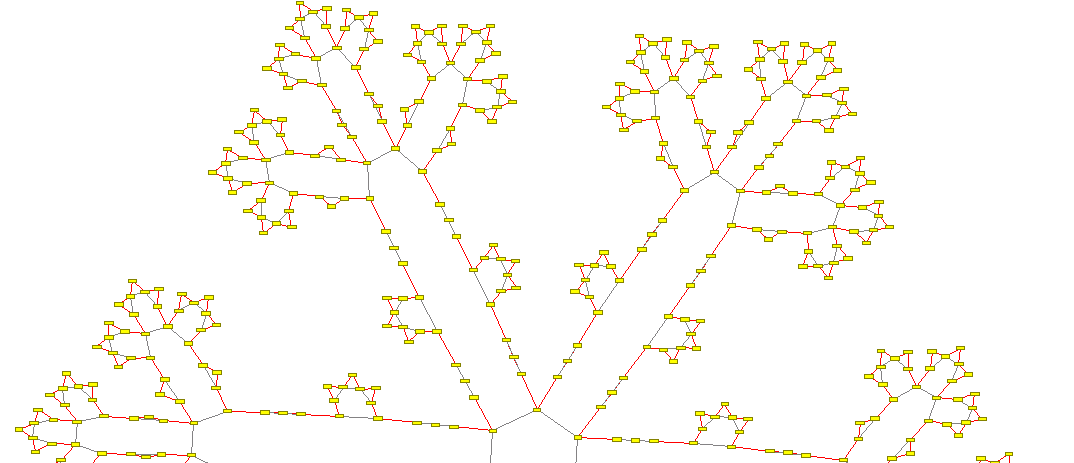
\includegraphics[width=0.9\linewidth]{fig/title}\\[6ex]
  \LARGE Jakob Blomer \qquad Rubino Gei\ss\\ \qquad Edgar Jakumeit\\[3ex]
  \large \today\\
  
%  \vfill
%	\large Technical Report 2007-5\\
%	\large ISSN 1432-7864	

  \setlength{\parindent}{\saveparindent}
\end{titlepage}
\clearpage

\chapter*{Abstract}

\parpic[l] {

\includegraphics[width=45mm]{fig/grgen-256.png}
}

\noindent \textsc{GrGen.NET} is a graph rewrite tool enabling elegant and convenient development of graph rewriting applications with comparable performance to conventionally developed ones.
\GrG\ uses attributed, typed, and directed multigraphs with multiple inheritance on node and edge types.
Extensive graphical debugging integrated into an interactive shell complements the feature highlights of \GrG.
This user manual contains both, normative statements in the sense of a reference manual as well as an informal guide to the features and usage of \GrG.\\[6ex]

\noindent This is a draft; it is published early because it is useful as-is, due to the many changes since the last version of the manual. 
Note: Especially the index and the internal references are broken.


\chapter*{Old Foreword}
First of all a word about the term ``graph rewriting''.
Some would rather say ``graph transformation''; some even think there is a difference between these two.
We don't see such differences and use graph rewriting for consistency.

The \textsc{GrGen} project started in spring 2003 with the diploma thesis of Sebastian Hack under supervision of Rubino Gei\ss.
At that time we needed a tool to find patterns in graph based intermediate representations used in compiler construction.
We imagined a tool that is fast, expressive, and easy to integrate into our compiler infrastructure.
So far Optimix\cite{assmann00graph} was the only tool that brought together the areas of compiler construction and graph rewriting.
However its approach is to feature many provable properties of the system per se, such as termination, confluence of derivations, and complete coverage of graphs.
This is achieved by restricting the expressiveness of the whole formalism below Turing-completeness.
Our tool \textsc{GrGen} in contrast should be Turing-complete.
Thus \GrG\ provides the user with strong expressiveness but leaves the task of proving such properties to the user.

To get a prototype quickly, we delegated the costly task of subgraph matching to a relational database system~\cite{Hac:03}.
Albeit the performance of this implementation could be improved substantially over the years, we believed that there was more to come.
Inspired by the PhD thesis of Heiko D\"orr~\cite{doerr} we reimplemented our tool to use search plan driven graph pattern matching of its own.
This matching algorithm evolved over time~\cite{adam,Bat:05:SA,Bat:05:DA,Bat:06,BKG:07} and has been ported from C to C\#~\cite{KG:07,Kro:07}. 
In the year 2005 Varr\'o~\cite{gramot2005_adapt} independently proposed a similar search plan based approach.

Though we started four years ago to facilitate some compiler construction problems, in the meantime \GrG\ has grown into a general purpose tool for graph rewriting.\\[3ex]

We want to thank all co-workers and students that helped during the design and implementation of \GrG\ as well as the writing of this manual.
Especially we want to thank Dr.~Sebastian Hack, G.~Veit Batz, Michael Beck, Tom Gelhausen, Moritz Kroll, Dr.~Andreas Ludwig, and Dr.~Markus Noga.
Finally, all this would not happened without the productive atmosphere and the generous support that Prof.~Goos provides at his chair.\\[3ex]

We wish all readers of the manual---and especially all users of \GrG---a pleasant graph rewrite experience.
We hope you enjoy using \GrG\ as much as we enjoy developing it.\\[3ex]

Thank you for using \GrG.\\[6ex]

\noindent Karlsruhe in July 2007, Rubino Gei\ss~on behalf of the \GrG-Team

%\pagebreak seems to be exactly one page

\chapter*{New Foreword}

Since the last version of this manual which was written for \GrG\ v1.4 a lot has happened, 
as can be seen quite easily in the fact that this manual describes \GrG\ v2.6.
The porting of C to C\# \cite{Kro:07} allowed for a faster pace of development,
which yielded alternatives and subpatterns allowing for structural recursion \cite{Jak:08,StructuralRecursion},
undirected edge support plus fine grain pattern condition \cite{SABuchwald:2008}, 
a data model more user friendly at the API, support for visited flags, 
and an prototypical implementation of an embedding of \GrG\ as s domain specific language into C\# \cite{DAMoritz}
-- resulting in \GrG\ v2.0.
\\[1ex]

Then Dr. Rubino Gei\ss~finished his dissertation \cite{DissRuby} and left, and Prof. Goos retired.
The succeeding Professor had no interested in graph rewriting,
so \GrG\ switched from a university project developed by students in their bachelor/masters thesis's
to an open source project (which is still hosted at the IPD, reachable from \url{www.grgen.net}).

And development continued:
With the introduction of generic set and map types in the model language to facilitate uses in computer linguistics
and in the rule control language to allow for more concise rule combinations.
With the 2+n pushdown automaton for matching patterns with structural recursion extended 
to handle pattern cardinality specifications and positive applications conditions.
With massive API improvements, now featuring an interface of typed, named entities in addition to the old name string and object based interface.
With the introduction of importers and exporters for GXL (the quasi standard graph exchange format in graph rewriting),
and for GRS, a much easier and less bloated native format.

Most of these features were introduced due to feedback from users and use cases:\\
We want to thank the organizers of GraBaTs\cite{grabats}, the annual meeting of the graph rewrite tool community,
which gave us the possibility to ruthlessly steal the best ideas of the competing tools.
Thanks to Berthold Hoffmann, for his ``french''-courses and the ideas about how to handle program graphs.
And thanks to several early users giving valuable feedback or even code (which is of course the best contribution you can give to an open source project), by name: 
Tom Gelhausen and Bugra Derre (you may have a look at \url{https://svn.ipd.uni-karlsruhe.de/trac/mx/wiki/Home} for some interesting results of this work at IPD Tichy), Paul Bedaride, Normen Müller, and Nicholas Tung.
\\[1ex]

\noindent Regarding questions please contact the \GrG-Team \foototesize{(currently consisting of Sebastian Buchwald, Rubino Gei\ss, Edgar Jakumeit, Moritz Kroll)}
via email to \texttt{grgen} at the host given by \texttt{ipd.info.uni-karlsruhe.de}.\\[2ex]

\noindent We hope you enjoy using \GrG\ even more than we enjoyed developing it\\ (it was fun but had its lengths from time to time ;).
\\[2ex]

Thank you for using \GrG.\\[3ex]

\noindent Karlsruhe in December 2009, Edgar Jakumeit on behalf of the \GrG-Team


\clearpage

\tableofcontents

\chapter{Introduction}
\pagenumbering{arabic}


\section{What is \GrG?}

{\scshape GrGen} (\textsc{G}raph \textsc{R}ewrite \textsc{Gen}erator) is a generative programming system for graph rewriting.
For the potentially expensive matching problem, {\scshape GrGen} applies several novel heuristic optimizations.
According to \indexed{Varr\'o's benchmark}, it is at least one order of magnitude faster than any other tool known to us.

In order to accelerate the matching step, we internally introduce \newterm{search plans} to represent different \newterm{matching strategies} and equip these search plans with a cost model, taking the present host graph into account.
The task of selecting a good search plan is then considered as an optimization problem~\cite{BKG:07,Bat:06}.
For the rewrite step, our tool implements the well-founded \newterm{single-pushout approach} (SPO, for explanation see~\cite{spoapproach}).

For ease of use, {\scshape GrGen} features an expressive specification language and generates program code with a convenient interface.
In contrast to systems like \indexed{Fujaba}~\cite{fujaba} our pattern matching algorithm is fully automatic and does not need to be tuned or partly be implemented by hand.
\GrG~\cite{grgen_web} is the successor of the \textsc{GrGen} tool presented at ICGT 2006~\cite{GBGHS:06}. 
The ``.NET'' postfix of the new name indicates that \textsc{GrGen} has been reimplemented in C\# for the Microsoft .NET or Mono environment~\cite{NET,MONO}.


\section{Features of \GrG}

The process of graph rewriting can be divided into four steps:
Representing a graph according to a model, searching a pattern aka finding a match, performing changes to the matched spot in the host graph, and, finally, selecting the next rule(s) for application.
We have organized the features of \GrG\ according to this breakdown of graph rewriting.

\begin{itemize}
  \item The graph model (meta-model) supports:
  \begin{itemize}
    \item Directed graphs
    \item Typed nodes and edges, with multiple inheritance on types
    \item Node and edge types can be equipped with typed attributes (like structs)
    \item Multigraphs (including multiple edges of the same type)
    \item Connection assertions to restrict the ``shape'' of graphs
  \end{itemize}
  
  \item The pattern language supports:
  \begin{itemize}
    \item Plain isomorphic subgraph matching (injective mapping)
    \item Homomorphic matching for a selectable set of nodes/edges, so that the matching is not injective
    \item Attribute conditions (including arithmetic operations on the attributes)
    \item Type conditions (including powerful instanceof-like type expressions)
    \item Parameter passing to rules
    \item \indexed{Dynamic patterns} with iterative or recursive paths and graphs (yet to be implemented)
  \end{itemize}
  
  \item The rewrite language supports:
  \begin{itemize}
    \item Attribute re-calculation (using arithmetic operations on the attributes)
    \item Retyping of nodes/edges (a stronger version of casts known from common programming languages)
    \item Creation of new nodes/edges of statically as well as dynamically computed types (some kind of generic templates)
    \item Two modes of specification: A rule can either express changes to be made to the match or replace the whole match (the semantics is always mapped to SPO)
    \item Returning certain edges/nodes for further computations
	  \item Copying (duplicating) of elements form the match---comparable with \indexed{sesqui-pushout} rewriting~\cite{CHHK:06} (yet to be implemented)
  \end{itemize}
  
  \item The rule application language (\GrShell) supports:
  \begin{itemize}
    \item Composing several rules with logical and iterative sequence control (called graph rewrite sequences, GRS)
    \item Various methods for creation/deletion/input/output of graphs/nodes/edges 
    \item Stepwise and graphic debugging of rule application
    \item Graph rewrite sequences that can contain nested transactions\indexmain{transaction, nested}
  \end{itemize}
  
  \item Alternatively to \GrShell, you can access the match and rewrite facility through \LibGr. In this way you can build your own algorithmic rule applications in a .NET language of your choice. 
\end{itemize}


\section{System Overview}

Figure~\ref{figsys} gives an overview of the \GrG\ system components. Table~\ref{dirstruc} shows the \GrG\ directory structure.

\begin{figure}[htbp]
  \centering
	\scalebox{0.8}{
  \begin{tikzpicture}
      \begin{scope}[shape=rectangle,minimum size=0.75cm,text width=3cm,text centered]
          \tikzstyle{every node}=[draw]
          \node (spec1)    at (0   ,0)    {Rewrite Rules\indexmain{rewrite rule} (*\indexed{.grg})};
          \node (spec2)    at (0   ,2)    {Graph Model\indexmain{graph model} (*\indexed{.gm})};
          \node (grgen)    at (4   ,1)    {\GrG\ Generator\indexmain{generator} (Java, C\#)};
          \node (rewriter) at (10  ,0)    {Rewrite~Rules (C\#)};
          \node (types)    at (10  ,2)    {Graph~Model (C\#)};
          \node (data)     at (14  ,1)    {Graph~Management (C\#)};
          \node (libgr)    at (12  ,4)    {\LibGr\indexmain{libGr}\ (C\#)};
          \node[fill,color=gray] (app)      at (14.1  ,5.6)  {};
          \node[fill=white] (app)      at (14  ,5.5)  {Applications};
          \node (grsh)     at (10  ,5.5)  {\GrShell\indexmain{GrShell}\ (C\#)};
          \node (grs)      at (6   ,5.5)  {Graph Rewrite Script\indexmain{graph rewrite script}\indexmainsee{GrShell script}{graph rewrite script}\indexmainsee{script}{graph rewrite script} (*\indexed{.grs})};
      \end{scope}

      \node[draw, minimum width=9cm,minimum height=4cm] (engine) at (12,1) {};
      \node[draw, minimum width=9cm,minimum height=4cm,style=dotted] (ct) at (2,1) {};
      \node[anchor=north east] (engine_lab) at (engine.north east) {Backend\indexmain{backend} (Run Time)};
      \node[anchor=north east] (ct_lab) at (ct.north east) {Frontend (Compile Time)};

      \draw[->,dashed,red,>=triangle 45]     (spec1)   -> (grgen);
      \draw[->,dashed,red,>=triangle 45]     (spec2)   -> (grgen);
      \draw[->,dashed,red,>=triangle 45]     (grgen)   -> (types);
      \draw[->,line width=1pt,>=triangle 45] (grgen)   -> (engine);
      \draw[->,dashed,red,>=triangle 45]     (grgen)   -> (rewriter);
      \draw[->,line width=1pt,>=triangle 45] (app)     -> (libgr);
      \draw[->,line width=1pt,>=triangle 45] (grsh)    -> (libgr);
      \draw[->,dashed,red,>=triangle 45]     (grs)     -> (grsh);
      \draw[->,line width=1pt,>=triangle 45] (libgr)   -> (engine);

      \draw[->,line width=1pt,>=triangle 45] (-1.75,5.5) -- +(2.5,0) node[above, midway] {call};
      \draw[->,dashed,red,>=triangle 45] (-1.75,4.5)  -- +(2.5,0) node[above, midway] {read / generate};
  \end{tikzpicture}
	}
  \caption{\GrG\ system components~\cite{Kro:07}}
  \label{figsys}
\end{figure}
\begin{table}[htbp]
  \begin{tabularx}{\linewidth}{|lX|} \hline
  bin & Contains the .NET assemblies, in particular \indexed{GrGen.exe} (the graph rewrite system generator), \indexed{lgspBackend.dll} (a \GrG\ backend), \indexed{LibGr.dll} (the backend API), and the shell \indexed{GrShell.exe}.  \\ 
  lib & Contains the \GrG\ generated assemblies (*.dll). \\
  specs & Contains the graph rewrite system source documents (*.gm and *.grg). \\ \hline
  \end{tabularx}
  \caption{\GrG\ directory structure}
  \label{dirstruc}
\end{table}

A graph rewrite system\footnote{In this context, system is not a CH0-like grammar rewrite system, but rather a set of interacting software components.} is defined by a rule set file (*.grg) and zero or more graph model description files (*.gm). 
Such a graph rewrite system is generated from these specifications by GrGen.exe and can be used by applications such as \GrShell.
Figure~\ref{process} shows the generation process.

\begin{figure}[htbp]
  \centering
	\scalebox{0.8}{
  \begin{tikzpicture}
      \begin{scope}[shape=rectangle,minimum size=0.75cm,text width=3cm,text centered]
          \tikzstyle{every node}=[draw]
          \node (gm1)      at (0   ,0)    {model1.gm};
          \node (gm2)      at (0   ,1)    {model2.gm};
          \node (gm3)      at (0   ,2)    {model3.gm};
          \node (grg)      at (4.5 ,1)    {rules1.grg};
          \node (grgen)    at (10   ,1)    {GrGen.exe};
          \node (act)      at (15.5,1) {rules1Actions.dll};
          \node (backend)  at (10   ,2)    {backend.dll};
          \node (mod)      at (15.5,2)  {rules1Model.dll};
      \end{scope}
         
			\draw[|-|] (-1,-1.5)   -- (5.5, -1.5)    node[below, midway] {/specs};
			\draw[|-|] (9,-1.5)    -- (11, -1.5)     node[below, midway] {/bin};
			\draw[|-|] (14.5,-1.5) -- (16.5, -1.5)   node[below, midway] {/lib};

      \draw[->,line width=1pt,>=triangle 45]     (grg)     -> (gm1);
      \draw[->,line width=1pt,>=triangle 45]     (grg)     -> (gm2);
      \draw[->,line width=1pt,>=triangle 45]     (grg)     -> (gm3);
      \draw[->,dashed,red,>=triangle 45]         (grg)     -> (grgen);
      \draw[->,dashed,red,>=triangle 45]         (grgen)   -> (mod);
      \draw[->,dashed,red,>=triangle 45]         (grgen)   -> (act);
      \draw[->,line width=1pt,>=triangle 45]     (mod)     -> (backend);
      \draw[->,line width=1pt,>=triangle 45]     (act)     -> (backend);


      \draw[->,line width=1pt,>=triangle 45] (-1.25,3.5) -- +(2.5,0) node[above, midway] {referencing};
      \draw[->,dashed,red,>=triangle 45]     (3.25,3.5)  -- +(2.5,0) node[above, midway] {read / generate};
  \end{tikzpicture}
	}
  \caption{Generating a graph rewrite system}
  \label{process}
\end{figure}

In general you have to distinguish carefully between a graph model (meta level), a host graph, a pattern graph and a rewrite rule.
In \GrG\ pattern graphs are implicitly defined by rules, i.e.\ each rule defines its pattern.
On the technical side, specification documents for a graph rewrite system can be available as source documents for graph models and rule sets (plain text *.gm and *.grg files) or as their translated .NET modules, either C\# source files or their compiled assemblies (*.dll).

Generating a \GrG\ graph rewrite system may be considered as preliminary task.
The actual process of rewriting as well as dealing with host graphs is performed by \GrG's backend.
\GrG\ provides a backend \indexed{API}---the .NET library \LibGr.
For most issues---in particular for experimental purposes---you might rather want to work with the \GrShell\ because of its more convenient interface.
However, \GrShell\ does not provide the full power of the \LibGr; see also note~\ref{note:indeterminism} on page~\pageref{note:indeterminism}.

\section{What is Graph Rewriting?}
\label{ov:whatsallabout}

The notion of graph rewriting as understood by \GrG\ is a method for declaratively specifying ``changes'' to a graph.
This is comparable to the well-known term rewriting. 
Normally you use one or more \newterm{graph rewrite rules} to accomplish a certain task.
\GrG\ implements an SPO-based approach.
In the simplest case such a graph rewrite rule consists of a tuple $L \rightarrow R$, whereas $L$---the \newterm{left hand side}\indexmainsee{LHS}{left hand side} of the rule---is called \newterm{pattern graph} and $R$---the \newterm{right hand side}\indexmainsee{RHS}{right hand side} of the rule---is the \newterm{replacement graph}.

\begin{figure}[htbp]
	\centering
  \begin{tikzpicture}
    \begin{scope}[minimum size=0.5cm]
      \tikzstyle{every node}=[draw]
      \node (L)     at (0   ,2.5) {$L$};
      \node (R)     at (7   ,2.5) {$R$};
      \node (mL)    at (0   ,0) {};
      \node (mR)    at (7   ,0) {};
      \node[text width=2cm,text badly ragged,minimum size=1cm] (H)     at (0   ,0) {$H$};
      \node[text width=2cm,text badly ragged,minimum size=1cm] (Hs)    at (7   ,0) {$H'$};
    \end{scope}

    \draw[dotted,->] (L) node[above=0.4cm] {Pattern Graph} -> (mL) node[left,midway]  {Match $m$}   node[below=0.6cm] {Host Graph};
    \draw[dotted,->] (R) node[above=0.4cm] {Rewrite Graph} -> (mR)                              node[below=0.6cm] {Result Graph};

    \pgfsetshortenstart{0.5cm}
    \pgfsetshortenend{0.5cm}
    \draw[thick,->]  (L) -> (R)  node[above,midway] {Preservation Morphism $r$} node[below,midway] {Rule};
    \draw[thick,->]  (H) -> (Hs) node[below,midway] {Rule Application};
  \end{tikzpicture}
  \caption{Basic Idea of Graph Rewriting}
  \label{figrule}
\end{figure}

Moreover we need to identify graph elements (nodes or edges) of $L$ and $R$ for preserving them during rewrite. 
This is done by a \newterm{preservation morphism} $r$ mapping elements from $L$ to $R$; the morphism $r$ is injective, but needs to be neither surjective nor total.
Together with a rule name $p$ we have $p : L \xrightarrow{r} R$.

The transformation is done by \newterm{application}\indexmainsee{rule application}{application} of a rule to a \newterm{host graph} $H$.
To do so, we have to find an occurrence of the pattern graph in the host graph. 
Mathematically speaking, such a \newterm{match} $m$ is an isomorphism from $L$ to a subgraph of $H$.
This morphism may not be unique, i.e.\ there may be several matches.
Afterwards we change the matched \indexed{spot} $m(L)$ of the host graph, such that it becomes an isomorphic subgraph of the replacement graph $R$.
Elements of $L$ not mapped by $r$ are deleted from $m(L)$ during rewrite.
Elements of $R$ not in the image of $r$ are inserted into $H$, all others (elements that are mapped by $r$) are retained.
The outcome of these steps is the resulting graph $H'$. In symbolic language: $H \xRightarrow{m, p} H'$.


\section{An Example}
\label{ov:example}

We'll have a look at a small example. 
Graph elements (nodes and edges) are labeled with and identifier.
If a type is necessary then it is stated after a colon.
We start using a special case to construct our host graph: an \indexed{empty pattern} always produces exactly one\footnote{Because of the uniqueness of the total and totally undefined morphism.} match (independent of the host graph). So we construct an apple by applying
\[
  p_0:  
  \begin{array}[c]{c} 
    \emptyset
  \end{array} 
  \begin{array}[c]{c} 
    \longrightarrow 
  \end{array} 
  \begin{array}[c]{c} 
    \begin{tikzpicture}[show background rectangle]
      \tikzstyle{every node}=[circle]
      \node[draw] (n1) at (2.5,5) {};
      \node[draw] (n2) at (2,4)   {};
      \node[draw] (n3) at (0,2)   {};
      \node[draw] (n4) at (2,0)   {};
      \node[draw] (n5) at (4,2)   {};
    	
    	\draw[-latex] (n2) --                                  (n1) node[left,midway]  {$e_1$};
    	\draw[-latex] (n2) .. controls +(-1,1) and +(0,1) ..   (n3) node[left,midway]  {$e_2$};
      \draw[-latex] (n3) .. controls +(0,-1) and +(-1,0) ..  (n4) node[left,midway]  {$e_3$};
    	\draw[-latex] (n4) .. controls +(1,0)  and +(0,-1) ..  (n5) node[right,midway] {$e_4$};
      \draw[-latex] (n5) .. controls +(0,1)  and +(1,1) ..   (n2) node[right,midway] {$e_5$};
    \end{tikzpicture}
  \end{array}
\]
to the empty host graph. 
As the result we get an apple as new host graph $H$. 
Now we want to rewrite our apple with stem to an apple with a leaflet. 
So we apply
\[
  p_1:
  \begin{array}[c]{c}
    \begin{tikzpicture}[show background rectangle]
      \tikzstyle{every node}=[circle,minimum size=0.7cm]
      \node[draw] (a) at (2,5.5)  {a};
      \node[draw] (b) at (2,4)    {b};
    	
    	\draw[-latex] (b) -- (a) node[left,midway]  {$x$};
    \end{tikzpicture}
  \end{array}
  \begin{array}[c]{c}
    \longrightarrow
  \end{array}
  \begin{array}[c]{c}
    \begin{tikzpicture}[show background rectangle]
      \tikzstyle{every node}=[circle,minimum size=0.7cm]
      \node[draw] (c) at (2,5.5)  {c};
      \node[draw] (b) at (2,4)    {b};
    	
    	\draw[-latex] (b) .. controls +(-0.7,+0.7) and +(-0.7,-0.7) .. (c) node[left,midway]   {$y$};
    	\draw[-latex] (b) .. controls +(+0.7,+0.7) and +(+0.7,-0.7) .. (c) node[right,midway]  {$z$};
    \end{tikzpicture}
  \end{array} 
\]
to $H$ and get the new host graph $H_1$, something like this:
\[
  \begin{array}[c]{c} 
    \begin{tikzpicture}[show background rectangle]
      \tikzstyle{every node}=[circle]
      \node[draw] (n1) at (2.5,5) {};
      \node[draw] (n2) at (2,4)   {};
      \node[draw] (n3) at (0,2)   {};
      \node[draw] (n4) at (2,0)   {};
      \node[draw] (n5) at (4,2)   {};
    	
    	\draw[-latex] (n2) --                                  (n1) node[left,midway]  {$e_1$};
    	\draw[-latex] (n2) .. controls +(-1,1) and +(0,1) ..   (n3) node[left,midway]  {$e_2$};
      \draw[-latex] (n3) .. controls +(0,-1) and +(-1,0) ..  (n4) node[left,midway]  {$e_3$};
    	\draw[-latex] (n4) .. controls +(1,0)  and +(0,-1) ..  (n5) node[right,midway] {$e_4$};
      \draw[-latex] (n5) .. controls +(0,1)  and +(1,1) ..   (n2) node[right,midway] {$e_5$};
    \end{tikzpicture}
  \end{array} 
  \begin{array}[c]{c} 
    \xRightarrow{\quad p_1 \quad}
  \end{array} 
  \begin{array}[c]{c} 
    \begin{tikzpicture}[show background rectangle]
      \tikzstyle{every node}=[circle]
      \node[draw] (n1) at (2.5,5) {};
      \node[draw] (n2) at (2,4)   {};
      \node[draw] (n3) at (0,2)   {};
      \node[draw] (n4) at (2,0)   {};
      \node[draw] (n5) at (4,2)   {};
      \node[draw] (n6) at (0,0.5)   {};
    	
    	\draw[-latex] (n2) --                                  (n1) node[left,midway]  {$e_1$};
    	\draw[-latex] (n2) .. controls +(-1,1) and +(0,1) ..   (n3) node[left,midway]  {$e_2$};
      \draw[-latex] (n3) .. controls +(-0.7,-0.7) and +(-0.7,+0.7) .. (n6) node[left,midway]  {$e_6$};
      \draw[-latex] (n3) .. controls +(+0.7,-0.7) and +(+0.7,+0.7) .. (n6) node[right,midway] {$e_7$};
    	\draw[-latex] (n4) .. controls +(1,0)  and +(0,-1) ..  (n5) node[right,midway] {$e_4$};
      \draw[-latex] (n5) .. controls +(0,1)  and +(1,1) ..   (n2) node[right,midway] {$e_5$};
    \end{tikzpicture}
  \end{array}
\]
What happened? 
\GrG\ has arbitrarily chosen one match out of the set of possible matches, because $x$ matches edge $e_3$ as well as $e_1$.
A correct solution could make use of edge type information. 
We have to change rule $p_0$ to generate the edge $e_1$ with a special type ``stem''.
And this time we will even keep the stem. 
So let
\[
  p_2:
  \begin{array}[c]{c}
    \begin{tikzpicture}[show background rectangle]
      \tikzstyle{every node}=[circle,minimum size=0.7cm]
      \node[draw] (a) at (2,5.5)  {a};
      \node[draw] (b) at (2,4)    {b};
    	
    	\draw[-latex] (b) -- (a) node[left,midway]  {$x:\text{stem}$};
    \end{tikzpicture}
  \end{array}
  \begin{array}[c]{c}
    \longrightarrow
  \end{array}
  \begin{array}[c]{c}
    \begin{tikzpicture}[show background rectangle]
      \tikzstyle{every node}=[circle,minimum size=0.7cm]
      \node[draw] (c) at (2,5.5)  {c};
      \node[draw] (b) at (2,4)    {b};
      \node[draw] (a) at (3.5,5.5){a};
    	
    	\draw[-latex] (b) -- (a) node[right,midway]  {$x$};
    	\draw[-latex] (b) .. controls +(-0.7,+0.7) and +(-0.7,-0.7) .. (c) node[left,midway]   {$y$};
    	\draw[-latex] (b) .. controls +(+0.7,+0.7) and +(+0.7,-0.7) .. (c) node[above,midway]  {$z$};
    \end{tikzpicture}
  \end{array}.
\]
If we apply $p_2$ to the modified $H_1$ this leads to
\[
  \begin{array}[c]{c} 
    \begin{tikzpicture}[show background rectangle]
      \tikzstyle{every node}=[circle]
      \node[draw] (n1) at (2.5,5) {};
      \node[draw] (n2) at (2,4)   {};
      \node[draw] (n3) at (0,2)   {};
      \node[draw] (n4) at (2,0)   {};
      \node[draw] (n5) at (4,2)   {};
    	
    	\draw[-latex] (n2) --                                  (n1) node[left,pos=0.8]  {$e_1:\text{stem}$};
    	\draw[-latex] (n2) .. controls +(-1,1) and +(0,1) ..   (n3) node[left,midway]  {$e_2$};
      \draw[-latex] (n3) .. controls +(0,-1) and +(-1,0) ..  (n4) node[left,midway]  {$e_3$};
    	\draw[-latex] (n4) .. controls +(1,0)  and +(0,-1) ..  (n5) node[right,midway] {$e_4$};
      \draw[-latex] (n5) .. controls +(0,1)  and +(1,1) ..   (n2) node[right,midway] {$e_5$};
    \end{tikzpicture}
  \end{array} 
  \begin{array}[c]{c} 
    \xRightarrow{\quad p_2 \quad}
  \end{array} 
  \begin{array}[c]{c} 
    \begin{tikzpicture}[show background rectangle]
      \tikzstyle{every node}=[circle]
      \node[draw] (n1) at (3,5) {};
      \node[draw] (n2) at (2,4)   {};
      \node[draw] (n3) at (0,2)   {};
      \node[draw] (n4) at (2,0)   {};
      \node[draw] (n5) at (4,2)   {};
      \node[draw] (n6) at (2,5.0)   {};
    	
    	\draw[-latex] (n2) --                                  (n1) node[right,pos=0.6] {$e_1:\text{stem}$};
    	\draw[-latex] (n2) .. controls +(-1,1) and +(0,1) ..   (n3) node[left,midway]  {$e_2$};
      \draw[-latex] (n3) .. controls +(0,-1) and +(-1,0) ..  (n4) node[left,midway]  {$e_3$};
    	\draw[-latex] (n4) .. controls +(1,0)  and +(0,-1) ..  (n5) node[right,midway] {$e_4$};
      \draw[-latex] (n5) .. controls +(0,1)  and +(1,1) ..   (n2) node[right,midway] {$e_5$};
    	\draw[-latex] (n2) .. controls +(-0.3,+0.3) and +(-0.3,-0.3) .. (n6) node[left,midway]   {};
    	\draw[-latex] (n2) .. controls +(+0.3,+0.3) and +(+0.3,-0.3) .. (n6) node[right,midway]  {};
    \end{tikzpicture}
  \end{array}.
\]

\section{The Tools}

All the programs and libraries of \GrG\ are licensed under \indexed{LGPL}. Notice that the \yComp\ graph viewer is not a part of \GrG ; \yComp\ ships with its own license. Although \yComp\ is not free software, it's free for use in academic and non-commercial areas.

\subsection{\texttt{\indexed{GrGen.exe}}}
The \texttt{GrGen.exe} assembly implements the \GrG\ generator. The \GrG\ generator parses a rule set and its model files and compiles them into .NET assemblies. The compiled assemblies interact with the \GrG\ backend.
\begin{description}
  \item[Usage] \texttt{[mono] GrGen.exe [-use <existing-dir>] [-keep] <rule-set> [<output-dir>]}\\
    \emph{rule-set} is a file containing a rule set specification according to chapter~\ref{chaprulelang}. Usually such a file has the suffix \texttt{\indexed{.grg}}. The suffix \texttt{.grg} may be omitted.
By default \GrG\ tries to write the compiled assemblies to the directory \texttt{../lib} relative to the path of \texttt{GrGen.exe}. This can be changed by the optional parameter \emph{output-dir}.
  \item[Options] \mbox{} 
    \begin{tabularx}{\linewidth}{lX}
      \texttt{-keep} & Keep the generated C\# source files. A subdirectory \texttt{tmpgrgen$n$}\footnote{$n$ is an increasing number.} within the current directory will be created. This directory contains:
\begin{itemize}
  \item \texttt{printOutput.txt}---a snapshot of \texttt{stdout} during program execution.
  \item \emph{Name}\texttt{Actions.cs}---the C\# source file of the \emph{rule-set}\texttt{Actions.dll} assembly.
  \item \emph{Name}\texttt{Model.cs}---the C\# source file(s) of the \emph{rule-set}\texttt{Modell.dll} assembly.
\end{itemize}\\
      \texttt{-use} & Don't re-generate C\# source files. Instead use the files in \emph{existing-dir} to build the assemblies.	
    \end{tabularx}
  \item[Requires] .NET 2.0 (or above) or Mono 1.2.2 (or above). Java Runtime Environment 1.5 (or above).
\end{description}

\subsection{\texttt{\indexed{GrShell.exe}}}
The \GrShell\indexmain{GrShell} is a shell application of the \LibGr. \GrShell\ is capable of creating, manipulating, and dumping graphs as well as performing graph rewriting with graphical debug support. For further information about the \GrShell\ language see chapter~\ref{chapgrshell}.

\begin{description}
  \item[Usage] \texttt{[mono] grShell.exe [-c "<commands>" | <grshell-script>]}\\
     Opens the interactive shell. The \GrShell\ will execute the commands in \emph{grshell-script}\indexmain{graph rewrite script} (usually a \texttt{*\indexed{.grs}} file) immediately.  
  \item[Options] \mbox{} 
    \begin{tabularx}{\linewidth}{lX}
      \texttt{-c} & Execute the quoted \GrShell\ commands immediately. Instead of a line break use a double semicolon \texttt{;;} to separate commands.
    \end{tabularx}
  \item[Requires] .NET 2.0 (or above) or Mono 1.2.2 (or above).
\end{description}

\subsection{\texttt{\indexed{LibGr.dll}}}
The \LibGr\indexmain{libGr} is a .NET assembly implementing \GrG's \indexed{API}. See the extracted HTML documentation for interface descriptions. 

\subsection{\texttt{\indexed{yComp.jar}}}
\label{tools:ycomp}
\yComp\indexmain{yComp} \cite{ycomp} is a graph visualization tool based on \yFiles\ \cite{yfiles}. 
It is well integrated in \GrG, but it's not a part of \GrG. \yComp\ implements several graph layout algorithms and has file format support for \indexed{VCG}, GML and YGF among others. 
\begin{description}
  \item[Usage] Usually \yComp\ will be loaded by the \GrShell. You might want to open \yComp\ manually by typing\\
   \texttt{java -jar yComp.jar [<graph-file>]}\\
  The \emph{graph-file} may be any graph file in a supported format. \yComp\ will open this file on startup.
  \item[Hints] Do not use the \indexedsee{compiler graph}{layout algorithm} \indexed{layout algorithm} (\yComp's default setting). 
  Instead \texttt{\indexedsee{Organic}{layout algorithm}} or \texttt{\indexedsee{Orthogonal}{layout algorithm}} might be good choices. 
  Use the rightmost blue play button to start layout process. This may take a while, depending on the graph size:
\begin{center}
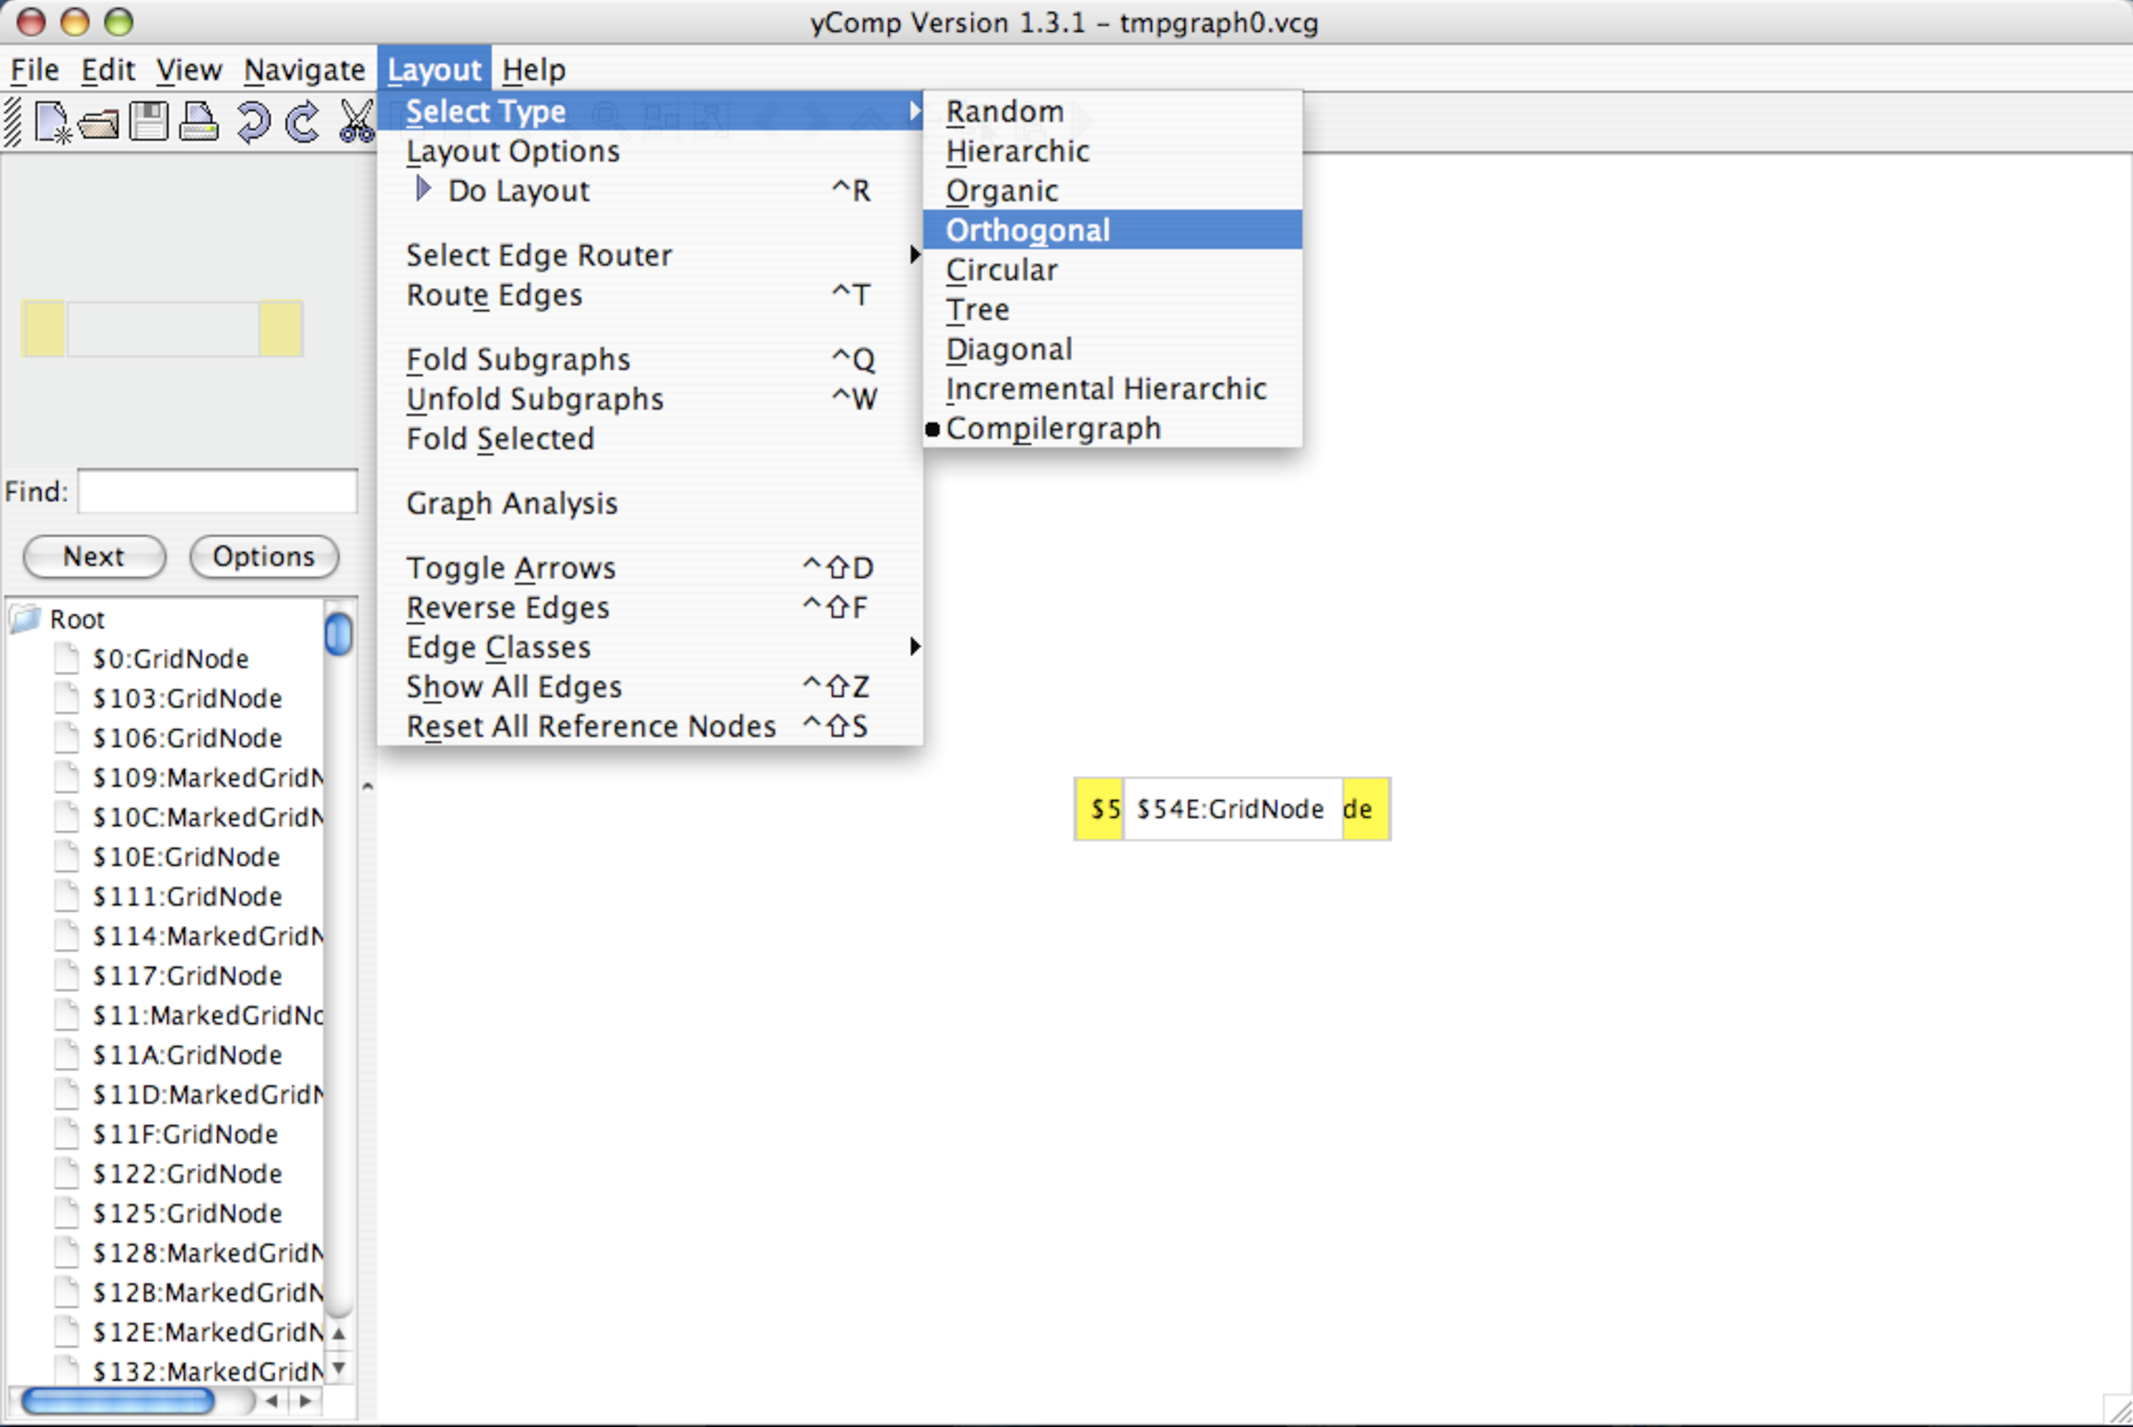
\includegraphics[width=0.45\linewidth]{fig/ycomp1.pdf} 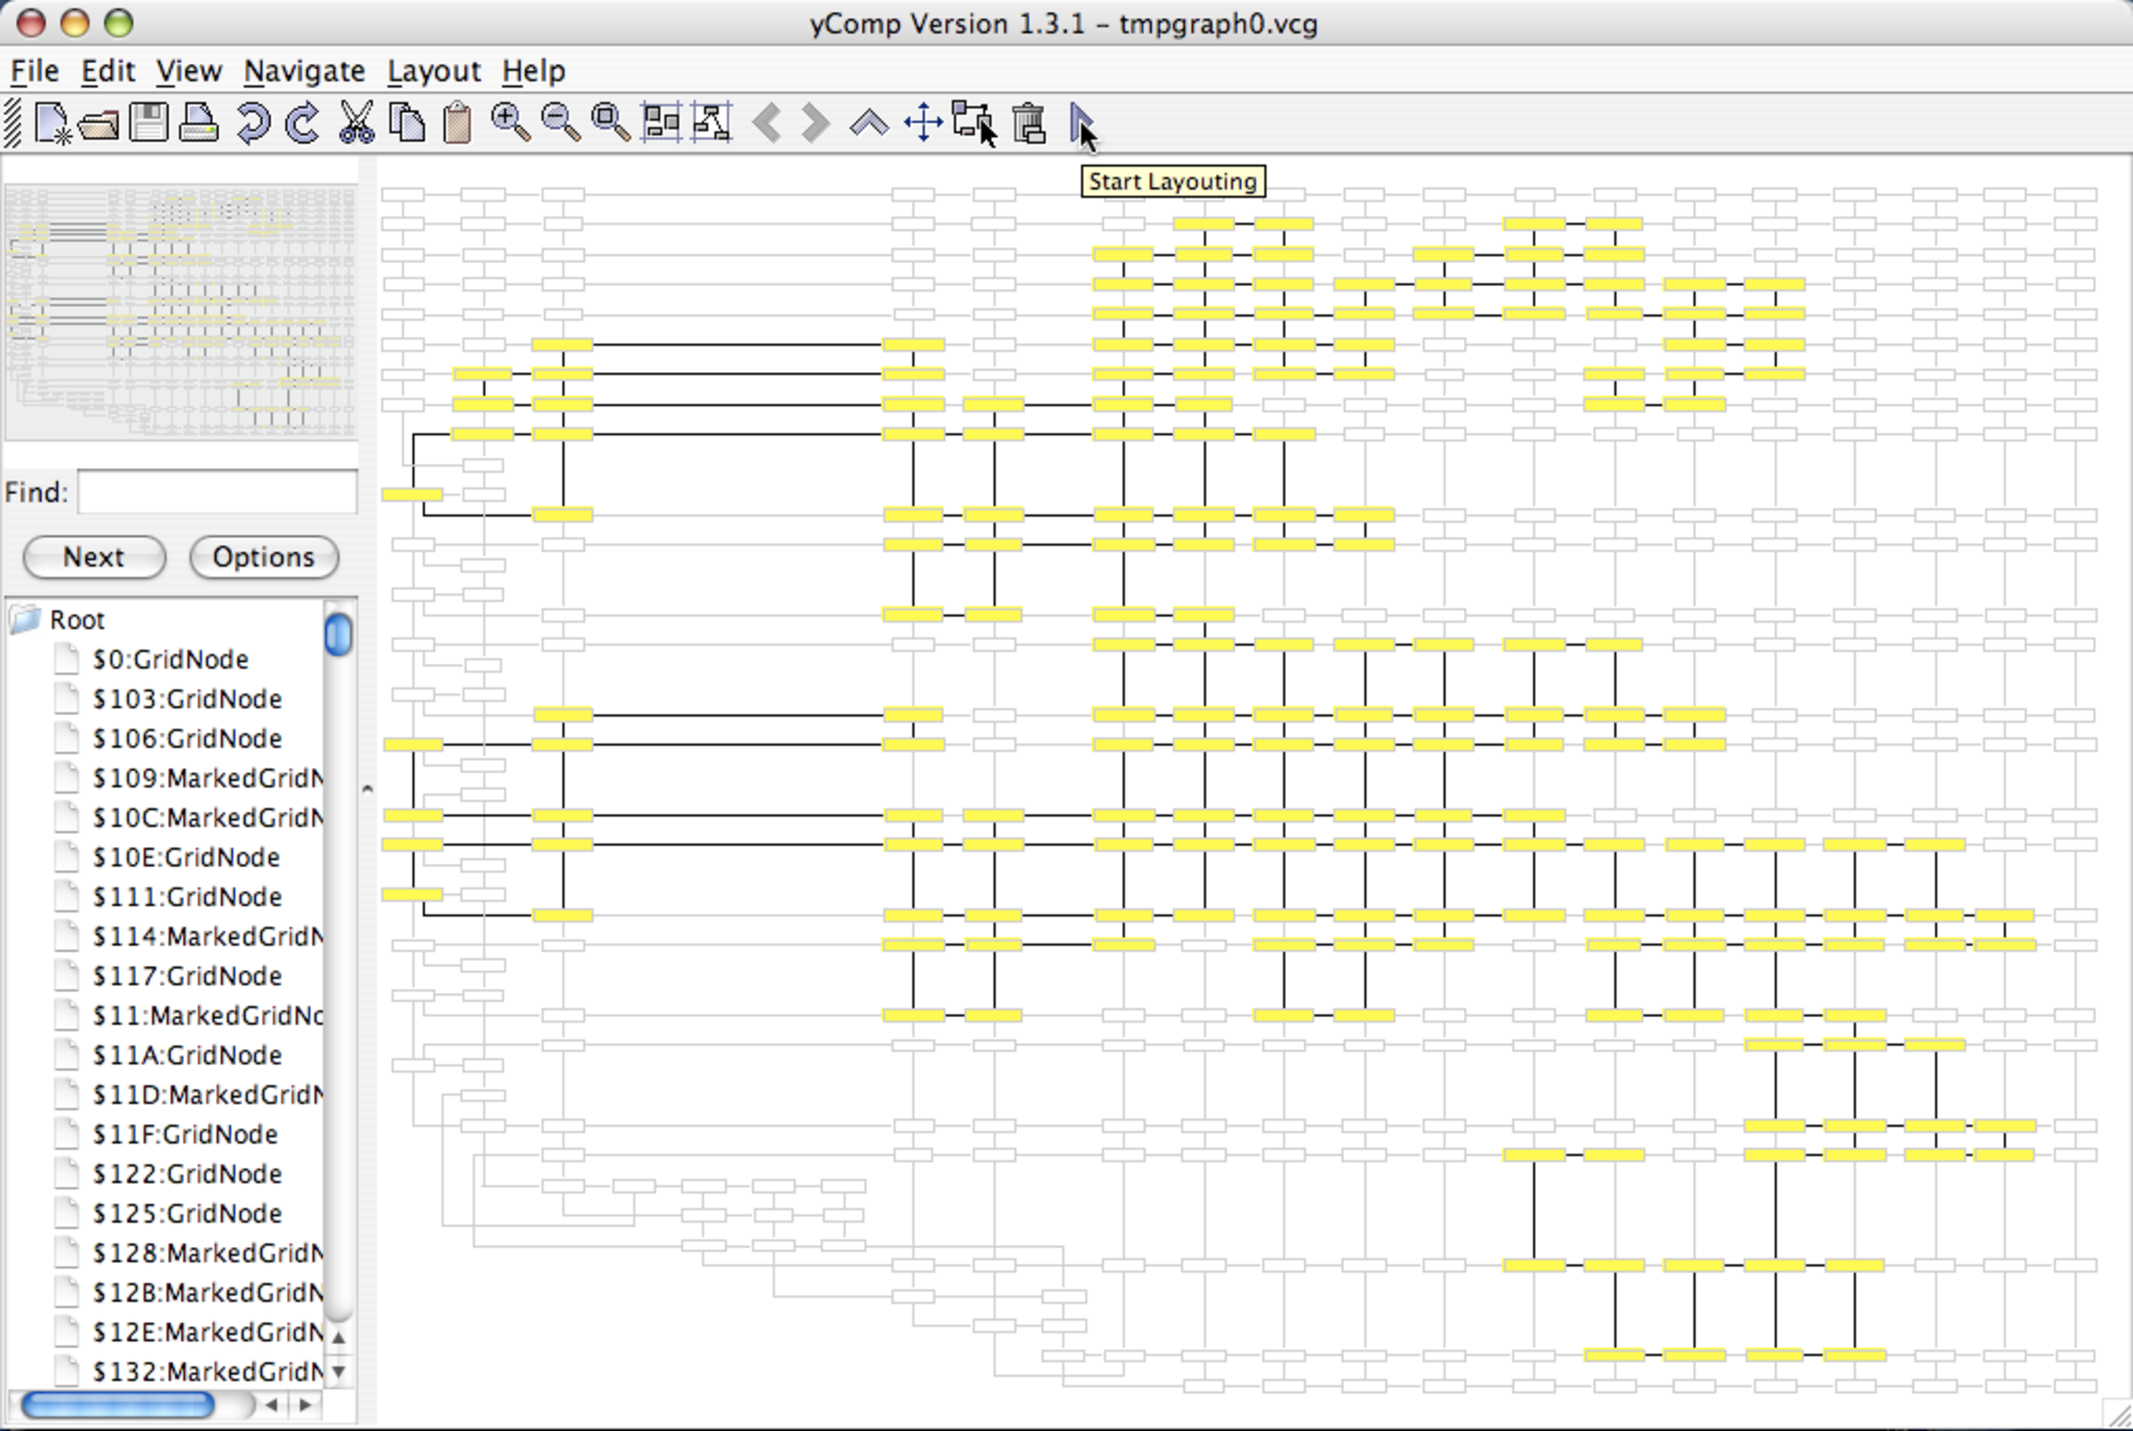
\includegraphics[width=0.45\linewidth]{fig/ycomp2.pdf}
\end{center}
  \item[Requires] Java Runtime Environment 1.5 (or above).
\end{description}




\chapter{Quickstart}\indexmain{quickstart}

In this chapter we'll build a \GrG\ system from scratch. 
You should already have read chapter \ref{chp:intro} to have a glimpse of the \GrG\ system and its components.
We will use \GrG\ to construct non-deterministic state machines.
We further show some actual graph rewriting by removing $\varepsilon$-transitions from our state machines.
This is not too much about details but rather about the \GrG\ look and feel.

\section{Downloading \& Installing}
If you are reading this document, you probably did already download the \GrG\ software from our website (\url{http://www.grgen.net}).
Make sure you have the following system requirements installed
\begin{itemize}
	\item Java 1.5 or above
	\item Mono 1.2.3 on Unix-like platforms / .NET 2.0 or above on Microsoft Windows 
\end{itemize}
Unpack the package to a directory of your choice, for example into \texttt{/opt/grgen} and \texttt{/opt/ycomp}:
\begin{bash}
mkdir /opt/grgen
tar xvfj GrGenNET-V1_3_1-2007-12-06.tar.bz2
mv GrGenNET-V1_3_1-2007-12-06/* /opt/grgen/
rmdir GrGenNET-V1_3_1-2007-12-06
\end{bash}
Add the \texttt{/opt/grgen/bin} directory to your search paths, for instance if you use \texttt{bash} add a line to your \texttt{/home/.profile} file.
\begin{bash}
export PATH=/opt/grgen/bin:$PATH
\end{bash}
Furthermore we create a directory for our \GrG\ data, for instance by \texttt{mkdir /home/grgen}.

\section{Creating a Graph Model}
In the directory \texttt{/home/grgen} we create a text file \texttt{state\_machine.gm} that contains the graph meta model for our state machine.
By graph meta model we mean a set of node types and edge types which are available for building state machine graphs (see chapter \ref{chapmodellang}).
Figure \ref{fig:quick:mm} shows the meta model.
\begin{figure}[htbp]
    \centering
    \begin{grgen}
node class State {
    id: int;
}

abstract node class SpecialState extends State;
node class StartState extends SpecialState;
node class FinalState extends SpecialState;
node class StartFinalState extends StartState, FinalState;

edge class Transition {
    Trigger: string;
}

const edge class EpsilonTransition extends Transition;    
    \end{grgen}
    \caption{Meta Model for State Machines}
    \label{fig:quick:mm}
\end{figure}    
What have we done?
You can see two base types, \texttt{State} for state nodes and \texttt{Transition} for transition edges that will connect the state nodes.
\texttt{State} has an integer attribute \texttt{id} and \texttt{Transition} has a string attribute \texttt{Trigger} which indicates the character sequence for switching from the source state node to the destination state node.
For the rest of the types we use inheritance (keyword \texttt{extends}) which works more or less like inheritance in object oriented languages.
Accordingly the \texttt{abstract} modifier for \texttt{SpecialState} means that you cannot create a node of that precise type, but you might create nodes of non-abstract subtypes.
As you can see \GrG\ supports multiple inheritance and with \texttt{StartFinalState} we have constructed a ``diamond'' type hierarchy.

\section{Creating Graphs}
\label{sct:quick:create}
Let's test our graph meta model by creating a state machine graph.
We will use the \GrShell\ (see chapter chapgrshell) and---for visualization---\yComp.
To get everything working we need a rule set file, too.
For the moment we just create an almost empty file \texttt{remove\_epsilons.grg} in the \texttt{/home/grgen} directory, containing only the line
\begin{grgen}
using state_machine;
\end{grgen}
Now, we could start by launching the \GrShell\ and typing the commands interactively.
This is, however, in most of the cases not the preferred way.
We rather create a \GrShell\ script, say \texttt{remove\_epsilons.grs}, in the \texttt{/home/grgen} directory.
Figure \ref{fig:quick:shell} shows this script.
Run the script by executing \texttt{grshell remove\_epsilons.grs}.
The first time you execute the script, it might take a while because \GrG\ has to compile the meta model and the rule set into .NET assemblies.
\begin{figure}[htbp]
    \centering
    \begin{grgen}
new graph remove_epsilons "StateMachineGraph"

new :StartState($=S, id=0)
new :FinalState($=F, id=3)
new :State($="1", id=1)
new :State($="2", id=2)
new @(S)-:Transition(Trigger="a")-> @("1")
new @("1")-:Transition(Trigger="b")-> @("2")
new @("2")-:Transition(Trigger="c")-> @(F)
new @(S)-:EpsilonTransition-> @("2")
new @("1")-:EpsilonTransition-> @(F)
new @(S)-:EpsilonTransition-> @(F)

show graph ycomp
    \end{grgen}
    \caption{Constructing a state machine graph in \GrShell}
    \label{fig:quick:shell}
\end{figure}
The graph viewer \yComp\ opens and you get a window similiar to figure \ref{fig:quick:ycomp} after clicking the blue ``layout graph'' button on the very right side of the button bar (see also section \ref{tools:ycomp}).
\begin{figure}[htbp]
	\centering
	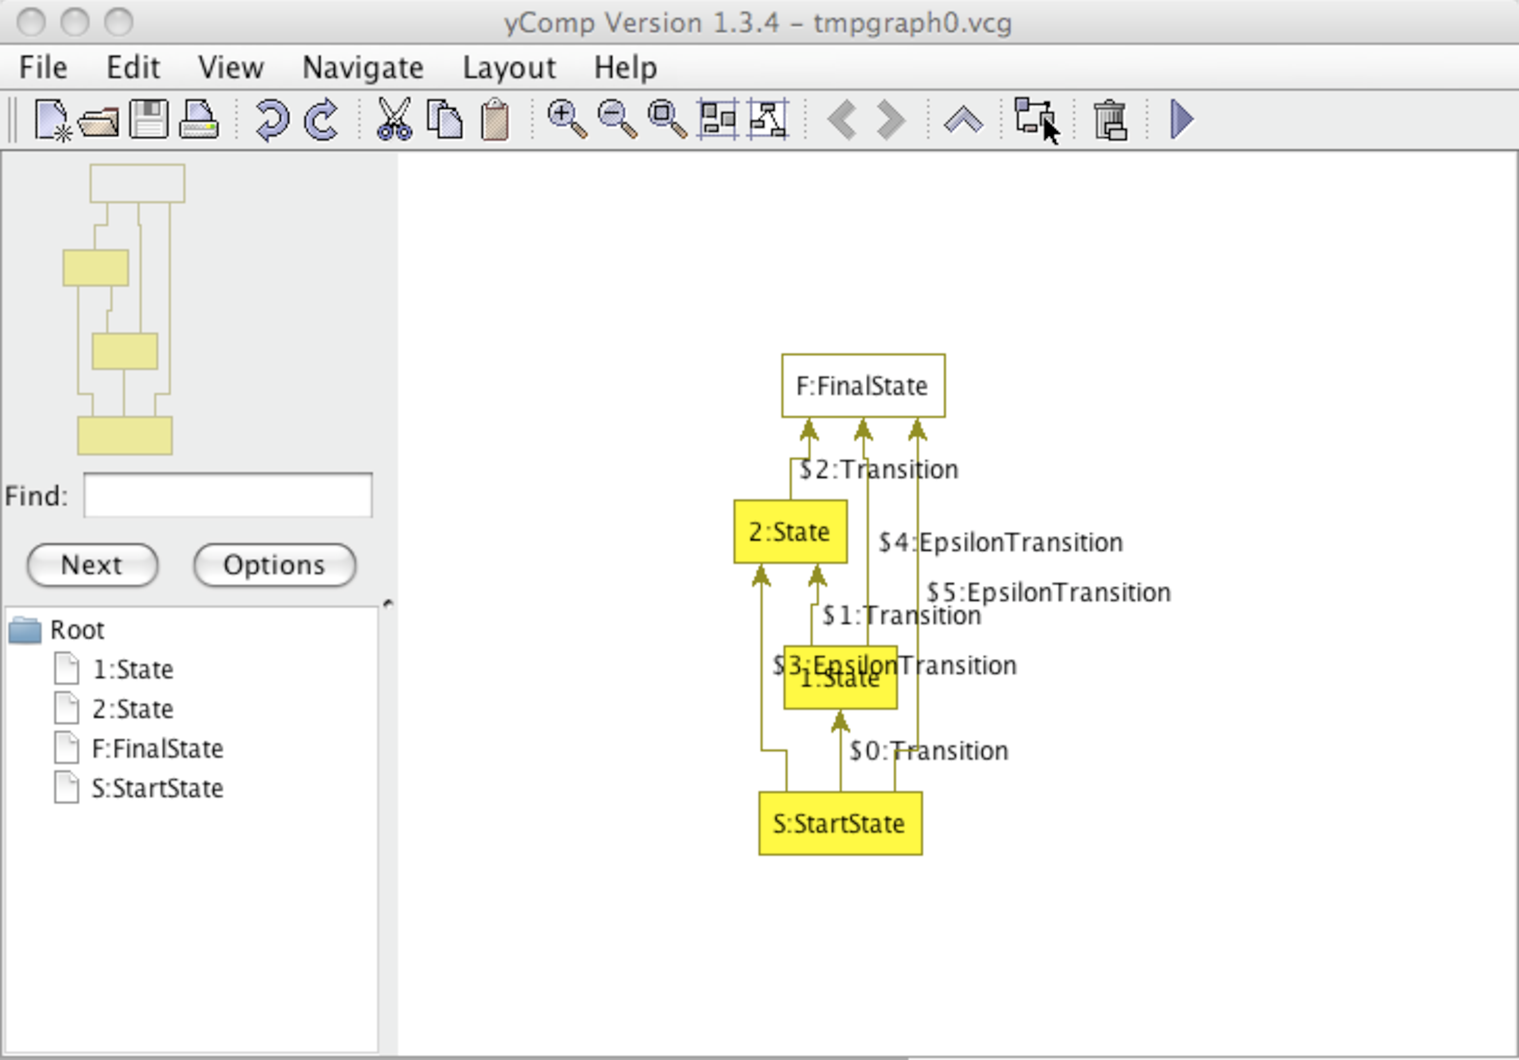
\includegraphics[width=0.8\linewidth]{fig/quickycomp}
	\caption{A first state machine}
	\label{fig:quick:ycomp}
\end{figure}
The graph looks still a bit confusing.
In fact it is quite normal that \yComp's automatic layout algorithm needs manual adjustments.
Quit \yComp\ and exit the \GrShell\ by typing \texttt{exit}.

This script starts with creating an empty graph of the meta model \texttt{StateMachine} (which is referenced by the rule set \texttt{remove\_epsilons.grg}) with the name \texttt{StateMachineGraph}.
Thereafter we create nodes and edges.
The double point notation indicates a node or edge type.
Also note the inplace-arrow notation for edges (\texttt{-Edge->} resp.\ \texttt{-:EdgeType->}).
As you can see, attributes of graph elements can be set during creation with a call-like syntax.
\makeatletter
The \texttt{\$} and \texttt{@} notation is due to the fact that we have two kinds of ``names'' in the \GrShell.
Namely we have \emph{shell variables}---which we did not use, no shell variable is explicitly defined in this script---and \emph{persistent names} that denote a specific graph element.
Persistent names are set by \texttt{\$=Identifier} on creation and accessed by \texttt{@(Identifier)}.
\makeatother
The quote chars around \texttt{"1"} and \texttt{"2"} are used to type these characters as (identifier) strings rather than numbers.

\section{The Rewrite Rules}
We will now add the actual rewrite rules to the rule set file \texttt{remove\_epsilons.grg}.
The idea is to ``forward'' the $\varepsilon$-transitions one after another, i.e.\ if we have a pattern like \texttt{a:State -EpsilonTransition-> b:State -e:Transition-> c:State} we forward to \texttt{a -e-> c}.
After all such transitions are forwarded we can remove the $\varepsilon$-transitions alltogether.
The complete rule set is shown in figure \ref{fig:quick:ruleset}.
See chapter \ref{chaprulelang} for the rule set language reference.
\begin{figure}[htbp]
	\centering
	\begin{grgen}
using state_machine;

test CheckStartState {
    x: StartState;
    negative {
        x;
        y: StartState;
    }
}

test CheckDoublettes {
    negative {
        x:State -e:Transition-> y:State;
        hom(x,y);
        x -doublette:Transition-> y;
        if { typeof(doublette) == typeof(e); }
        if { ((typeof(e) == EpsilonTransition) || (e.Trigger == doublette.Trigger)); }
    }
}

rule ForwardTransition {
    x:State -:EpsilonTransition-> y:State -e:Transition-> z:State;
    hom(x,y,z);
    negative {
        x -exists:Transition-> z;
        if { typeof(exists) == typeof(e); }
        if { ((typeof(e) == EpsilonTransition) || (e.Trigger == exists.Trigger)); }
    }
    modify {
        x -forward:typeof(e)-> z;
        eval { forward.Trigger = e.Trigger; }
    }    
}

rule AddStartFinalState {
    x:StartState -:EpsilonTransition-> :FinalState;
    modify {
        y:StartFinalState<x>;
        emit ("Start state (" + x.id +  ") mutated into a start-and-final state");
    }
}

rule AddFinalState {
    x:State -:EpsilonTransition-> :FinalState;
    if { typeof(x) < SpecialState; }
    modify {
        y:FinalState<x>;
    }
}

rule RemoveEpsilonTransition {
    -:EpsilonTransition->;
    replace {}   
}	
	\end{grgen}
	\caption{Rule set for removing $\varepsilon$-transitions}
	\label{fig:quick:ruleset}
\end{figure}

In detail: The rule set file consists of a number of rules and tests, each of them has a name, like \texttt{ForwardTransition}.
Rules contain a pattern expressed as several semicolon-separated pattern statements and a modify part or a rewrite part.
Tests contain only a pattern; they are used to check for a certain pattern without doing any rewrite operations.
If a rule is applied, \GrG\ tries to find the pattern within a host graph, for instance within the graph we created in section \ref{sct:quick:create}.
Of couse there could be several matches for a pattern---\GrG\ will choose one of them arbitrarily.

Figure \ref{fig:quick:ruleset} also shows the syntax \texttt{x:NodeType} for nodes and \texttt{-e:EdgeType->} for Edges, as we have already seen it in section \ref{sct:quick:create}.
There are also statements like \texttt{:FinalState} or \texttt{-:EpsilonTransistion->}, i.e.\ we are searching for a node of type \texttt{FinalState} resp.\ an edge of type \texttt{EpsilonTransition}, but we are not assigning these graph elements to a name (like \texttt{x} or \texttt{e} above).
Such a defining of names is a key concept of the \GrG\ rule sets: names work as connection points between several pattern statements and between the pattern and the replace / modify part.
As a general rule: If you want to do something with your found graph element, define a name; otherwise an anonymous graph element will do fine.
Also have a look at example \ref{ex:somegraphlets} on page \pageref{ex:somegraphlets} for additional pattern specifications.
The difference between a replace part and a modify part is that a replace part deletes every graph element of the pattern which is not explicitly mentioned in the replace part.
The modify part deletes nothing (by default), but just adds or adjusts graph elements.

What else can we do? 
We have negative application conditions (NACs), expressed by \texttt{negative \{\dots\}}; this prevents a rule to be applicated if the negative pattern is found.
We also have boolean conditions, expressed by \texttt{if \{\dots\}}; a rule is only applicable if all such conditions hold true.
Note, the dot notation to access attributes (as in \texttt{e.Trigger}).
The \texttt{emit} statement prints a string to \texttt{stdout}.
The \texttt{hom(x,y)} and \texttt{hom(x,y,z)} statements mean ``match the embraced nodes homomorphically'', i.e.\ they can actually be matched to the same node within the host graph.
The \texttt{eval \{\dots\}} statement is used to recalculate attributes of graph elements.
Have a look at the statement \texttt{y:StartFinalState<x>} in \texttt{AddStartFinalState}: we \emph{retype} the node \texttt{x}.
That means the newly created node \texttt{y} is actually the node \texttt{x} (including its incident edges and attribute values) except for the node type which is changed to \texttt{StartFinalState}.
Imagine retyping as kind of a type cast.

Now that we have the rules as rewrite primitives we have to compose them to a sequence of rules.
For instance we don't want to forward just one $\varepsilon$-transition as \texttt{ForwardTransition} would do; we want to forward them all.
Such a rule composing is done by a \emph{graph rewrite sequence} (see section \ref{sct:xgrs}).
We add the following line to our shell script \texttt{remove\_epsilons.grs}:
\begin{grgen}
debug xgrs (CheckStartState && CheckDoublettes) && <ForwardTransition* | AddStartFinalState | AddFinalState* | RemoveEpsilonTransition*>
\end{grgen}
This looks like a boolean expression and in fact it behaves similar.
The whole expression is evaluated from left to right.
A rule is successful evaluated if a match could be found.
We first check for a valid state machine, i.e.\ if the host graph has exactly one start state and no redundant transitions.
Thereafter we do the actual rewriting.
These three steps are connected by lazy-evaluation-ands (\texttt{\&\&}), i.e.\ if one of them fails the evaluation will be canceled.
We continue by disjunctive connected rules (connected by \texttt{|}).
The angle brackets (\texttt{<>}) around the transformation rules indicate transactional processing: If the enclosed sequence returns \texttt{false} for some reason, all the already performed graph operations will be rolled back.
That means not all of the rules must find a match.
The \texttt{*} is used to apply the rule repeatedly as long as a match can be found.
This includes applying the rule zero times.
Even in this case \texttt{Rule*} is still successful.

\section{Debugging and Output}
If you execute the modified \GrShell\ script, \GrG\ starts its debugger.
This way you can follow the evaluation of the graph rewrite sequence step by step in \yComp.
Just play around with the keys \texttt{d}, \texttt{s}, and \texttt{r} in \GrShell: the \texttt{d} key lets you follow a single rewrite operation in multiple steps; the \texttt{s} key jumps to the next rule; and the \texttt{r} key runs to the end of the graph rewrite sequence.
Finally you should get a graph like the one in figure \ref{fig:quick:final}
\begin{figure}[htbp]
	\centering
	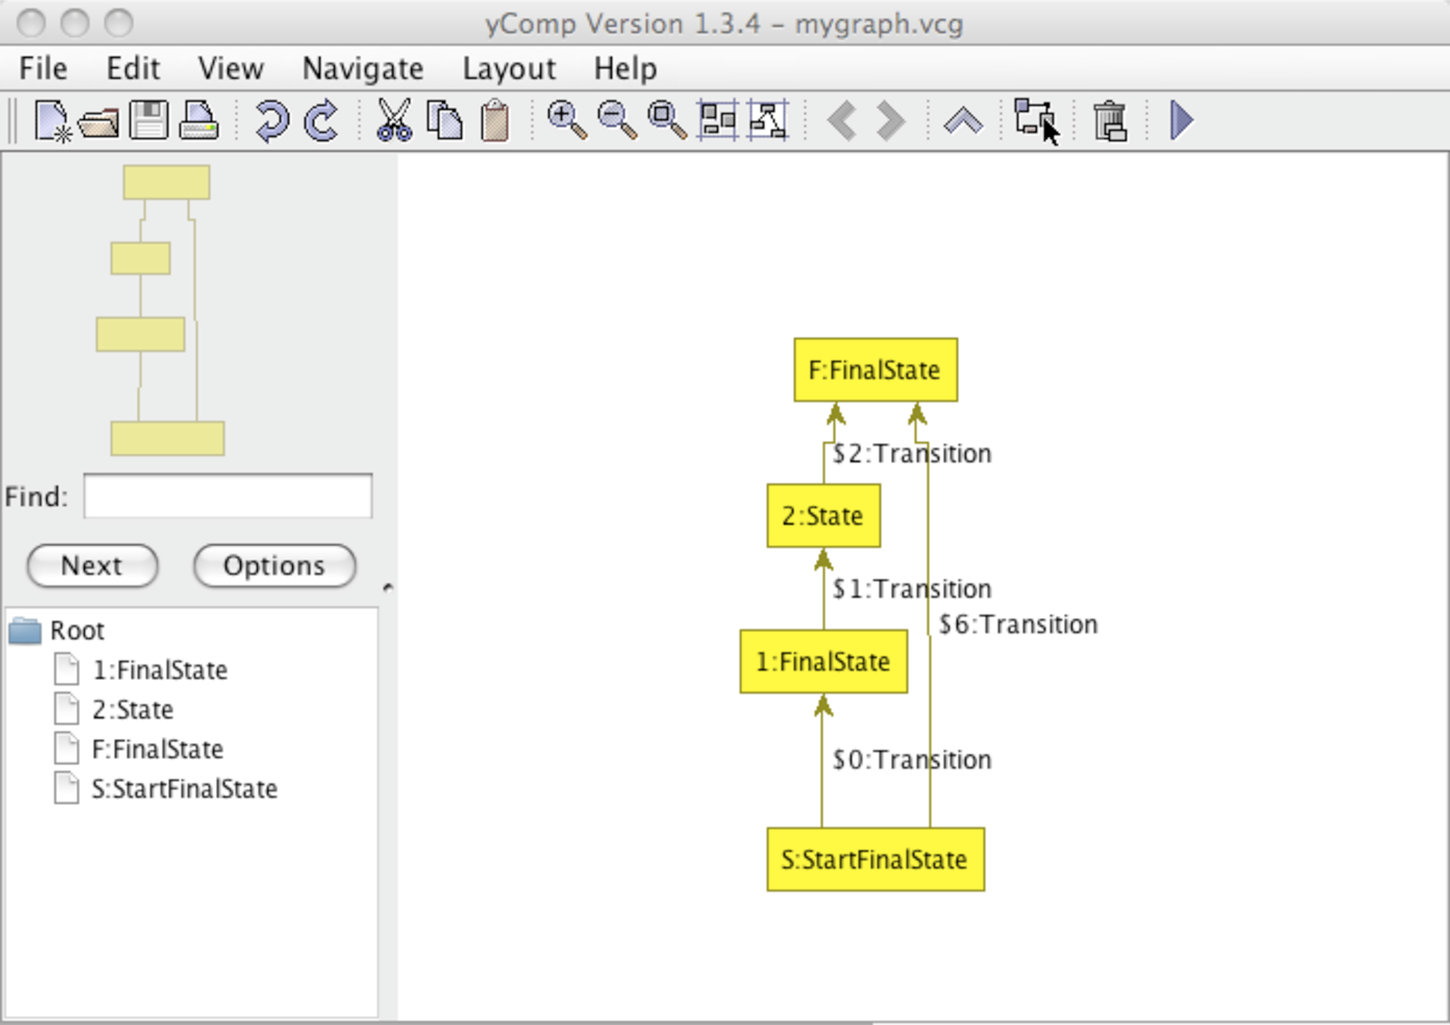
\includegraphics[width=0.8\linewidth]{fig/quickfinal}
	\caption{A state machine without $\varepsilon$-transitions}
	\label{fig:quick:final}
\end{figure}

If everything is working fine you can delete the \texttt{debug} keyword in front of \texttt{xgrs}.
Maybe you want to save the resulting graph.
This is possible by typing \texttt{dump graph mygraph.vcg} in the \GrShell.
\GrShell\ writes the graph in \texttt{mygraph.vcg} into the current directory.
Files in VCG format are readable by \yComp.
Feel free to browse the \texttt{examples} folder shiped with \GrG\ and have a look at further capabilities of the software.


\chapter{Graph Model Language}\indexmain{graph model language}
\label{chapmodellang}
The key features of \GrG\ \emph{graph models}\indexmain{graph model} as described by Geiß et al. \cite{GBGHS:06,KG:07}:

\begin{description}
\item[Types] Nodes and edges are typed. 
  This is similar to classes in common programming languages, except for the concept of methods that \GrG\ nodes and edges don't support. 
\item[Attributes] Nodes and edges can possess attributes. The set of attributes assigned to a node or edge is determined by its type. The attributes themselves are typed, too.
\item[Inheritance] Node and edge types (classes) can be composed by multiple \indexed{inheritance}. \texttt{Node} and \texttt{Edge} are built-in root types of node and edge types, respectively. Inheritance eases the specification of attributes because subtypes inherit the attributes of their super types. Note that \GrG\ lacks a concept of overwriting. On a path in the \indexed{type hierarchy} graph from a type up to the built-in root type there must be exactly one declaration for each attribute identifier. Furthermore if multiple paths from a type up to the built-in root type exist, the declaring types for an attribute identifier must be the same on all such paths.
\item[Connection Assertions] To specify that certain edge types should only connect specific nodes, we include connection assertions. Furthermore the number of outgoing and incoming edges can be constrained.
\end{description}

\begin{figure}[htbf]
\begin{example}\label{ex:model:map}
The following toy example of a model of road maps gives a rough picture of the language:
\begin{grgen}
model Map;

enum resident {village = 500, town = 5000, city = 50000}

node class sight;

node class city {
	size: resident;
}

const node class metropolis extends city {
  river: string;
}  

abstract node class abandoned_city extends city;
node class ghost_town extends abandoned_city;

edge class street;
edge class trail extends street;
edge class highway extends street
    connect metropolis [+] -> metropolis [+]
{
    jam: boolean;
}
\end{grgen}
\end{example}
\end{figure}
In this chapter as well as in chapter \ref{chapgrshell} (\GrShell) we use excerpts of example~\ref{ex:model:map} (the \texttt{Map} model) for illustration purposes.

\section{Building Blocks}
\label{modelbb}

\begin{note}
The following syntax specifications make heavy use of \newtermsee{syntax diagram}{rail diagram}s (also known as \indexed{rail diagram}s). Syntax diagrams provide a visualization of EBNF\footnote{Extended Backus–Naur Form.} grammars. Follow a path along the arrows through a diagram to get a valid sentence (or sub sentence) of the language. Ellipses represent terminals whereas rectangles represent non-terminals. For further information on syntax diagrams see \cite{MMJW:91}.
\end{note}
Basic elements of the \GrG\ graph model language are identifiers to denominate types, attributes, and the model itself. The \GrG\ graph model language is \indexed{case sensitive}.\\
\\
\emph{Ident}, \emph{IdentDecl}\\ \indexmain{identifier}\nopagebreak
A non-empty character sequence of arbitrary length consisting of letters, digits, or underscores. The first character must not be a digit. \emph{Ident} and \emph{IdentDecl} differ in their role: While \emph{IdentDecl} is a \emph{defining} occurrence of an identifier, \emph{Ident} is a \emph{using} occurrence. An \emph{IdentDecl} non-terminal can be annotated\indexmain{annotation}. See \ref{annotations} for annotations of declarations.
\begin{note}
\label{note:modeldecl}
  The \GrG\ model language does not distinguish between \indexed{declaration}s and \indexed{definition}s. More precisely, every declaration is also a definition. For instance, the following C-like pseudo \GrG\ model language code is illegal:
\begin{grgen}
node class t_node;
node class t_node {
  ...
}
\end{grgen}
Using an identifier before defining it is allowed. Every used identifier has to be defined exactly once.
\end{note}
\mbox{ }\\
\emph{NodeType}, \emph{EdgeType}, \emph{EnumType}\\ \nopagebreak
These are (semantic) specializations of \emph{Ident} to restrict an identifier to denote a node type, an edge type, or an enum type, respectively.

\section{Type Declarations}
\begin{rail}
  GraphModel: 'model' IdentDecl ';' (() + TypeDeclaration);
\end{rail}\ixkeyw{model}\ixnterm{GraphModel}
The \indexed{graph model} consists of its name \emph{IdentDecl} and type declarations defining specific node and edge types as well as enums.

\begin{rail}
  TypeDeclaration: EnumDeclaration | ClassDeclaration
\end{rail}\ixnterm{TypeDeclaration}
\emph{ClassDeclaration} defines a node type or an edge type. \emph{EnumDeclaration} defines an enum type for use as attribute of nodes or edges. Like all identifier definitions, types do not need to be declared\indexmain{declaration} before they are used.

\begin{rail}
  EnumDeclaration: 'enum' IdentDecl lbrace ((IdentDecl (() | '=' IntExpr)) + ',') rbrace ;
\end{rail}\ixkeyw{enum}\ixnterm{EnumDeclaration}
Defines an \indexed{enum type}.

\begin{example}
\begin{grgen}
enum Color {red, green, blue}
enum Resident {village = 500, town = 5000, city = 50000}
enum AsInC {a = 2, b, c = 1, d, e = (int)Resident::village + c}
\end{grgen}
The semantics is as in C \cite{Sch:1990:ANSIC}. So, the following holds: $\texttt{red} = 0$, $\texttt{green} = 1$, $\texttt{blue} = 2$, $\texttt{a}=2$, $\texttt{b}=3$, $\texttt{c}=1$, $\texttt{d}=2$, and $\texttt{e}=501$.
\end{example}

\begin{rail}  
  ClassDeclaration: (() | 'abstract') (() | 'const') (NodeClass | EdgeClass);
\end{rail}\ixkeyw{abstract}\ixkeyw{const}\ixnterm{ClassDeclaration}
Defines a new node type or edge type. The keyword \texttt{abstract} indicates that you cannot instantiate graph elements of this type. Instead you have to derive non-abstract types to create graph elements. The abstract-property will not be inherited by subclasses, of course.

\begin{example}
We adjust our map model and make \texttt{city} abstract:
\begin{grgen}
abstract node class city {
	size: int;
}
abstract node class abandoned_city extends city;
node class ghost_town extends abandoned_city;
\end{grgen}
You will be able to create nodes of type \texttt{ghost\_town}, but not of type \texttt{city} or \texttt{abandoned\_city}. However, nodes of type \texttt{ghost\_town} are also of type \texttt{abandoned\_city} as well as of type \texttt{city} and they have the attribute \texttt{size}, hence.
\end{example}
The keyword \texttt{const} indicates that rules may not write to attributes (see also section \ref{replacepart}, \texttt{eval}). However, such attributes are still writable by \LibGr\indexmain{libGr} and \GrShell\indexmain{GrShell} directly. This property applies to attributes defined in the current class, only. It does not apply to inherited attributes. The \texttt{const} property will not be inherited by subclasses, either. If you want a subclass to have the \texttt{const} property, you have to set the \texttt{const} modifier explicitly.

\begin{rail}  
  NodeClass: 'node' 'class' IdentDecl (() | 'extends' (NodeType+',')) \\ 
    (';' | lbrace AttributeDeclarations rbrace);
\end{rail}\ixkeyw{node}\ixkeyw{class}\ixkeyw{extends}\ixnterm{NodeClass}
Defines a new \indexed{node type}. Node types can inherit\indexmain{inheritance} from other node types defined within the same file. If the \texttt{extends} clause is omitted, \emph{NodeType} will inherit from the built-in type \texttt{\indexed{Node}}. Optionally nodes can possess attributes.

\begin{rail}    
  EdgeClass: 'edge' 'class' IdentDecl (() | 'extends' (EdgeType+',')) \\
    (() + ConnectAssertions) (';' | lbrace AttributeDeclarations rbrace);
\end{rail}\ixkeyw{edge}\ixkeyw{class}\ixkeyw{extends}\ixnterm{EdgeClass}
Defines a new \indexed{edge type}. Edge types can inherit\indexmain{inheritance} from other edge types defined within the same file. If the \texttt{extends} clause is omitted, \emph{EdgeType} will inherit from the built-in type \texttt{\indexed{Edge}}. Optionally edges can possess attributes. A \newterm{connection assertion} specifies that certain edge types should only connect specific nodes and, moreover, the number of outgoing and incoming edges can be constrained.

\begin{note}
It is not forbidden to create graphs that are invalid according to \indexed{connection assertion}s. \GrG\ just enables you to check, whether a graph is valid or not. See also section \ref{graphcommands}, \texttt{validate}.
\end{note}

\begin{rail}  
  ConnectAssertions: 'connect' (NodeConstraint '->' NodeConstraint + ',');
  NodeConstraint: NodeType (() | '[' ('*' | '+' | Number | RangeConstraint) ']') ;
  RangeConstraint: Number ':' ('*' | Number) ;
\end{rail}\ixkeyw{connect}\ixnterm{ConnectAssertions}\ixnterm{NodeConstraint}\ixnterm{RangeConstraint}
A \indexed{connection assertion} is denoted as a pair of node types in conjunction with their multiplicities\indexmainsee{multiplicity}{connection assertion}. A corresponding edge may connect a node of the first node type or one of its subtypes (source) with a node of the second node type or one of its subtypes (target). The multiplicity is a constraint on the out-degree and in-degree\indexmainsee{degree}{connection assertion} of the source and target node type, respectively. \emph{Number} is an \texttt{int} constant as defined in section \ref{expressions}. See \ref{graphcommands}, \texttt{validate}\ixkeyw{validate}, for an example. Table \ref{multiplicities} describes the multiplicity definitions.
\begin{table}[htbp]
\begin{tabularx}{\linewidth}{|l|X|}\hline
	\texttt{[$n$:*]} & The number of edges, nodes of that type are incident to, is unbounded. At least $n$ edges must be incident to nodes of that type.\\ 
	\texttt{[$n$:$m$]} & At least $n$ edges must be incident to nodes of that type, but at most $m$ edges may be incident to nodes of that type ($m \geq n$ must hold).\\
	\texttt{[*]} & Abbreviation for \texttt{[0:*]}.\\
	\texttt{[+]} & Abbreviation for \texttt{[1:*]}.\\
	\texttt{[$n$]} & Abbreviation for \texttt{[$n$:$n$]}. \\ \hline
\end{tabularx}
\caption{\GrG\ node constraint multiplicities}
\label{multiplicities}
\end{table}

\begin{rail}    
  AttributeDeclarations: (() | IdentDecl ':' AttributeType ';') + ;
  AttributeType: PrimitiveType | EnumType ; 
\end{rail}\ixnterm{AttributeDeclarations}\ixnterm{AttributeType}
Defines a node or edge \indexed{attribute}. Possible types are enumeration types (\texttt{enum}) and primitive types. See section~\ref{builtin} for a list of built-in primitive types.





\chapter{Rule Set Language}
\label{chaprulelang}

The rule set language forms the core of \GrG. Rule files refer to zero\footnote{Omitting a graph model means that \GrG\ uses a default graph meta model. The default model consists of the base type \texttt{Node} for vertices and the base type \texttt{Edge} for edges.} or more graph models and specify a set of rewrite rules. The rule language covers the pattern specification and the replace/modify specification. Attributes of graph elements can be re-evaluated during a rule application. The following rewrite rule by Geiß et al. \cite{geiss} gives a rough picture of the language:
%\begin{figure}[tb]
\begin{example}\label{ex:rule:SomeRule}
\begin{grgen}
actions SomeActions using SomeModel;

rule SomeRule {
  pattern {
    n1 : NodeTypeA;
    n2 : NodeTypeA;
    hom(n1, n2);
    n1 --> n2; /*@\label{ex:somerule:graphlet}@*/
    n3: NodeTypeB;
    negative {
      n3 -e1:EdgeTypeA-> n1;
      if {n3.a1 == 42*n2.a1;}
    }
    negative { /*@\label{ex:somerule:secondnac:begin}@*/
      n4: Node \ (NodeTypeB);
      n3 -e1:EdgeTypeB-> n4;
      if {typeof(e1) >= EdgeTypeA;}
    } /*@\label{ex:somerule:secondnac:end}@*/
  }
  replace {
    n5: NodeTypeC<n1>;
    n3 -e1:EdgeTypeB-> n5;
    eval {
      n5.a3 = n3.a1*n1.a2;
    }
  }  
}
\end{grgen}
\end{example}
%\end{figure}
In this chapter we use excerpts of example~\ref{ex:rule:SomeRule} (\texttt{SomeRule}) for illustration purposes.

\section{Building Blocks}
\label{rulebb}

The \GrG\ rule set language is case sensitive. The language makes use of several identifier specializations in order to denominate all the \GrG\ entities.\\
\\
\emph{Ident}, \emph{IdentDecl}\\ \nopagebreak
A non-empty character sequence of arbitrary length consisting of letters, digits or underscores. The first character must not be a digit. \emph{Ident} may be an identifier defined in a graph model (see \ref{modelbb}). \emph{Ident} and \emph{IdentDecl} differ in their role: While \emph{IdentDecl} is a \emph{defining} occurrence of an identifier, \emph{Ident} is a \emph{using} occurrence. An \emph{IdentDecl} non-terminal can be annotated. See \ref{annotations} for annotations of declarations.
\begin{note}
  The \GrG\ rule set language does not distinguish between declarations and definitions. More precisely, every declaration is also a definition. That means, that every element of a LHS (left hand side, see section \ref{patternpart}) is actually mapped by a match. 
\end{note}
\mbox{ }\\
\emph{ModelIdent}, \emph{TypeIdent}, \emph{NodeType}, \emph{EdgeType}\\
These are (semantic) specializations of \emph{Ident}. \emph{TypeIdent} matches every type identifier, i.e. a node type, an edge type, an enum type or a primitive type. All the type identifiers are actually type \emph{expressions}. See \ref{typeexpressions} for the use of type expressions.\\

\begin{rail}
  Graphlet: (GraphletNode (() | Continuation) | Continuation) ';' ;
  Continuation: GraphletEdge (() | (GraphletNode (() | Continuation))) ;
\end{rail}
A graphlet specifies a connected subgraph. 
By graphlets \GrG\ provides a descriptive notation to define both, patterns to search for as well as the subgraphs that replace or modify matched spots in a host graph. 
A graph is specified piecewise by graphlets. 
In example \ref{ex:rule:SomeRule}, line \ref{ex:somerule:graphlet}, the statement \texttt{n1 --> n2} is the node identifier \texttt{n1} followed by the continuation graphlet \texttt{--> n2}.

All the graph elements of a graphlet have got a \emph{name}.
The name is either user assigned or an unique internal, non-accessible name.
In the second case the graph element is called \emph{anonymous}.
For illustration purposes we use a \texttt{\$<number>} notation to denote anonymous graph elements in this document.
Names may not be redefined; once defined, a name is \emph{bound} to a graph element. 
We use the term ``binding of names'' because a name not only denote a graph element of a graphlet, but also denotes the mapping of the abstract graph element of a graphlet to a concrete graph element of a host graph.
So graph elements of different names are pairwise distinct except for homomorphically matched graph elements (see section \ref{patternpart}).\\
For instance \texttt{v:NodeType1 -e:EdgeType-> w:NodeType2} selects some node of type \texttt{Node\-Type1} that is connected to a node of type \texttt{NodeType1} by an edge of type \texttt{EdgeType} and binds the names \texttt{v}, \texttt{w}, and \texttt{e}. 
If \texttt{v} and \texttt{w} are not explicitly marked as homomorphic, they are distinct.\\
Binding of names allows for splitting a single graphlet into multiple graphlets as well as defining cyclic structures.
\begin{example}
The following graphlet (\texttt{n1}, \texttt{n2}, and \texttt{n3} are defined somewhere else)
\begin{grgen}
n1 --> n2 --> n3 <-- n1;
\end{grgen}
is equivalent to
\begin{grgen}
n2 --> n3;
n1 --> n2;
n3 <-- n1;
\end{grgen}
and \texttt{n1 --> n3} is equivalent to \texttt{n3 <-- n1}, of course.
\end{example}
The visibility of names is determined by scopes. 
Scopes can be nested. 
Names of surrounding scopes are visible in inner scopes. 
Usually a scope is defined by \texttt{\{} and \texttt{\}}.
In terms of scopes the replace part is a direct inner scope of the pattern part.
In example \ref{ex:rule:SomeRule} the negative condition from lines \ref{ex:somerule:secondnac:begin} to \ref{ex:somerule:secondnac:end} uses \texttt{n3} from the surrounding scope and defines \texttt{n4} and \texttt{e1}. 
We may safely reuse the variable name \texttt{e1} in the replace part.

\begin{rail}
GraphletNode: (Ident | 
    '.' |
    (() | IdentDecl) ':' NodeType (() | TypeConstraint | '<' Ident '>')) ;   
\end{rail}
Specifies a node of type \emph{NodeType} with respect to \emph{TypeConstraint} (see section \ref{typeexpressions}, \emph{TypeConstraint}). 
Type constraints are allowed in the pattern part only. 
The \texttt{.}\ is an anonymous node of the base type \texttt{Node}. 
Remember that every node type has \texttt{Node} as super type. The \texttt{<>} operator retypes a node. Retyping is allowed in the replace/modify part only (see section \ref{replacepart}, \emph{Retyping}).
\begin{center}
  \begin{tabular}[c]{ll}
    \textbf{Graphlet} & \textbf{Meaning}\\ \hline
    \texttt{x:NodeType;} & The name \texttt{x} is bound to a node of type \texttt{NodeType} or one of its subtypes. \\
    \texttt{ :NodeType;} & \texttt{\$1:NodeType} \\
    \texttt{.;} & \texttt{\$1:Node} \\
    \texttt{x;} & The node \texttt{x} is bound to.
  \end{tabular}
\end{center} 

\begin{rail}
  GraphletEdge: '-' (() | EdgeRefinement) '->'  | '<-' (() | EdgeRefinement) '-' ;
  EdgeRefinement: Ident | (() | IdentDecl) ':' EdgeType (() | TypeConstraint | '<' Ident '>') ;
\end{rail}
Specifies an edge. Anonymous edges are specified by \texttt{-->} or \texttt{<--}. For a more detailed specification you can use an inplace notated edge refinement clause. Type constraints are allowed in the pattern part only (see section \ref{typeexpressions}, \emph{TypeConstraint}). The \texttt{<>} operator retypes an edge. Retyping is allowed in the replace/modify part only (see section \ref{replacepart}, \emph{Retyping}).\\
\begin{center}
  \begin{tabular}[c]{ll}
    \textbf{Graphlet} & \textbf{Meaning}\\ \hline
    \texttt{ -e:EdgeType-> ;} & The name \texttt{e} is bound to an edge of type \texttt{EdgeType} or one of its subtypes  \\
    \texttt{ -:EdgeType-> ;} & \texttt{ -\$1:EdgeType-> ;} \\
    \texttt{ --> ;} & \texttt{ -\$1:Edge-> ;} \\
    \texttt{ -e-> ;} & The edge \texttt{e} is bound to.
  \end{tabular}
\end{center} 
As the above table shows, edges can be defined and used separately, i.e.\ without their incident nodes. Beware of accidentally redirecting an edge: 
The graphlets
\begin{grgenlet}
-e:Edge-> .;
x:Node -e-> y:Node;
\end{grgenlet}
are illegal, because they would effect redirecting of edge \texttt{e}. 
However, the graphlets
\begin{grgenlet}
x:Node -e:Edge-> y:Node;
 -e-> ;
\end{grgenlet}
are allowed, but the second graphlet is pointless. In particular the second graphlet does not identify or create any ``copies'', neither occurring in the pattern part nor occurring in the replace part.
\begin{example}
Some attempts to specify a loop edge:\\
\mbox{ }\\
\begin{tabular}[c]{ll} 
 \textbf{Graphlet} & \textbf{Meaning} \\ \hline
 \texttt{x:Node -e:Edge-> x;} & The edge \texttt{e} is a loop.\\ 
 \texttt{x:Node -e:Edge-> ; -e-> x;} & The edge \texttt{e} is a loop.\\ 
 \texttt{-e:Edge-> x:Node;} & The edge \texttt{e} may or may not be a loop.\\ 
 \texttt{.\ -e:Edge-> .;} & The edge \texttt{e} is certainly not a loop.\\ 
\end{tabular}
\end{example}

\begin{figure}[htbp]
\begin{example}
Some graphlets:

\begin{center}
\begin{tabular}[c]{cl}
  & \\
  \begin{tabular}[c]{c}\begin{tikzpicture}
      \tikzstyle{every node}=[circle]
      \node[draw] (n1) at (1,0) {};
      \node[draw] (n2) at (2,1) {};
      \node[draw] (n3) at (1,2) {};
      \node[draw] (n4) at (0,1) {};
    	
      \draw[-latex] (n3) .. controls +(-1,0) .. (n4) {};
      \draw[-latex] (n4) .. controls +(0,-1) .. (n1) {};
      \draw[-latex] (n1) .. controls +(1,0) .. (n2) {};
      \draw[-latex] (n2) .. controls +(0,1) .. (n3) {};
    \end{tikzpicture}\end{tabular} & \begin{tabular}[c]{l} \texttt{x:Node --> .\ --> .\ --> .\ --> x;} \end{tabular}\\
  & \\  
  \begin{tabular}[c]{c}\begin{tikzpicture}
      \tikzstyle{every node}=[circle]
      \node[draw] (n1) at (1,1) {};
      \node[draw] (n2) at (0,0) {};
      \node[draw] (n3) at (0,2) {};
      \node[draw] (n4) at (2,0) {};
      \node[draw] (n5) at (2,2) {};
    	
      \draw[-latex] (n1) -- (n2) {};
      \draw[-latex] (n1) -- (n3) {};
      \draw[-latex] (n1) -- (n4) {};
      \draw[-latex] (n1) -- (n5) {};
    \end{tikzpicture}\end{tabular} & \begin{tabular}[c]{l} \texttt{.\ <-- x:Node --> .;} \\ \texttt{.\ <-- x --> .;} \end{tabular}\\
  & \\
  \begin{tabular}[c]{c}\begin{tikzpicture}
      \tikzstyle{every node}=[circle]
      \node[draw] (n1) at (3,5) {};
      \node[draw] (n2) at (2,4)   {};
      \node[draw] (n3) at (0,2)   {};
      \node[draw] (n4) at (2,0)   {};
      \node[draw] (n5) at (4,2)   {};
      \node[draw] (n6) at (2,5.0)   {};
    	
    	\draw[-latex] (n2) --                                  (n1) node[right,pos=0.6] {$e_1:\text{stem}$};
    	\draw[-latex] (n2) .. controls +(-1,1) and +(0,1) ..   (n3) node[left,midway]  {$e_2$};
      \draw[-latex] (n3) .. controls +(0,-1) and +(-1,0) ..  (n4) node[left,midway]  {$e_3$};
    	\draw[-latex] (n4) .. controls +(1,0)  and +(0,-1) ..  (n5) node[right,midway] {$e_4$};
      \draw[-latex] (n5) .. controls +(0,1)  and +(1,1) ..   (n2) node[right,midway] {$e_5$};
    	\draw[-latex] (n2) .. controls +(-0.3,+0.3) and +(-0.3,-0.3) .. (n6) node[left,midway]   {};
    	\draw[-latex] (n2) .. controls +(+0.3,+0.3) and +(+0.3,-0.3) .. (n6) node[right,midway]  {};
    \end{tikzpicture}\end{tabular} & \begin{tabular}[c]{l} \texttt{.\ <-e1:stem- n1:Node -e2:Edge-> .\ -e3:Edge-> .} \\ \quad\texttt{-e4:Edge-> .\ -e5:Edge-> n1;}\\ \texttt{n1 --> n2:Node;} \\ \texttt{n1 --> n2;} \end{tabular}\\
   & \\
  \begin{tabular}[c]{c}\begin{tikzpicture}
      \tikzstyle{every node}=[circle]
      \node[draw] (n1) at (0,0) {};
      \node[draw] (n2) at (1,0) {};
      \node[draw] (n3) at (2,0) {};
      \node[draw] (n4) at (3,0) {};
      \node[draw] (n5) at (4,0) {};
    	
      \draw[-latex] (n1) -- (n2) {};
      \draw[-latex] (n3) -- (n2) {};
      \draw[-latex] (n4) -- (n3) {};
      \draw[-latex] (n4) -- (n5) {};
    \end{tikzpicture}\end{tabular} & \begin{tabular}[c]{l} \texttt{.\ --> .\ <-- .\ <-- .\ --> .;} \end{tabular}
\end{tabular}\\
\end{center}
\mbox{ }\\
\mbox{ }\\
\mbox{ }\\
And some illegal graphlets:\\
\mbox{}\\
\mbox{}\\
\begin{tabularx}{\linewidth}{cX}
\texttt{-e:Edge-> ; .\ -e-> .;} & Would effect redirecting of edge \texttt{e}. \\
 & \\
 \texttt{x -e:T-> y; x -e-> x;} & Would effect redirecting of edge \texttt{e}. \\
  & \\
 \texttt{x:Node; negative \{y:Node; hom(x,y)\}} & Here \texttt{x} must not occur in the \texttt{hom} statement. See section \ref{patternpart} for further information. \\
  & \\
  \texttt{<-- --> ;} & There must be at least a node between the edges.
\end{tabularx}
\end{example}
\end{figure}

\begin{note}
Although both, the pattern part and the replace/modify part, use graphlets, there are subtle differences between them. It concerns the \emph{TypeConstraint} clause, the retype operator \texttt{<>}, and the scope of defined graph element names: Names defined within the pattern part are valid in the pattern part as well as in the replace/modify part. Names defined within the replace/modify part are unknown to the pattern part.
\end{note}

\section{Rules and Tests}
\label{ruledecls}
The structure of a rule set file is as follows:
\begin{rail}
  'actions' IdentDecl (() | 'using' ((ModelIdent)+',')) ';' \\ ((TestDeclaration | RuleDeclaration)+) ;
\end{rail}
A rule set consists of the underlying graph models and several rewrite rules. In case of multiple graph models \GrG\ uses the union of these models. In this case beware of conflicting declarations. There is no built-in conflict resolution mechanism like packages or namespaces for models. If necessary you could use prefixes as you might do it in C.

\begin{rail}
  TestDeclaration: 'test' ActionSignature lbrace Pattern rbrace ;
  RuleDeclaration: 'rule' ActionSignature lbrace Pattern Replace rbrace ;
\end{rail}
Declares a single rewrite rule such as \texttt{SomeRule}. It consists of a pattern part (see \ref{patternpart}) in conjunction with its rewrite/modify part (see \ref{replacepart}). A \emph{test} has no rewrite specification. It's intended to check whether (and maybe how many times) a pattern occurs.
\begin{example}
We define a test \texttt{SomeCond}
\begin{grgen}
test SomeCond {
  pattern {
    n: SeldomNodeType;
  }
}
\end{grgen}
and execute in \GrShell:
\begin{grshell}
  grs SomeCond & SomeRule
\end{grshell}
SomeRule will only be executed, if a node of type \texttt{SeldomNodeType} exists. For regular graph rewrite sequences in \GrShell\ see \ref{grsthings}.
\end{example}

\begin{rail}  
  ActionSignature: IdentDecl (() | Parameters) (() | ':' ReturnTypes) ;
\end{rail}
The signature sets the name of a rewrite rule to \emph{IdentDecl} and optionally names and types of formal parameters as well as a list of return types. Parameters provide users with the ability to pass graph elements to and from a rule. This is similar to parameters of procedural languages.

\begin{rail}
  Parameters: '(' ((IdentDecl ':' NodeType | '-' IdentDecl ':' EdgeType '->') + ',') ')' ;
  ReturnTypes: '(' ((NodeType | EdgeType) + ',') ')' ;
\end{rail}
Within a rule parameters are treated as (predefined) graph elements of the pattern. Even if a supplied parameter value is undefined, it is treated as valid node or edge definition. So in any case a graph element of the specified type has to be mapped. \GrG\ assumes the lookup operation for parameters to be in $\mathcal{O}(1)$. In case of an undefined parameter value this might lead to bad search plans, because \GrG\ has to actually search for such a graph element.
\begin{example}
Assume the following rule:
\begin{grgen}
rule r(-e:Edge->; x:Node) {
  pattern {
    x --> ;
    negative {
      <-- x -->;
    }
  }
  modify {}
}
\end{grgen}
If \texttt{x} and \texttt{e} are undefined, rule \texttt{r} is equivalent to rule \texttt{s}:
\begin{grgen}
rule s {
  pattern {
    x:Node --> ;
    -e:Edge-> ;
    negative {
      <-- x -->;
    }
  }
  modify {}
}
\end{grgen}
In particular \texttt{x} will not be incident to \texttt{e}.
\end{example}
The return types specify edge and node types of graph elements that are returned by the replace/modify part. If return types are specified, the \texttt{return} statement is mandatory. Otherwise no \texttt{return} statement must occur. See also section \ref{replacepart}, \texttt{return}.
\begin{example}
We extend \texttt{SomeRule} with a variable node to find and we want it to return the rewritten graph elements \texttt{n5} and \texttt{e1}.
\begin{grgen}
  rule SomeRuleExt(varnode: Node): (Node, EdgeTypeB) {
    pattern {
      n1: NodeTypeA;
      ...
    }
    replace {
      varnode;
      ...  
      return(n5, e1);
      eval {
        ...
\end{grgen}
We don't define \texttt{varnode} within the pattern part because this is already covered by the parameter specification itself.
\end{example}

\section{Pattern Part}
\label{patternpart}
\begin{rail}
  Pattern: 'pattern' lbrace (()+PatternStatement) rbrace ;
\end{rail}
A pattern consists of zero or more pattern statements. All the pattern statements must be fulfilled by a subgraph of the host graph in order to form a match. Even stronger -- a graph element of the host graph, that is matched by a statement, is \emph{bound}, i.e.\ it cannot be part of another pattern statement, unless you use the \texttt{hom} operator. An empty pattern always produces exactly one (empty) match. This is caused by the uniqueness of the totally undefined function.\\
Pattern statements may define names for graph elements for use by other pattern statements or replace statements. Such names may be used before their declaration. See section \ref{rulebb} for a detailed explanation of names and graphlets.
\begin{note}
The application of a rule is not deterministic (remember the introducing example in \ref{ov:example}), in particular there may be more than one subgraph that matches the pattern. 
Whereas the \GrShell\ selects one of them arbitrarily (without further abilities to control the selection), the underlying \LibGr\ provides a mechanism to deal with such ambiguities. 
\LibGr\ allows for splitting a rule application into two steps: Find all the subgraphs of the host graph that matches the pattern and rewrite one of this matches. 
By returning a collection of all matches, the \LibGr\ retains the complete graph rewrite process under control.
As a \LibGr\ user use the following methods of the \texttt{IAction} interface:
\begin{csharplet}
IMatches Match(IGraph graph, int maxMatches, IGraphElement[] parameters);
IGraphElement[] Modify(IGraph graph, IMatch match);
\end{csharplet}
This might look like this in C\#:
\begin{csharplet}
IMatches myMatches = myAction.Match(myGraph, -1, null); /* -1: get all the matches */
for (int i = 0;  i < myMatches.NumMatches; i++)
{
	if (inspectCarefully(myMatches.GetMatch(i))
	{
		myAction.Modify(myGraph, myMatches.GetMatch(i));
		break;
  	}
}
\end{csharplet}

Also notice that the regular graph rewrite sequences introduces a further variant of indeterminism on rule application level: 
The \texttt{\$<op>} flag marks the operator \texttt{<op>} as commutative, i.e.\ the execution order of its operands (rules) is indeterministic. 
See section \ref{grsthings} for further information on regular graph rewrite sequences.
\end{note}

\begin{rail}  
  PatternStatement: 
    Graphlet ';' |
    'hom' '(' (Ident + ',') ')' ';' |
    'negative' lbrace (()+PatternStatement) rbrace |
    'if' lbrace (BooleanExpr ';' +) rbrace |
    'return' '(' (Ident+',') ')' ';' ;
\end{rail}
The semantics of the various pattern statements:
\begin{description}
  \item[Graphlet.] Graphlets specify connected subgraphs. See section \ref{rulebb} for a detailed explanation of graphlets. 
  \item[Isomorphic/Homomorphic Matching.] The \texttt{hom} operator specifies the nodes or edges that may be matched homomorphically. In contrast to the default isomorphic matching, the specified graph elements \emph{may} be mapped to the same graph element in the host graph. Note that the graph elements shall have a common supertype. Several homomorphically matched graph elements will be mapped to a graph element of a common supertype.\\
  In example \ref{ex:rule:SomeRule} node \texttt{n1} and node \texttt{n2} may be the same node. This is possible because they are of the same type (\texttt{NodeTypeA}).\\
  The \texttt{hom} operator is transitive, i.e.\ \texttt{hom(a, b); hom(b, c);} implies \texttt{hom(a, c);}. 
  Inside a NAC the \texttt{hom} operator may only operate on graph elements that are either defined or used in the NAC.
  \item[Negative Application Conditions (NACs).] With negative application conditions (keyword \texttt{negative}) we can specify graph patterns which forbid the application of a rule if any of them is present in the host graph (cf. \cite{adam}). 
  NACs must not be nested.
  NACs possess an own scope. 
  Names defined within a NAC are not alive outside the NAC. 
  Identifiers from surrounding scopes may be overwritten.
  In general NACs does not care about bindings within the outer scope. 
  Nevertheless, if you use an identifier that is defined in the outer scope, this specifies exactly the graph element, the identifier is bound to in the outer scope.
  \begin{example}
    We specify a node \texttt{x} with out-degree 2:
    \begin{grgen}
pattern {
  <-- x:Node -->;
  negative {
    <-- x -->;
    x -->;
  }
}
    \end{grgen}
  \end{example}
  \item[Attribute Conditions.] The Java-like attribute conditions (keyword \texttt{if}) in the pattern part allow for further restriction of the applicability of a rule.
  \item[Return values.] The return statement is only allowed for tests. Otherwise the \texttt{return} statement belongs to the replace part. See \ref{replacepart}, \emph{Return Values}.
\end{description}
Keep in mind that using type constraints or the \texttt{typeof} operator might be helpful. See section \ref{typeexpressions} for further information.

\section{Replace/Modify Part}
\label{replacepart}
For the task of rewriting \GrG\ provides two different modes: A replace mode and a modify mode.
\begin{description}
  \item[Replace mode.] The semantics of this mode is to delete every graph element of the pattern that is not used (denoted) in the replace part, keep every graph element that is used, and create every additionally defined graph elements. ``Using'' means using a graph element in a graphlet. Attribute calculations are no using occurrences.\\
  In example \ref{ex:rule:SomeRule} \texttt{SomeRuleExt} the nodes \texttt{varnode} and \texttt{n3} will be kept. The node \texttt{n1} is replaced by the node \texttt{n5} preserving \texttt{n1}'s edges. The anonymous edge instance between \texttt{n1} and \texttt{n2} only occurs in the pattern and therefore gets deleted.
  \item[Modify mode.] The modify mode can be regarded as a replace part in replace mode, where every pattern graph element is added (denoted) before the first replace statement. In particular even the anonymous graph elements are kept. Additionally this mode supports the \texttt{delete} operator that deletes every element given as an argument. Deletion takes place after all other rewrite operations. Multiple deletion of the same graph element is allowed (but pointless) as well as deletion of just created elements (pointless, too).
\begin{example}
How might example \ref{ex:rule:SomeRule} look in modify mode? We have to denominate the anonymous edge between \texttt{n1} and \texttt{n2} in order to delete it. The node \texttt{varnode} should be omitted. So we have
\begin{grgen}
rule SomeRuleModify {
  pattern {
    ...
    n1 -e0:Edge-> n2;
    ...
  }
  modify {
    n5 : NodeTypeC<n1>;
    n3 -e1:EdgeTypeB-> n5;
    delete(e0);
    eval {
      ...
\end{grgen}
\end{example}
\end{description}

\begin{rail}
  Replace: ('replace' | 'modify') lbrace (()+ReplaceStatement) rbrace ;
\end{rail}
Selects whether the replace mode or the modify mode is used. Several replace statements describe the transformation from the pattern subgraph to the destination subgraph.

\begin{rail}  
  ReplaceStatement: Graphlet ';' |
    'delete' '(' (Ident + ',') ')' ';' |
    'eval' lbrace (Assignment ';' +) rbrace |
    'return' '(' (Ident+',') ')' ';' ;
\end{rail}    
The semantics of the various pattern statements:
\begin{description}
  \item[Graphlet.] Analogous to a pattern graphlet, a specification of a connected subgraph. Its graph elements are either kept because they are elements of the pattern or added otherwise. Names defined in the pattern part must not be redefined in the replace graphlet. See section \ref{rulebb} for a detailed explanation of graphlets. 
  \item[Deletion.] The \texttt{delete} operator is only available in the modify mode. It deletes the specified pattern graph elements. Multiple occurrences of \texttt{delete} statements are allowed. Deletion statements are executed after all other replace statements. Multiple deletion of the same graph element is allowed (but pointless) as well as deletion of just created elements (pointless, too).
  \item[Attribute Evaluation.] If a rule is applied, then the attributes of matched and inserted graph elements will be recalculated.
  \item[Return Values.] Graph elements of the replace/modify part can be returned according to the return types in the signature (see \ref{ruledecls}, \texttt{ActionSignature}). The \texttt{return} statement must not occur multiple times. The graph element names have to be in the same order as the corresponding return types in the signature. The named elements must be compatible to the declared type.
  \item[Retyping.] Retyping enables us to keep all adjacent nodes and all attributes stemming from common super types of a graph element while changing its type. Retyping differs from a type cast: During replacement both of the graph elements are alive. Specifically both of them are available for evaluation. Furthermore the source and destination types need not to be on a path in the directed type hierarchy tree, rather their relation can be arbitrary.\\
The edge specification as well as \emph{ReplaceNode} supports retyping. In example \ref{ex:rule:SomeRule} node \texttt{n5} is a retyped node stemming from node \texttt{n1}.
\end{description} 

\begin{rail}    
   Assignment: Ident '.' Ident '=' Expression ;
\end{rail}
Several evaluation parts are allowed within the replace part. Multiple evaluation statements will be internally concatenated, preserving their order. Evaluation statements have imperative semantics. In particular, \GrG\ does not care about data dependencies. Evaluation takes place before any graph element gets deleted and after all the new elements have been created. You may read (and write, although this doesn't make sense) attributes of graph elements to be deleted.
\begin{example}
\begin{grgen}
...
modify {
  ...
  eval {y.i = 40;}
  eval {y.j = 0;}
  x: IJNode;
  y: IJNode;
  delete(x);
  eval {
    x.i = 1; 
    y.j = x.i;
    x.i = x.i + 1;
    y.i = y.i + x.i;
  }
\end{grgen}
This nonsense example yields $\texttt{y.i} = 42$, $\texttt{y.j} = 1$.
\end{example}



\chapter{Nested and Subpatterns}\indexmain{rule set language nested and subpatterns}
\label{cha:nestedsub}

The extension of the rule set language described in the previous chapter by nested patterns and subpatterns greatly enhances the flexibility and expressiveness of pattern matching and rewriting.
The following patterns to match a simplified abstract syntax tree give a rough picture of the language of nested and subpatterns:
  \begin{example}
    \begin{grgen}
test method
{
  m:Method <-- n:Name; // signature of method consisting of name
  iterated { // and 0-n parameters
    m <-- :Variable;
  }  
  
  :AssignmentList(m); // body consisting of a list of assignment statements
}

pattern AssignmentList(prev:Node)
{
  optional { // nothing or a linked assignment and again a list
    prev --> a:Assign; // assignment node 
    a -:target-> v:Variable; // which has a variable as target 
    :Expression(a);  // and an expression which defines the left hand side 
    :AssignmentList(a); // next one, plz
  }
}

pattern Expression(root:Expr)
{
  alternative { // expression may be
    Binary { // a binary expression of an operator and two expresions
      root <-- expr1:Expr;
	  :Expression(expr1);
      root <-- expr2:Expr;
	  :Expression(expr2);
      root <-- :Operator;
    }
    Unary { // or a unary expression which is a variable (reading it)
      root <-- v:Variable;
    }
  }
}
    \end{grgen}
  \end{example}\label{introexample}


Until now we have seen rules and tests with one left hand side static pattern specification in a direct 1:1 correspondence with its dynamic match in the host graph on a successful application.
From now on we will increase the expressiveness of the pattern language, and dependent on it the rewrite language, to describe much finer and more flexible what patterns to accept.
This will be done by pattern specifications built up from multiple static pattern piece specifications, where the pieces may be matched dynamically zero, one, or multiple times, or are forbidden to exists for the entire pattern to be matched.
These rule set language constructs can be split into nested patterns (negative application condition, positive application condition, nested pattern with cardinality, alternative patterns) and subpatterns (subpattern declaration and subpattern entity declaration, subrule declaration and usage), we will start with the nested patterns:

\begin{rail}  
  NestedPattern: 
    NegativeApplicationCondition |
    PositiveApplicationCondition |
    NestedPatternWithCardinality |
    AlternativePatterns 
    ;
\end{rail}\ixnterm{NestedPattern}

\section{Negative Application Condition (NAC)}
\indexmain{negative application condition}\indexmainsee{NAC}{negative application condition}\label{nac}

\begin{rail}  
  NegativeApplicationCondition: 
    'negative' lbrace (()+PatternStatement) rbrace;
\end{rail}\ixkeyw{negative}\ixnterm{NegativeApplicationCondition}

With negative application conditions (keyword \texttt{negative}) we can specify graph patterns which forbid the application of a rule if any of them is present in the host graph (cf.~\cite{adam}). 
NACs possess a \indexed{scope} of their own, i.e. names defined within a NAC do not exist outside the NAC. 
Identifiers from surrounding scopes must not be redefined.
If they are not explicitely mentioned, the NAC gets matched independent from them, i.e. elements inside a negative are \texttt{hom(everything from the outside)} by default.
But referencing the element from the outside within the negative pattern causes it to get matched isomorphically/distinct to the other elements in the negative pattern. 
This is a bit unintuitive if you think of extending the pattern by negative elements, but cleaner and more powerful: 
just think of NACs to simply specify a pattern which should not be in the graph, with the possibility of forcing elements to be the same as in the enclosing pattern by name equality.

  \begin{example}
    We specify a variable which is not badly typed, i.e. a node \texttt{x} of type \texttt{Variable} which must not be target of an edge of type \text{type} with a source node of type \texttt{BadType}:
    \begin{grgen}
  x:Variable;
  negative {
    x <-:type- :BadType;
  }
    \end{grgen}
  \end{example}
 
Because NACs have their ``own'' binding, using NACs leads to specifications which might look a bit redundant.

  \begin{example}
    Let's check the singleton condition, meaning there's exactly one node of the type to check, for the type \texttt{RootNamespace}.
    The following specification is \emph{wrong} (it will never return a match):
    \begin{grgen}
  x:RootNamespace;
  negative {
    y:RootNamespace;
  }
    \end{grgen}
	
    Instead we have to specify the \emph{complete} forbidden pattern inside the NAC. This is done by:
    
	\begin{grgen}
  x:RootNamespace;
  negative {
    x;
    y:RootNamespace; // now it is ensured that y must be different from x
  }
    \end{grgen}
	
	Btw: the \texttt{x;} is not a special construct, it's a normal graphlet (cf. \ref{sct:graphlets}).
	
  \end{example} 

If there are several patterns which should not occur, use several negatives.
If there are exceptions to the forbidden pattern, use nested negatives.
As a straight-forward generalization of negatives within positive patterns, negatives may get nested to an arbitrary depth.
Matching of the nested negative pattern causes the matching of the nesting pattern to fail.

\begin{example}
  A fabricated example using parallel as well as nested \texttt{negative}s:
  \begin{grgen}
test onlyOneChildOrAllChildrenHaveExactlyOneCommonChild
{
  root:Class;
  negative {
    root -:extending-> :Class; // root does not extend another class
  }
  root <-:extending- c1:Class; // a class c1 extends root
  negative {
    c1;
    root <-:extending- c2:Class; // there is no c2 which extends root
    negative {
      c1 <-:extending- child:Class -:extending-> c2; // except c1 and c2 have a common child
	  negative { // and c1 has no further children
	    child;
	    c1 <-:extending- :Class;
	  }
	  negative { // and c2 has no further children
	    child;
	    c2 <-:extending- :Class; 
	  }
    }
  }
}
  \end{grgen}
\end{example}

%negative pattern elements get matched independent from the subpatterns utilizing them
%(explicit patternpath/pattern statement in the negative/independent needed for old behaviour)

	
\section{Positive Application Condition (PAC)}
\indexmain{positive application condition}\indexmainsee{PAC}{positive application condition} \label{pac}

\begin{rail}  
  PositiveApplicationCondition: 
    'independent' lbrace (()+PatternStatement) rbrace;
\end{rail}\ixkeyw{independent}\ixnterm{PositiveApplicationCondition}

With positive application conditions (keyword \texttt{independent}) we can specify graph patterns which, in contrast to negative application conditions, must be present in the host graph to cause the matching of the enclosing pattern to succeed.
Together with NACs they share the property of opening a \indexed{scope}, with elements being independent from the surrounding scope (i.e. a host graph element can easiely get matched to a pattern element and a PAC element with a different name, unless the pattern element is referenced in the PAC). 
They are used to improve the logical structure of rules by separating a pure condition from the main pattern of the rule amenable to rewriting.
They are really needed if subpatterns want to match elements which were already matched during the subpattern derivation.

\begin{example}
  A further fabricated example rather giving the intention using \texttt{independent} patterns to check some conditions with only the main pattern available to rewriting:

  \begin{grgen}
rule moveMethod
{
  c:Class --> m:Method;
  csub -:extending-> c;
  csub:Class -e:Edge-> msub:Method;
  
  independent {
    // a complicated pattern to find out that m and msub have same signatures
  }
  independent {
    // a complicated pattern to find out that msub is only using variables available in c
  }
  independent {
    // a complicated pattern to find out that m is not used
  }
 
  modify { // move method upwards
    delete(m);
    delete(e);
    c --> msub;
  }
}
  \end{grgen}
\end{example}

  
\section{Pattern Cardinality}
\indexmainsee{cardinality}{pattern cardinality}\indexmain{pattern cardinality}\label{cardinality}

\begin{rail}  
  NestedPatternWithCardinality: 
    ('iterated' | 'multiple' | 'optional') lbrace NestedBody rbrace;
  NestedBody: (PatternStatement+) NestedRewriting?;
\end{rail}\ixkeyw{iterated}\ixkeyw{multiple}\ixkeyw{optional}\ixnterm{NestedPatternWithCardinality}

The \indexmain{pattern cardinality} blocks allow to specify how often the nested pattern -- opening a scope -- is to be matched.
Matching will be carried out eagerly, i.e. if the construct is not limiting the number of matches and a further match is possible it will be done.
(The nested body will be explained in Section~\ref{sec:nestedrewrite}.)

\subsubsection*{The iterated block} 
is matching the contained subpattern as often as possible, succeeding even in the case the contained pattern is not available (thus it will never fail).
It was included in the language to allow for matching breadth-splitting structures, as in capturing all methods of a class in a program graph.

\begin{example}
  \begin{grgen}
test methods
{
  c:Class;
  iterated {
    c --> m:Method;
  }  
}
  \end{grgen}
\end{example}

\subsubsection*{The multiple block}
is working like the iterated block, but expects the contained subpattern to be available at least once, if it is not, matching of the multiple block and thus its enclosing pattern fails.

\begin{example}
  \begin{grgen}
test oneOrMoreMethods
{
  c:Class;
  multiple {
    c --> m:Method;
  }
}
  \end{grgen}
\end{example}

\subsubsection*{The optional block}
is working like the iterated block, but matches the contained subpattern at most once, further occurences of the subpattern are left unmatched.
If the nested pattern is available, it will get matched, otherwise it won't; matching of the optional block will succeed either way.

\begin{example}
  \begin{grgen}
test variableMaybeInitialized
{
  v:Variable; // match variable
  optional { // and an initialization with a different one if available
    v <-- otherV:Variable;
  }
}
  \end{grgen}
\end{example}

\begin{note}
Pattern cardinality constructs are match/rewrite-all enumeration blockers.
For every pattern instance, the iterated/... yields only one match, even if in all mode.
\end{note} 


\section{Alternative Patterns}
\indexmain{alternative patterns}\label{alternative}

\begin{rail}  
  AlternativePatterns: 
    'alternative' lbrace ((CaseName lbrace NestedBody rbrace)+()) rbrace;
\end{rail}\ixkeyw{alternative}\ixnterm{AlternativePattern}

With the alternative block you can specify several nested alternative patterns. One of them must get matched for the matching of the alternative (and thus its directly nesting pattern) to succeed, and only one of them is matched per match of the alternative / overall pattern.
The order of matching the alternative patterns is unspecified, especially it is not guaranteed that a case gets matched before the case textually following -- if you want to ensure that a case can not get matched if another case could be matched, you must explicitely prevent that from happening by adding negatives to the cases.
In contrast to the iterated which locally matches everything available and inserts this combined match into the current match, the alternative decides for one case match which it inserts into the current match tree, ignoring other possible matches by other cases. 

\begin{example}
  \begin{grgen}
test feature(c:Class)
{
	alternative // a feature of the class is either
	{
		FeatureMethod { // a method
			c --> :Method;
		}
		FeatureVariable { // or a variable
			c --> :Variable;
		}
		FeatureConstant { // or a constant
			c ---> :Constant;
		}
	}
}  
  \end{grgen}
\end{example}

\begin{example}
  \begin{grgen}
test variableMaybeInitialized
{
  v:Variable; // match variable
  alternative { // and an initialization with a different one if available
    Empty {
        // the empty pattern matches always	
	  negative { // so prevent it to match if initialization is available
        v <-- otherV:Variable;
	  }
	}
	Initialized { // initialization
      v <-- otherV:Variable;
	}
  }
}
  \end{grgen}
\end{example}

\section{Subpattern Declaration and Subpattern Entity Declaration}
\indexmain{subpattern}\label{sec:subpattern}

Subpatterns were introduced to factor out a common recurring pattern -- a shape -- into a named subpattern type, ready to be reused at points the pattern should get matched.
The common recurring pattern is specified in a subpattern declaration and used by a subpattern entity declaration.

\begin{rail}  
  SubpatternDeclaration: 
    'pattern' IdentDecl Parameters? (('modify'|'replace') Parameters)? \\
	lbrace SubpatternBody rbrace ;
  SubpatternBody: (PatternStatement+) SubpatternRewriting?;
\end{rail}\ixkeyw{pattern}\ixkeyw{modify}\ixkeyw{replace}\ixnterm{SubpatternDeclaration}\ixnterm{SubpatternBody}\label{subpatterndecl}\indexmain{subpattern declaration}

Subpattern declarations define a subpattern type denoting the specified shape in global namespace; the parameters specify some context elements the pattern may refer to, but which are not part of the pattern itself. 
So they are only syntactically the same as test/rule-parameters (which are members of the pattern part), a further difference is the lack of ReturnTypes, due to the fact that a subpattern can't return anything (they are not actions, just a helper in constructing complex patterns).
Subpatterns can receive additional rewrite parameters in contrast to the actions; they can be used to hand in elements which are created in the rewrite part of the action or subpattern which contains the subpattern entity.
(The nested body will be explained in Section~\ref{sec:subrule}.)

\begin{rail}  
  SubpatternEntityDeclaration: 
    Ident ':' SubpatternType '(' ')' ';' ;
\end{rail}\ixnterm{SubpatternEntityDeclaration}\indexmain{subpattern entity declaration}

Subpattern entity declarations instantiate an entity of the subpattern type (i.e. specified shape), which means the subpattern must get matched for the matching of the enclosing pattern to succeed.
The arguments given are bound to the corresponding parameters of the subpattern.
If you prefer a syntactical point of view, you may see the subpattern entity as a placeholder, which gets substituted in place by the textual body of the subpattern declaration under renaming of the parameters to the arguments.

%TODO:remove
%Termersetzung mit Termen die Graphen beschreiben.
%Mehrelementige Graphsprachen als Zwischenschritt zu den rekursiven bereits mit alternative... eingef�hrt -- dort auch so erkl�rt, wirklich eingef�hrt? vor rekursiv trotzdem noch ein  Zwischenschritt: pattern mit alternative, statt action mit alternative

\begin{example}
  \begin{grgen}
pattern TwoParameters(mp:Method)
{
  mp <-- :Variable;
  mp <-- :Variable;
}
test methodAndFurther
{
  m:Method <-- n:Name;
  tp:TwoParameters(m);
}
  \end{grgen}

  In the given example a subpattern \texttt{TwoParameters} is declared, connecting the context element \texttt{mp} via two edges to two variable nodes.
  The test \texttt{methodAndFurther} is using the subpattern via the declaration of the entity \texttt{tp} of type \texttt{TwoParameters}, binding the context element to its local node \texttt{m}.
  The resulting test after subpattern derivation is equivalent to the test \texttt{methodWithTwoParameters}.

  \begin{grgen}
test methodWithTwoParameters
{
  m:Method <-- n:Name;
  m <-- :Variable;
  m <-- :Variable;
}
  \end{grgen}
\end{example}


\subsection{Recursive Patterns}\indexmain{recursive pattern}\indexmain{structural recursion}

Subpatterns can be combined with alternative patterns or the cardinality patterns into recursive subpatterns, i.e. subpatterns which may contain themselves.
Subpatterns containing themselves alone -- directly or indirectly -- would never yield a match.

\begin{example}
  \begin{grgen}
test iteratedPath
{
  root:Assign;
  negative { --> root; }
  :IteratedPath(root); // match iterated path = assignment list
}

pattern IteratedPath(prev:Node)
{
  optional { // nothing or a linked assignment and again a list
    prev --> a:Assign; // assignment node 
    :IteratedPath(a); // next one, plz
  }
}
  \end{grgen}
  
Searches an iterated path from the root node on, here an assinment list. 
The iterated path with the optional is equivalent to the code below (note the negative which ensures you get a longest match -- without it the empty case may be chosen lazily just in the beginning)
  
  \begin{grgen}
pattern IteratedPath(prev:Node)
{
  alternative {
    Empty {
      negative {
        prev --> a:Assign;
      }
    }
    Further {
      prev --> a:Assign;
      :IteratedPath(a);
    }
  }
}
  \end{grgen}
\end{example}


\begin{example}
  \begin{grgen}
rule removeMiddleAssignment
{
  a1:Assign --> a2:Assign --> a3:Assign;
  independent {
    :IteratedPath(a1,a3)
  }
  
  replace {
    a1; a3;
  }
}

pattern IteratedPath(begin:Assign, end:Assign)
{
  alternative { // an iterated path from begin to end is either
    Found { // the begin assignment directly linked to the end assignment (base case)
      begin --> end;
    }
    Further { // or an iterated path from the node after begin to end (recursive case)
      begin --> intermediate:Assign;
      :IteratedPath(intermediate, end);
    }
  }
}
  \end{grgen}

This is once more a fabricated example, for an iterated path from a source node to a distinctive target node, and an example for the interplay of subpatterns and positive application conditions to chech complex conditions independent from the pattern already matched.
Here, three nodes \texttt{a1},\texttt{a2},\texttt{a3} of type \texttt{Assign} forming a list connected by edges are searched, and if found, \texttt{a2} gets deleted, but only if there is an iterated path of directed edges from \texttt{a1} to \texttt{a3}.
The path may contain the host graph node matched to \texttt{a2} again.
Without the \texttt{independent} this would not be possible, as all pattern elements -- including the ones originating from subpatterns -- get matched isomorphically. 
The same path specified in the pattern of the rule -- not in the independent -- would not get matched if it would go through the host graph node matched to b, as it is locked by the isomorphy constraint.

\end{example}

With recursive subpatterns you can altready capture neatly structures extending into depth (as iterated paths)
and also structures extending into breadth (as forking patterns, although the cardinality statements are often better suited to this task).
But combined with an iterated block, you may even match structures extending into breadth and depth,
like e.g. a hierarchy of classes (i.e. match a spanning tree(todo:indexed) in the graph)
giving you a very powerful and flexible notation to capture large, complex patterns
built up in a stuctured way from simple, connected pieces (as e.g. abstract syntax trees of programming languages).

\begin{example}
  \begin{grgen}
pattern SpanningTree(root:Class)
{
  iterated {
    root <-:extending- next:Class;
    :SpanningTree(next);
  }
}
  \end{grgen}
\end{example}


\section{Nested Pattern Rewriting}
\indexmain{nested pattern rewrite}\label{sec:nestedrewrite}

Until now we focused on the pattern matching of nested and subpatterns -- but we're not only interested in finding patterns combined from several pattern pieces, we want to rewrite the pattern pieces, too.
This does not hold for the application conditions, which are pure conditions, but for all the other language constructs introduced in this chapter.

\begin{rail}  
  NestedRewriting: ('replace' | 'modify') lbrace (()+ReplaceStatement) rbrace;
\end{rail}\ixnterm{NestedRewriting}\ixkeyw{replace}\ixkeyw{modify}

Syntactically the rewrite is specified by a modify or replace clause nested directly within the scope of each nested pattern;
in addition to the rewrite clause nested within the top level pattern, which must be present even if the top level pattern is empty. 
Semantically for every instance of a pattern piece matched its dependent rewrite is applied. 
So in the same manner the complete pattern is assembled from pattern pieces, the complete rewrite gets assembled from rewrite pieces
(or operationally: rewriting is done along the match tree by rewriting one pattern piece after the other).
Note that neither \texttt{exec} statements nor \texttt{return} statements are available as in the top level rewrite part of a rule.

For a static pattern specification like the iterated block yielding dynamically a combined match of zero to many pattern matches, every submatch is rewritten, according to the rewrite specification applied to the host graph elements of the match bound to the pattern elements
(if the pattern was matched zero times, no dependent rewrite will be triggered - but note that zero matches still means success for an iterated, so the dependent rewrite piece of the enclosing pattern will be applied).
This allows e.g. for reversing all edges in the iterated-example (denoting containment in the class), as it is shown in the first of the following two examples.
For the alternative construct the rewrite is specified directly at every nested pattern, i.e. alternative case as shown in the second of the following two examples); the rewrite of the matched case will be applied.

Nodes and edges from the pattern containing the nested pattern containing the nested rewrite are not available for deletion inside the nested rewrite;
only the rewrite part of the pattern in which they are declared is allowed to delete them.
They are available for retyping though, but only in case the retyping is unambigous -- it must be guaranteed that only one retyping can occur.
So only the rewrites of alternative cases and optional patterns may contain retypings of elements not declared in the alternative case or optional pattern (in contrast to iterated and multiple pattern rewrites).

\begin{example}
  \begin{grgen}
rule methods
{
  c:Class;
  iterated {
    c --> m:Method;
	
	replace {
	  c <-- m;
	}
  } 

  replace {
    c;
  }  
}
  \end{grgen}
\end{example}

\begin{example}
  \begin{grgen}
rule methodWithTwoOrThreeParameters(m:Method)
{
  alternative {
    Two {
      m <-- n:Name;
      m <-e1:Edge- v1:Variable;
      m <-e2:Edge- v2:Variable;
	  negative {
	    v1; v2; m <-- :Variable;
	  }
	  
	  modify {
	    delete(e1); m --> v1;
	    delete(e2); m --> v2;	    
	  }
	}
	Three {
      m <-- n:Name;
      m <-e1:Edge- v1:Variable;
      m <-e2:Edge- v2:Variable;
      m <-e3:Edge- v3:Variable;
	  
	  modify {
	    delete(e1); m --> v1;
	    delete(e2); m --> v2;
	    delete(e3); m --> v3;
	  }
	}
	
	modify {
	}
}
  \end{grgen}
\end{example}


\section{Subpattern rewriting}
\indexmain{subrule}\label{sec:subrule}

Alongside the separation into subpattern declaration and subpattern entity declaration, subpattern rewriting is separated into a nested rewrite specification given within the subpattern declaration defining how the rewrite looks like and a subpattern rewrite application given withing the rewrite part of the pattern containing the subpattern entity declaration requesting the rewrite to be actually applied.

\begin{rail}  
  SubpatternRewriting: ('replace' | 'modify') lbrace (()+ReplaceStatement) rbrace;
\end{rail}\ixnterm{SubpatternRewriting}\ixkeyw{replace}\ixkeyw{modify}

The subpattern rewriting specifications within the subpattern declaration looks like a nested rewriting specification,
but additionally there may be rewrite parameters given in the subpattern header (cf. \ref{subpatterndecl}) which can be referenced in the rewrite body.
(Most elements can be handed in with normal parametes, but elements created in the rewrite part of the user of the subpattern can only be handed in at rewrite time.) 

\begin{rail}  
  SubpatternRewriteApplication: 
    Ident '(' ((Ident ':' NodeType)*',') ')' ';' |
    SubpatternOccurence |
	'emithere' '(' StringExpr ')' ';'
	;
\end{rail}\ixnterm{SubpatternRewriteApplication}\ixkeyw{emithere}

The SubpatternRewriteApplication is part of a ReplaceStatement.
The subpattern rewrite application is given within the rewrite part of the pattern containing the subpattern entity declaration, in call notation on the declared subpattern identifier.
The \texttt{emithere}-statements are executed before the emit statements, and in the order in between the subpattern rewrite applications they are specified syntactically.

\begin{example}
  \begin{grgen}
pattern TwoParametersAddDelete(mp:Method)
{
  mp <-- v1:Variable;
  mp <-- :Variable;

  modify {
    delete(v1);
    mp <-- :Variable;
  }
}
rule methodAndFurtherAddDelete
{
  m:Method <-- n:Name;
  tp:TwoParametersAddDelete(m);
  
  modify {
    tp(); // trigger rewriting of the TwoParametersAddDelete instance
  }
}
  \end{grgen}
\end{example}


\begin{example}
  \begin{grgen}
pattern IteratedPathReverse(prev:Node)
{
  optional {
    prev --> next:Node;
    ipr:IteratedPathReverse(next);
    
    replace {
    	prev <-- next;
    	ipr();
    }
  }
  
  replace {
  }
}
  \end{grgen}
  Reversing the direction of the edges in an iterated path.
\end{example}

\begin{example}
This is an example for rewrite parameters, connecting every node on an iterated path to a common node (i.e. the local rewrite graph to the containing rewrite graph).
It can't be simulated by subpattern parameters which get defined at matching time because the common element is only created later on, at rewrite time.

  \begin{grgen}
pattern ChainFromToReverseToCommon(from:Node, to:Node) replace(common:Node)
{
  alternative {
    rec {
      from --> intermediate:Node;
      cftrtc:ChainFromToReverseToCommon(intermediate, to);

      replace {
        from <-- intermediate;
        from --> common;
        cftrtc(common);
      }
    }
	base {
      from --> to;

      replace {
        from <-- to;
        from --> common;
        to --> common;
      }
    }
  }

  replace {
    from; to;
  }
}
  \end{grgen}

  \begin{grgen}  
  rule chainFromToReverseToCommon()
  {
    from:Node; to:Node;
	cftrtc:ChainFromToReverseToCommon();
	
	modify {
	  common:Node;
	  cftrtc(common);
	}
  }
  \end{grgen}
\end{example}


\subsection{Deletion and Preservation of Subpatterns}\label{sub:delpressub}

In addition to the fine-grain dependent replacement, subpatterns may get deleted or kept as a whole.

\begin{rail}  
  SubpatternOccurence: 
    Ident ';' |
    'delete' '(' (Ident + ',') ')' ';';
\end{rail}\ixkeyw{SubpatternOccurence}\ixkeyw{delete}

In modify mode, they are kept by default, but deleted if the name of the declared subpattern entity is mentioned within a delete statement.
In replace mode, they are deleted by default, but kept if the name of the declared subpattern entity is mentioned (using occurence, same as with nodes or edges).

\begin{example}
  \begin{grgen}
rule R {
  m1:Method; m2:Method;
  tp1:TwoParameters(m1);
  tp2:TwoParameters(m2);

  replace {
    tp1; // is kept
    // tp2 not included here - will be deleted
    // tp1(); or tp2(); -- would apply dependent replacement
    m1; m2;
  }
}
  \end{grgen}
\end{example}


\section{Regular Expression Syntax}\indexmainsee{EBNF}{regular expression syntax}\indexmain{regular expression syntax}

In addition to the already introduced syntax for the nested patterns with the keywords 
\texttt{negative}, \texttt{independent}, \texttt{alternative}, \texttt{iterated}, \texttt{multiple} and \texttt{optional},
there is a more lightweight syntax resembling regular expressions; 
using it together with the subpatterns gives graph rewrite specifications which look like EBNF-grammars with embedded actions. 
Exceeding the more verbose syntax they offer constructs for matching the pattern a bounded number of times (same notation as the one for the bounded iteration in the xgrs).
Table \ref{keywordregexpsyntax} lists the corresponding (/equivalent) language constructs; 
Example \ref{introexampleregexp} is a version of the introductionary example \ref{introexample} modified to use the new syntax.

\begin{table}[htbp]
  \centering
  \begin{tabularx}{\linewidth}{|l|X|} \hline
    \texttt{ iterated \{ P \} } & \texttt{ (P)* } \\
    \texttt{ multiple \{ P \} } & \texttt{ (P)+ } \\
    \texttt{ optional \{ P \} } & \texttt{ (P)? } \\ 
	\texttt{ alternative \{ l1 \{ P1 \} .. lk \{ Pk \} \} } & \texttt{ (P1|..|Pk) } \\
    \texttt{ negative \{ P \} } & \texttt{ $\sim$(P) } \\
    \texttt{ independent \{ P \} } & \texttt{ \&(P)} \\ \hline 
    \texttt{ modify \{ R \} } & \texttt{  \{+ R \} } \\
    \texttt{ replace \{ R \} } & \texttt{ \{- R \} } \\ \hline 
    \texttt{ - } & \texttt{ (P)[k] / (P)[k:l] / (P)[k:*] } \\ \hline 
	\end{tabularx}
  \caption{Map of nested patterns in keyword syntax to regular expression syntax}
  \label{keywordregexpsyntax}
\end{table}


  \begin{example}
    \begin{grgen}
test method
{
  m:Method <-- n:Name; // signature of method consisting of name
  ( m <-- :Variable; )* // and 0-n parameters
  
  :AssignmentList(m); // body consisting of a list of assignment statements
}

pattern AssignmentList(prev:Node)
{
  ( // nothing or a linked assignment and again a list
    prev --> a:Assign; // assignment node 
    a -:target-> v:Variable; // which has a variable as target 
    :Expression(a);  // and an expression which defines the left hand side 
    :AssignmentList(a); // next one, plz
  )?
}

pattern Expression(root:Expr)
{
  ( // expression may be a binary expression of an operator and two expresions
      root <-- expr1:Expr;
	  :Expression(expr1);
      root <-- expr2:Expr;
	  :Expression(expr2);
      root <-- :Operator;
  | // or a unary expression which is a variable (reading it)
      root <-- v:Variable;
  )
}
    \end{grgen}
  \end{example}\label{introexampleregexp}





\chapter{Types and Expressions}
\label{typeexpr}
In the following sections \emph{Ident} refers to an identifier of the graph model language (see Section~\ref{modelbb}) or the rule set language (see Section~\ref{rulebb}). \emph{TypeIdent} is an identifier of a node type or an edge type, \emph{NodeOrEdge} is an identifier of a node or an edge.

\section{Built-In Types}
\label{builtin}
Besides user-defined node types, edge types, and enumeration types, \GrG\ supports the built-in \indexed{primitive types}\indexmainsee{built-in types}{primitive types} in Table~\ref{builtintypes}.
The exact type format is \indexed{backend} specific. 
The \indexed{LGSPBackend} maps the \GrG\ primitive types to the corresponding C\# primitive types.
\begin{table}[htbp]
\begin{tabularx}{\linewidth}{|l|X|}\hline
	\texttt{\indexed{boolean}} & Covers the values \texttt{true} and \texttt{false} \\
	\texttt{\indexed{int}} & A signed integer with at least 32 bits \\
	\texttt{\indexed{float}}, \texttt{\indexed{double}} & A floating-point number with single precision or double precision respectively \\
	\texttt{\indexed{string}} & A character sequence of arbitrary length\\
	\texttt{\indexed{object}} & Contains a .NET object\\ \hline
\end{tabularx}
\caption{\GrG\ built-in primitive types}
\label{builtintypes}
\end{table}
Table~\ref{tabcasts} lists \GrG's implicit \indexed{type cast}s and the allowed explicit type casts.
Of course you are free to express an implicit type cast by an explicit type cast as well as ``cast'' a type to itself.

According to table~\ref{tabcasts} neither implicit nor explicit casts from {\tt int} to any \indexed{enum type} are allowed.
This is because the range of an enum type is very sparse in general.
For the same reason implicit and explicit casts between enum types are also forbidden.
Thus, enum values can only be assigned to attributes having the same enum type.
A cast of an enum value to a string value will return the declared name of the enum value.
A cast of an object value to a string value will return ``null'' or it will call the \texttt{toString()} method of the .NET object.
Be careful with assignments of objects: \GrG\ does not know your .NET type hierarchy and therefore it cannot check two objects for type compatibility.
Objects of type object are not very useful for \GrG processing, but they can be used on the API level.

\begin{table}[htbp]
  \centering
  \begin{tabular}[c]{|c|ccccccc|} \hline
    \backslashbox{to}{from} & \texttt{enum} & \texttt{boolean} & \texttt{int} & \texttt{float} & \texttt{double} & \texttt{string} & \texttt{object} \\ \hline
    \texttt{enum} & $=$/--- & & & & & & \\ 
    \texttt{boolean} & & $=$ & & & & & \\
    \texttt{int} & implicit & & $=$ & \texttt{(int)} & \texttt{(int)} & & \\
    \texttt{float} & implicit & & implicit & $=$ & \texttt{(float)} & & \\
    \texttt{double} &  implicit & & implicit & implicit & $=$ & & \\
    \texttt{string} & implicit & implicit & implicit & implicit & implicit & $=$ & implicit\\
    \texttt{object} & &  & & & & & $=$ \\\hline
  \end{tabular}
  \caption{\GrG\ type casts}
  \label{tabcasts}
\end{table}

\begin{example}
  \begin{itemize}
    \item Allowed:\\
	  \texttt{x.myfloat = x.myint; x.mydouble = (float) x.myint;\\ x.mystring = (string) x.mybool;}
    \item Forbidden:\\
      \texttt{x.myfloat = x.mydouble;} and \texttt{x.myint = (int) x.mybool;}\\
      \texttt{MyEnum1 = (MyEnum1Type) int;} and \texttt{MyEnum2 = (MyEnum2Type) MyEnum1;}
  where {\tt myenum1} and {\tt myenum2} are different enum types.

  \end{itemize}
\end{example}

\begin{note}
	Unlike an {\tt eval} part (which must not contain assignments to node or edge attributes) the declaration of an enum type can contain assignments of {\tt int} values to \indexed{enum item}s (see section~\ref{typedecl}).
	The reason is, that the range of an enum type is just defined in that context.
\end{note}

TODO: set/map

\section{Expressions}

%left to right, left associative?

\label{expressions}
\begin{rail}
  Expression: BoolExpr | RelationalExpr | IntExpr | FloatExpr | StringExpr | SetExpr | MapExpr | TypeExpr | PrimaryExpr;  
\end{rail}\ixnterm{Expression}


\section{Boolean Expressions}

\begin{rail}
  BoolExpr: ((() | '!') PrimaryExpr) | (BoolExpr '?' BoolExpr ':' BoolExpr) | (BoolExpr BinBoolOperator BoolExpr) | RelationalExpr;
\end{rail}\ixnterm{BoolExpr}
The unary \texttt{!}\ operator negates a Boolean. 
The binary \emph{BinBoolOperator} is one of the operators in Table~\ref{tabboolops}.
\begin{table}[htbp] 
  \centering
  %\begin{tabularx}{0.45\linewidth}{|ll|} \hline
  \begin{tabular}[c]{|lp{0.6\linewidth}|} \hline
    \begin{tabular}[c]{l} \texttt{\^} \end{tabular} & \begin{tabular}[c]{l} Logical XOR. True, iff either the first or the second \\ Boolean expression is true. \end{tabular} \\ \hline
    \begin{tabular}[c]{l} \texttt{\&\&} \\ \texttt{||} \end{tabular} & \begin{tabular}[c]{l} Logical AND and OR. Lazy evaluation. \end{tabular}\\ \hline
    \begin{tabular}[c]{l} \texttt{\&} \\ \texttt{|} \end{tabular} & \begin{tabular}[c]{l} Logical AND and OR. Strict evaluation. \end{tabular}\\ \hline
  \end{tabular}
  \caption{Binary Boolean operators, in ascending order of precedence}\indexmain{order of precedence}\indexmainsee{precedence}{order of precedence}
  \label{tabboolops}
\end{table}
The ternary \texttt{?}\ operator is a simple if-then-else: If the first \emph{BoolExpr} is evaluated to \texttt{true}, the operator returns the second \emph{BoolExpr}, otherwise it returns the third \emph{BoolExpr}.


\section{Relational Expressions}

They compare enitites of different kinds, mapping them to boolean.

\begin{rail}
 RelationalExpr: (Expression CompareOperator Expression)
\end{rail}

The \emph{CompareOperator} is one of the following operators:
\[ \texttt{<} \;\;\;\;\; \texttt{<=} \;\;\;\;\; \texttt{==} \;\;\;\;\; \texttt{!=} \;\;\;\;\; \texttt{>=} \;\;\;\;\; \texttt{>} \]
Their semantics are type dependent.

For arithmetic expressions on \texttt{int} and \texttt{float} or \texttt{double} types 
the semantics is given by Table~\ref{compandarithmetic} (by implicit casting they can also by used with all enum types).

\begin{table}[htbp]
  \centering
  \begin{tabularx}{\linewidth}{|l|X|} \hline
    \texttt{A == B} & True, iff $A$ is the same number as $B$. \\
    \texttt{A != B} & True, iff $A$ is a different number than $B$. \\
    \texttt{A <\ \ B} & True, iff $A$ is smaller than and not equal $B$. \\
    \texttt{A >\ \ B} & True, iff $A$ is greater than and not equal $B$. \\
    \texttt{A <= B} & True, iff $A$ is smaller than (or equal) $B$. \\
    \texttt{A >= B} & True, iff $A$ is greater than (or equal) $B$. \\ \hline
  \end{tabularx}
  \caption{Compare operators on arithmetic expressions}
  \label{compandarithmetic}
\end{table}

\texttt{String} types, \texttt{boolean} types, and \texttt{object} types support only the \texttt{==} and the \texttt{!=} operators;
for strings they denote whether the strings are the same or not, 
on boolean values they denote equivalence and antivalence, 
and on object types the tell whether the references are the same, thus the objects identical.

For set and map expressions, table~\ref{compandsetmap} describes the semantics of the compare operators.
\begin{table}[htbp]
  \centering
  \begin{tabularx}{\linewidth}{|l|X|} \hline
    \texttt{A == B} & True, iff $A$ and $B$ are identical. \\
    \texttt{A != B} & True, iff $A$ and $B$ are not identical. \\
    \texttt{A <\ \ B} & True, iff $A$ is a subset/map of $B$, but $A$ and $B$ are not identical. \\
    \texttt{A >\ \ B} & True, iff $A$ is a superset/map of $B$, but $A$ and $B$ are not identical. \\
    \texttt{A <= B} & True, iff $A$ is a subset/map of $B$ or $A$ and $B$ are identical. \\
    \texttt{A >= B} & True, iff $A$ is a superset/map of $B$ or $A$ and $B$ are identical. \\ \hline
  \end{tabularx}
  \caption{Compare operators on set/map expressions}
  \label{compandsetmap}
\end{table}

For \indexed{type expression}s the semantics of compare operators are given by table~\ref{compandtypes},
the rule to remember is: types grow larger with extension/refinement. An example is given in \ref{typeexpressions}.
\begin{table}[htbp]
  \centering
  \begin{tabularx}{\linewidth}{|l|X|} \hline
    \texttt{A == B} & True, iff $A$ and $B$ are identical. Different types in a type hierarchy are \emph{not} identical. \\
    \texttt{A != B} & True, iff $A$ and $B$ are not identical. \\
    \texttt{A <\ \ B} & True, iff $A$ is a supertype of $B$, but $A$ and $B$ are not identical. \\
    \texttt{A >\ \ B} & True, iff $A$ is a subtype of $B$, but $A$ and $B$ are not identical. \\
    \texttt{A <= B} & True, iff $A$ is a supertype of $B$ or $A$ and $B$ are identical. \\
    \texttt{A >= B} & True, iff $A$ is a subtype of $B$ or $A$ and $B$ are identical. \\ \hline
  \end{tabularx}
  \caption{Compare operators on type expressions}
  \label{compandtypes}
\end{table}
\begin{note}
  \texttt{A < B} corresponds to the direction of the arrow in an \indexed{UML class diagram}.
\end{note}
\begin{note}
  \texttt{Node} and \texttt{Edge} are the least specific, thus bottom elements $\bot$ of the type hierarchy,\\
  i.e. the following holds:
  \begin{itemize}
    \item $\forall n\in Types_{Node}: Node <= n$
    \item $\forall e\in Types_{Edge}: Edge <= e$
  \end{itemize}
\end{note}


\section{Arithmetic and Bitwise Expressions}

\begin{rail}
  IntExpr: ((() | '+' | '-' | tilde) PrimaryExpr) | (BoolExpr '?' IntExpr ':' IntExpr) | (IntExpr BinIntOperator IntExpr);
\end{rail}\ixnterm{IntExpr}
The $\sim$ operator is the bitwise complement. 
That means every bit of an integer value will be flipped. 
The \texttt{?}\ operator is a simple if-then-else: If the \emph{BoolExpr} is evaluated to \texttt{true}, the operator returns the first \emph{IntExpr}, otherwise it returns the second \emph{IntExpr}. 
The \emph{BinIntOperator} is one of the operators in Table~\ref{tabbinops}.
\begin{table}[htbp] 
  \centering
  %\begin{tabularx}{0.45\linewidth}{|ll|} \hline
  \begin{tabular}[c]{|lp{0.6\linewidth}|} \hline
    \begin{tabular}[c]{l} \texttt{\^} \\ \texttt{\&} \\ \texttt{|} \end{tabular} & \begin{tabular}[c]{l} Bitwise XOR, AND and OR \end{tabular} \\ \hline
    \begin{tabular}[c]{l} \texttt{\mbox{<}\mbox{<}} \\ \texttt{\mbox{>}\mbox{>}} \\ \texttt{\mbox{>}\mbox{>}\mbox{>}} \end{tabular} & \begin{tabular}[c]{l} Bitwise shift left, bitwise shift right and \\ bitwise shift right preserving the sign \end{tabular}\\ \hline
    \begin{tabular}[c]{l} \texttt{+} \\ \texttt{-} \end{tabular} & \begin{tabular}[c]{l} Addition and subtraction \end{tabular}\\ \hline
    \begin{tabular}[c]{l} \texttt{*} \\ \texttt{/} \\ \texttt{\%} \end{tabular} & \begin{tabular}[c]{l}Multiplication, integer division, and modulo \end{tabular} \\ \hline
  \end{tabular}
  \caption{Binary integer operators, in ascending order of precedence}\indexmain{order of precedence}
  \label{tabbinops}
\end{table}

\begin{rail}  
  FloatExpr: ((() | '+' | '-') PrimaryExpr) | (BoolExpr '?' FloatExpr ':' FloatExpr) | (FloatExpr BinFloatOperator FloatExpr);
\end{rail}\ixnterm{FloatExpr}
The \texttt{?}\ operator is a simple if-then-else: If the \emph{BoolExpr} is evaluated to \texttt{true}, the operator returns the first \emph{FloatExpr}, otherwise it returns the second \emph{FloatExpr}.
The \emph{BinFloatOperator} is one of the operators in Table~\ref{tabfloatbinops}.
\begin{table}[htbp] 
  \centering
  %\begin{tabularx}{0.45\linewidth}{|ll|} \hline
  \begin{tabular}[c]{|ll|} \hline
    \begin{tabular}[c]{l} \texttt{+} \\ \texttt{-} \end{tabular} & \begin{tabular}[c]{l} Addition and subtraction \end{tabular}\\ \hline
    \begin{tabular}[c]{l} \texttt{*} \\ \texttt{/} \\ \texttt{\%} \end{tabular} & \begin{tabular}[c]{l}Multiplication, division and modulo \end{tabular} \\ \hline
  \end{tabular}
  \caption{Binary float operators, in ascending order of precedence}\indexmain{order of precedence}
  \label{tabfloatbinops}
\end{table}
\begin{note}
The \texttt{\%} operator on float values works analogous to the integer modulo operator. For instance \texttt{4.5 \% 2.3 == 2.2}.
\end{note}

\section{String Expressions}

\begin{rail}
  StringExpr: PrimaryExpr (MethodSelector)? | StringExpr '+' StringExpr;
\end{rail}\ixnterm{StringExpr}
The operator \texttt{+} concatenates two strings.
There are several operations on strings available in method call notation (MethodSelector), these are 

\begin{description}
\item[\texttt{.length()}] returns length of string, as \texttt{int}
\item[\texttt{.indexOf(strToSearchFor)}] returns first position \texttt{strToSearchFor:string} appears at, as \texttt{int}, or -1 if not found
\item[\texttt{.lastIndexOf(strToSearchFor)}] returns last position \texttt{strToSearchFor:string} appears at, as \texttt{int}, or -1 if not found
\item[\texttt{.substring(startIndex, length)}] returns substring of given \texttt{length:int} from \texttt{startIndex:int} on
\item[\texttt{.replace(startIndex, length, replaceStr)}] returns string with substring from \texttt{startIndex:int} on of given \texttt{length:int} replaced by \texttt{replaceStr:int}
\end{description}

\begin{example}
For \texttt{n.str == "foo bar foo"} the operations yield \\
\texttt{n.str.length()==11} \\
\texttt{n.str.indexOf("foo")==0} \\
\texttt{n.str.lastIndexOf("foo")==8} \\
\texttt{n.str(4,3)=="bar"} \\
\texttt{n.str(4,3,"foo")=="foo foo foo"} \\
\end{example}

\section{Set and Map Expression}

In addition to the already mentionen types \GrG~supports the types \texttt{set<K>} and \texttt{map<K,V>}, where \texttt{K} and \texttt{V} are of primitive or enumeration type.
They represent mathematical sets and maps, no type casts are applicable, but there are several operations on them available. They are implemented by C\#-Dictionaries (i.e. Hashmaps).
They were especially added to support uses in computer linguistics (and knowledge representation), where string dictionaries are needed, an area we think could profit considerably from using graph rewrite systems.

\begin{rail} 
  SetExpr: SetConstructor | PrimaryExpr (MethodSelector)? | SetExpr (backslash | ampersand | '|') SetExpr;
\end{rail}\ixnterm{SetDecl}

Operations on sets, forming expressions with sets
-Set union, intersection, difference as binary operators \verb#|,&,\#, e.g. 
\begin{grgenlet}
n.fancySet \ { "la","le","lu" };
\end{grgenlet}
taking two sets of equal types and returning a new, computed set.
Priorities \verb#| < & < \# (higher priority binds stronger, so
\verb#a&b\c|d == (a&(b\c))|d)#
-Set membership in, returning whether the set contains the given element, as boolean, e.g. \begin{grgenlet}
42 in intSet
\end{grgenlet}
or
\begin{grgenlet}
m.boolValue = n.stringValue in { "foo", "bar" };
\end{grgenlet}

Methods on sets
.size() returns the number of elements in the set, as int
e.g.
\begin{grgenlet}
n.fancySet.size()
\end{grgenlet}

Parameters of set type, can be used to hand some set in.
(The result of assigning to the input set is undefined.)
\begin{grgen}
test bla(var varSet:set<int>) 
{
	n:SomeType;
	if { n.foo in (varSet \ { n.a }); }
}
\end{grgen}

\begin{rail} 
  SetConstructor: ('set' '<' Type '>')? \\ lbrace ( Expression*',' ) rbrace ;
\end{rail}\ixnterm{SetConstructor}

Set constructors, analogous to set initializers, they represent a base set expression, e.g. 
\begin{grgenlet}
n.fancySet = { "foo", "bar" };
\end{grgenlet}
but in contrast to set initializers, they may contain non constant values, e.g. 
\begin{grgenlet}
n.fancySet = { n.strVal, m.strVal, n.strVal+m.strVal }
\end{grgenlet}
The values must be all of the same type, if you wish implicit type casts
you have to prefix the set constructor by the set type, e.g.
\begin{grgenlet}
n.fancySet = set<string>{ 42, intVal, "fool" };
\end{grgenlet}
Set constructors create and return an anonymous set,
to be written to an attribute or to be operated on by some of the following set operations:

\begin{rail}
  MapDecl: MapConstructor | PrimaryExpr (MethodSelector)? | MapExpr (backslash | ampersand | '|') MapExpr;
\end{rail}\ixnterm{MapDecl}

Operations on maps, forming expressions with maps
-Map union, intersection, difference as binary operators
\verb#|,&,\#
e.g. 
\begin{grgenlet} 
n.fancyMap | { "la"->0,"le"->1,"lu"->2 };
\end{grgenlet}
taking two maps of equal types and returning a new, computed map.
Priorities 
\begin{grgenlet}
| < & < \
\end{grgenlet}
(higher priority binds stronger, so
\verb#a&b\c|d == (a&(b\c))|d)#

Semantics of \verb#|,&,\# on maps:
\begin{grgenlet}
map1 | map2
\end{grgenlet}
 - new map with elements which are in at least one of the maps, with the value of map2 taking precedence
\begin{grgenlet}
map1 & map2
\end{grgenlet}
- new map with elements which are in both maps, with the value of map2 taking precedence
\begin{grgenlet}
map1 \ map2
\end{grgenlet}
- new map with elements from map1 without the elements with a key contained in map2
-Additionally, 
\begin{grgenlet}
map<K,V> \ set<K>
\end{grgenlet}
is allowed, e.g.
\begin{grgenlet}
m.fancyMap \ { "hui","buh" }
\end{grgenlet} 
or 
\begin{grgenlet}
m.fancyMap = m.fancyMap \ n.fancySet 
\end{grgenlet}
-Map membership in, returning whether the map domain contains the given element, as boolean, e.g. 
\begin{grgenlet}
42 in intMap
\end{grgenlet}  
or  
\begin{grgenlet}
m.boolValue = n.stringValue in { "foo"->0, "bar"->1 };
\end{grgenlet}
-Map access 
\begin{grgenlet}
map[key]
\end{grgenlet}
returning value in map saved under key (value in range mapped to by given key from domain), e.g.
\begin{grgenlet}
n.intVal = m.fancyMap["bla"] + 42;
\end{grgenlet}

Methods on maps
\begin{description}
  \item[.size()] returns the number of elements in the map, as \texttt{int}
 e.g. \texttt{n.fancyMap.size()}
  \item[.domain()] returns the set of elements in the domain of the map
 e.g. \texttt{n.fancyMap.domain()}, result \verb#set<K>#
  \item[.range()] returns the set of elements in the range of the map
 e.g. \texttt{n.fancyMap.range()}, result \verb#set<V>#
\end{description}

Parameters of map type, can be used to hand some map in.
(The result of assigning to the input map is undefined.)
\begin{grgen}
test bla(var varMap:map<int,int>) 
{
	n:SomeType;
	if {  varMap[n.foo]==42; }
}
\end{grgen}

\begin{rail}
  MapConstructor: ('map' '<' Type ',' Type '>')? \\ lbrace ( (Expression '->' Expression)*',' ) rbrace ;
\end{rail}\ixnterm{MapDecl}

Map constructors, analogous to map initializers, they represent a base map expression, e.g. 
\begin{grgenlet}
n.fancyMap = { "foo"->0, "bar"->1 };
\end{grgenlet}
but in contrast to map initializers, they may contain non constant values, e.g.
\begin{grgenlet}
n.fancyMap = { n.strVal->m.intVal, m.strVal->n.intVal, (n.strVal+m.strVal)->(m.intVal+n.intVal) } 
\end{grgenlet}
The values must be all of the same type, if you wish implicit type casts 
you have to prefix the map constructor by the map type, e.g.
\begin{grgenlet}
n.fancyMap = map<string,int>{ 42->42, intVal->strVal, "fool"->42 };
\end{grgenlet}
Map constructors create and return an anonymous map, to be written to an attribute or to be operated on by some of the following map operations:


\section{Type Expressions}\indexmain{type expression}
\label{typeexpressions}

\begin{rail}
  TypeExpr: TypeIdent | 'typeof' '(' NodeOrEdge ')' ;
\end{rail}\ixkeyw{typeof}\ixnterm{TypeExpr}
A type expression identifies a type (and---in terms of matching---also its subtypes).
A type expression is either a type identifier itself or the type of a graph element.
The type expression \texttt{typeof(x)} stands for the type of the host graph element \texttt{x} is actually bound to.

\begin{example}
\begin{tabularx}{\linewidth}{cX}
  \begin{tikzpicture}[baseline=(T.base)] \tt
    \begin{scope}[minimum size=0.5cm]
      \tikzstyle{every node}=[draw]
      \node (T)     at (1   ,4) {\texttt{T}};
      \node (T1)     at (1   ,3) {\texttt{T1}};
      \node (T2)     at (0   ,2) {\texttt{T2}};
      \node (T4)     at (0   ,1) {\texttt{T4}};
      \node (T3)     at (2   ,2) {\texttt{T3}};
    \end{scope}
    \draw[thick,-open triangle 45]  (T1) -> (T)  ;
    \draw[thick,-open triangle 45]  (T2) -> (T1)  ;
    \draw[thick,-open triangle 45]  (T3) -> (T1)  ;
    \draw[thick,-open triangle 45]  (T4) -> (T2)  ;
  \end{tikzpicture} &
  \parbox{\linewidth}{The expression \texttt{typeof(x)<=T2} applied to the type hierarchy on the left side yields \texttt{true} if \texttt{x} is a graph element of type \texttt{T} or \texttt{T1} or \texttt{T2}.
                      The expression \texttt{typeof(x)>T2} only yields \texttt{true} for \texttt{x} being a graph element of type \texttt{T4}. The expression \texttt{T1<T3} always yields \texttt{true}.}
\end{tabularx}
\end{example}



\section{Primary expressions}

After we've seen the all the ways to combine expressions, finally we'll have a look at the atoms the expressions are built of.

\begin{rail} 
  PrimaryExpr: '(' ('int' | 'float' | 'double' | 'string') ')' PrimaryExpr | '(' Expression ')' | (NodeOrEdge '.' Ident) | (EnumType '::' Ident) | ObjectIdent | Constant | 'visited' '(' NodeOrEdge (',' FlagNumber)? ')' | 'nameof' '(' NodeOrEdge? ')';
  Constant: Number | HexNumber | QuotedText | 'true' | 'false' | 'null';
\end{rail}\ixnterm{PrimaryExpr}\ixnterm{Constant}
\begin{description}
  \item[Number] Is an \texttt{int}, \texttt{float}, or \texttt{double} constant in decimal notation.
  \item[HexNumber] Is an \texttt{int} constant in hexadecimal notation starting with \texttt{0x}.
  \item[QuotedText] Is a string constant. It consists of a sequence of characters, enclosed by double quotes.
\end{description}

The \texttt{visited} query returns the status of the \indexed{visited flag} of the given number for the given graph element as \texttt{boolean}.
If no flag number is given, the default number for the first visited flag of 0 is used. The visited flags are written in the assignments of the eval statements.
The \texttt{nameof} query returns the name of the given graph element as \texttt{string}. If no graph element is given, the name of the graph is returned.


\chapter{Rule application language (XGRS)}\indexmain{rule application language}
\label{cha:xgrs}

Graph rewrite sequences (GRS)\indexmain{graph rewrite sequence}, better extended graph rewrite sequences XGRS, to distinguish them from the older graph rewrite sequences, are a domain specific \GrG~language used for controlling the application of graph rewrite rules. 
They are available
\begin{itemize}
\item as an imperative enhancement to the rule set language.
\item for controlled rule application within the \GrShell.
\item for controlled rule application on the API level out of user programms.
\end{itemize}

If they appear in rules, they get compiled, otherwise they get interpreted.
Iff used within \GrShell, they are amenable to debugging.

Graph rewrite sequences are written down with a syntax similar to boolean and regular expressions.
They are a means of composing complex graph operations out of single graph rewrite rules; 
they determine the control flow by the evaluation order of the operands.
Graph rewrite sequences have a boolean return value; for a single rule, \texttt{true} means the rule was successfully applied to the host graph.
A \texttt{false} return value means that the pattern was not found in the host graph.

In order to store and reuse return values of rewrite sequences and most importantly, 
for passing return values of rules to other rules, \emph{variables} can be defined.
A variable is an arbitrary identifier which can hold a graph element or a value of one of the attribute or value types \GrG\ knows.
There are two kinds of variables available in \GrG,
i) graph global variables\indexmain{graph global variables}\indexmainsee{variable}{graph global variables} and 
ii) sequence local variables\indexmain{sequence local variables}\indexmainsee{variable}{sequence local variables}.
A variable is alive from its first declaration on: graph global variables are implicitely declared upon first assignment to their name,
sequence local variables are explicitely declared with a typed variable declaration of the form \texttt{name:type}.
Graph global variables are untyped; their values are typed, though, so type errors cause an exception at runtime.
They belong to and are stored in the graph -- if you save the graph in \GrShell\ (or export to \texttt{.grs} using the \texttt{withvariables} option)
then the variables are saved, too, and restored next time you load the saved graph.
Sequence local variables are typed, so type errors are caught at compile time (parsing time for the interpreted sequences); 
an assignment of an untyped variable to a typed variable is checked at runtime.
They belong to the sequence they appear in, their life ends when the sequence finishes execution 
(so there is no persistency available for them as for the graph global variables). 

If used in some rule, i.e. within an \texttt{exec}, named graph elements of the enclosing rule are available as read-only variables.

Note that we have two kinds of return values in graph rewrite sequences.
Every rewrite sequence returns a boolean value, indicating whether the rewriting could be successfully processed, i.e. denoting success or failure.
Additionally rules may return graph elements.
These return values can be assigned to variables on the fly (see example \ref{ex:grsreturn}).
\begin{figure}[htbp]
\begin{example}
	\label{ex:grsreturn}
	The graph rewrite sequence
	\begin{grgen}	 
a = ((b,c) = R(x,y,z))
	\end{grgen}
	is valid. 
	It assigns returned graph elements from rule \texttt{R} to variables \texttt{b} and \texttt{c} and the information whether \texttt{R} mached or not to variable \texttt{a}.
\end{example}
\end{figure}


\section{Rewrite sequence (logical connectives)}

\makeatletter

\begin{rail}
  RewriteSequence: 
    (RewriteNegTerm) (( (dollar (percent)?)? (ampersand | xorhat | '|' | doubleampersand | '||' | ';>' | '<;') RewriteNegTerm )*)
	;
  RewriteNegTerm: 
    ('!')? RewriteTerm
	;
\end{rail}\ixnterm{RewriteSequence}\ixnterm{RewriteNegTerm}

A graph rewrite sequence consists of several rewrite terms linked by operators.
Table \ref{tbl:sequ:op} gives the priorities and semantics of the operators, priorities in ascending order.
The modifier \texttt{\$} changes the semantics of the following operator to randomly execute the left or the right operand first (i.e. flags the operator to act commutative);
usually operands are executed / evaluated from left to right if not altered by bracketing.
In contrast the sequences \texttt{s}, \texttt{t}, \texttt{u} in \texttt{s \$<op> t \$<op> u} are executed / evaluated in arbitrary order.
The modifier \texttt{\%} appended to the \texttt{\$} overrides the random selection by a user selection (cf. see Section~\ref{sct:debugger}, \indexed{choice point}s).

\begin{table}[htbp]
    \begin{tabularx}{\linewidth}{l|X}
        \bf Operator & \bf Meaning \\\hline\hline
        \verb/s1 <; s2/ & Then-Left, evaluates \texttt{s1} then \texttt{s2} and returns(/projects out) the result of \texttt{s1}\\
		\verb/s1 ;> s2/ & Then-Right, evaluates \texttt{s1} then \texttt{s2} and returns(/projects out) the result of \texttt{s2}\\\hline
        \verb/s1 || s2/ & Lazy Or, the result is the logical disjunction, evaluates \texttt{s1}, only if \texttt{s1} is false \texttt{s2} gets evaluated\\\hline
        \verb/s1 && s2/ & Lazy And, the result is the logical conjunction, evaluates \texttt{s1}, only if \texttt{s1} is true \texttt{s2} gets evaluated\\\hline
        \verb/s1 | s2/ & Strict Or, evaluates \texttt{s1} then \texttt{s2}, the result is the logical disjunction\\\hline
        \verb/s1 ^ s2/ & Strict Xor, evaluates \texttt{s1} then \texttt{s2}, the result is the logical antivalence\\\hline
        \verb/s1 & s2/ & Strict And, evaluates \texttt{s1} then \texttt{s2}, the result is the logical conjunction\\\hline
        \verb/!s/ & Negation, evaluates \texttt{s} and returns its logical negation\\\hline
	\end{tabularx}    
    \caption{Semantics and priorities of rewrite sequence operators}
    \label{tbl:sequ:op}
\end{table}


\section{Rewrite term (loops)}\indexmain{loop}\indexmain{regular expression syntax}

\begin{rail}
  RewriteTerm: 
    (RewriteFactor (() | ('*' | '+' | '[' Number ']' | '[' Number ':' ( Number | '*' ) ']')));
\end{rail}\ixnterm{RewriteTerm}

A rewrite term consists of a rewrite factor which can be executed multiple times.
The star (\texttt{*}) executes a sequence repeatedly as long as its execution does not fail. 
Such a sequence always returns \texttt{true}.
A sequence \verb#s+# is equivalent to \verb#s && s*#.
The brackets (\texttt{[m]}) execute a sequence repeatedly as long as its execution does not fail but \emph{m} times at most;
the min-max-brackets (\texttt{[n:m]}) additionally fail if the minimum amount \emph{n} of iterations was not reached.


\section{Rewrite factor (rule application and variable handling)}

\begin{rail} 
  RewriteFactor: 
    RuleExecution |
    VariableHandling |
	VisitedFlagsManagement |
	'emit' '(' (QuotedText | Variable ) ')' |
	'if' lbrace Condition ';' TrueCase ';' FalseCase rbrace |
	'if' lbrace Condition ';' TrueCase rbrace |
    '<' RewriteSequence '>' | 
    '(' RewriteSequence ')' |
    (percent)? BoolLit |
	dollar (percent)? (ampersand | '|' | doubleampersand | '||') '(' SequencesList ')' |
	(dollar (percent)? )? lbrace ((RuleExecution)+(',')) rbrace
	;
  SequencesList:
	RewriteSequence ((',' RewriteSequence)*())
	;
\end{rail}\ixnterm{RewriteFactor}\ixnterm{SequencesList}\ixkeyw{emit}\ixkeyw{if}\indexmain{\texttt{<>}}

Rewrite factors are the building blocks of graph rewrite sequences.
They mainly act as a rule application or variable assignment; further on, there are commands for visited flags management.
These 3 uses will be described in the following, but first let us have a look at the other rewrite factors.
The \texttt{emit} sequence writes a double quoted string or the value of a variable to the emit target (stdout as default, or a file specified with the shell command \texttt{redirect emit}).
In addition, they comprise the condition execution statement \texttt{if}, which executes the condition xgrs, and if it yielded true executes the true case xgrs, otherwise the false case xgrs.
The sequence \verb#if{Condition;TrueCase}# is equivalent to \verb#if{Condition;TrueCase;true}#, thus giving a lazy implication.
Graph rewrite sequences can be processed \indexed{transaction}ally by using angle brackets (\texttt{<>}), i.e.
if the return value is \texttt{false}, all the related operations on the host graph will be rolled back.
Nested transactions\indexmainsee{nested transaction}{transaction} are supported.
Forcing execution order can be achived by parentheses.
Boolean literals \texttt{true}/\texttt{false} come in handy if a sequence is to be evaluated 
but its result must be a predefined value; furtheron a \indexed{break point} may be attached to them.
The \indexed{random-all-of operators} given in function call notation with the dollar sign plus operator symbol as name have the following semantics:
The strict operators \verb/|/ and \verb/&/ evaluate all their subsequences in random order returning the disjunction resp. conjunction of their truth values.
The lazy operators \verb/||/ and \verb/&&/ evaluate the subsequences in random order as long as the outcome is not fixed or every subsequence was executed 
(which holds for the disjunction as long as there was no succeeding rule and for the conjunction as long as there was no failing rule).
A \indexed{choice point} may be used to define the subsequence to be executed next.
The \indexed{some-of-set braces} \verb/{r,[s],$[t]}/ matches all contained rules and then executes the ones which matched.
The \indexed{one-of-set braces} \verb/${r,[s],$[t]}/ (some-of-set with random choice applied) matches all contained rules and then executes at random one of the rules which matched
(i.e. the one match of a rule, all matches of an all bracketed rule, or one randomly chosen match of an all bracketed rule with random choice).
The one/some-of-set is true if at least one rule matched and false if no contained rule matched.
A \indexed{choice point} may be used on the one-of-set; it allows you to inspect the matches available graphically before deciding on the one to apply. 

\begin{rail}    
  RuleExecution: (() | '(' (Variable+',') ')' '=') \\ (() | percent) (() | '?') ( (dollar (percent)?() ( Variable | ()) | ()) '[' Rule ']' | Rule);   
  Rule: RuleIdent (() | '(' (Variable+',') ')');
\end{rail}\ixnterm{RuleExecution}\ixnterm{Rule} 
The \emph{RuleExecution} clause applies a single rule or test.
In case of a rule, the first found pattern match will be rewritten.
Variables and named graph elements from the enclosing rule can be passed.
The returned graph elements can be assigned to variables again.
The operator \texttt{?} switches the rule to a test, i.e.\ the rule application does not perform the rewrite part of the rule but only tests if a match exists.
The operator \texttt{\%} is a multi-purpose flag. 
In the \GrShell\ (see Chapter~\ref{chapgrshell}) it dumps the matched graph elements to \texttt{stdout};
in \texttt{debug}-mode (see Section~\ref{sct:debugger}) it acts as a \indexed{break point} (which is its main use in fact);
you are also able to use this flag for your own purposes, when using \GrG\ via its API interface (see Section~\ref{sct:API}).
The sqare braces (\texttt{[]}) introduce a special kind of multiple rule application:
Every pattern match produced by the will be rewritten.
Attention: This \indexed{all bracketing} is \textbf{not} equal to \texttt{Rule*}.
Instead this operator collects all the matches first before starting to rewrite.
In particular the semantics is unsafe, i.e.\ one needs to avoid deleting a graph element that is bound by another match.
If \emph{Rule} returns values, the values of \emph{one} of the executed rules will be returned.
The \indexed{random match selector} \texttt{\$v} searches for all matches and then randomly selects \texttt{v} of them to be rewritten
(but at most as much as are available), with \texttt{\$[r1]} being equivalent to \texttt{anonymousTempVar=1 \& \$anonymousTempVar[r1]}.
An \texttt{\%} appended to the \texttt{\$} denotes a \indexed{choice point} 
allowing the user to choose the match to be applied from the available ones in the debugger (see Section~\ref{sct:debugger}).

\begin{rail}
  VariableHandling: 
    (Variable (':' Type)? '=' 
	  (Variable | 
      '(' RewriteSequence ')' | 
      Literal | 
	  Variable '.' Attribute |
	  '@' '(' NameString ')' |
	  dollar (percent)? '(' Number ')' |
	  dollar percent '(' Type ')')
    ) |
	Variable '.' Attribute '=' Variable |
    (percent)? Variable |
    'def' '(' (Variable+',') ')' |
	'yield' '(' (Variable+',') ')' 
  ;
\end{rail}\ixnterm{VariableHandling}\ixkeyw{def}\makeatother
Variables can hold graph elements, or values of value/attribute types, including booleans.
The typed explicit declaration introduces a sequence local variable, 
if the double colon and the type are missing, a graph global variable gets implicitely declared if not existing yet.
Graph elments are initially assigned to the variables by the element returns of the \emph{RuleExecution} statement or by the by name access (denoted with the at operator).
Assigning graph elements by their \indexed{persistent name} to variables is not supported in compiled sequences (names are not available on this level).
The random number assignment \texttt{v=\$(42)} assigns a random number in between 0 and 41 to the variable \texttt{v}. 
Appending a \texttt{\%} changes random selection to user selection (defining a \indexed{choice point}).
The user input assignment \texttt{v=\$\%(string)} queries the user for a string value -- this only works in the GrShell.
The user input assignment \texttt{v=\$\%(Node)} queries the user for a node from the host graph -- this only works in the GrShell in debug mode.
Each of the \emph{VarAssignment} rewrite factors yields always true.
The variable in the \indexed{variable predicate} (a sequence consisting of only a variable read) must contain a boolean value;
a prepended \texttt{\%} attaches a \indexed{break point} to it.
The variable predicate together with the sequence result assignment allow to directly transmit execution results from one part of the sequence to another one.
A \texttt{def} term is successful iff all the variables are defined.
A \texttt{yield} term yields the variable values to the containing \texttt{exec} which can include the yielded values into the RHS pattern; but as of now they are then only accesible from the rule \texttt{return} statement.
Yielding is only possible from compiled sequences. 
It always succeeds, assigning the output elements (\emph{not} returning from the sequence). 
Preliminary implementation: you get internal errors if yielded and expected types are not equal or if there is not a yield on any control flow path leaving the sequence.
 
\section{Visited Flags}\indexmain{visited flag}

\begin{rail}
  VisitedFlagsManagement:
    Variable (':' Type)? '=' \\('valloc' '(' ')' | GraphElement '.' 'visited' '[' Variable ']') |
    'vfree' '(' Variable ')' |
    GraphElement '.' 'visited' '[' Variable ']' '=' (Variable|BoolLit) |
    GraphElement '.' 'visited' '[' Variable ']' |
    'vreset' '(' Variable ')'
\end{rail}\ixnterm{VisitedFlagsManagement}\ixkeyw{valloc}\ixkeyw{vfree}\ixkeyw{visited}\ixkeyw{vreset}
The visited flags are stored in some excess bits of the graph elements, but if this pool is exceeded they are stored in additional dictionaries, one per visited flag requested.
Due to this flags must get allocated/deallocated, and all flag related operations require an integer number -- the flag id -- specifying the flag to operate on (with exception of the allocation operation returning this flag id).
The operations always return true as sequence results (with exception of the operation reading the flag, it fails iff the visited flag is not set for the graph element);
if you try to access a not previously allocated visited flag, an exception is thrown.
The operations managing the visited flags are:
\begin{description}
\item[Flag allocation:] By \texttt{valloc}\label{allocvisitflag} -- allocates space for a visited flag in the elements of the graph and returns the id of the visited flag (integer number), starting at 0.
Afterwards, the visited flag of the id can be read and written within the rules by the \texttt{visited}-expression and the \texttt{visited}-assignment,
as well as by the \texttt{visited} flag reading and writing rewrite factors.
The first visited flags are stored in some excess bits of the graph elements and are thus essentially for free,
but if this implementation defined space is used up completely, the information is stored in graph element external dictionaries.
\item[Flag deallocation:] By \texttt{vfree} -- frees the space previously allocated for the visited flag; afterwards you must not access it anymore. 
The value stored in the variable must be of integer type, stemming from a previous allocation.
\item[Flag writing:] By \texttt{e.visited[f] = b} -- sets the visited status of the flag given by the flag id variable \texttt{f} of the graph element \texttt{e} to the given boolean value \texttt{b}; visited flags are normally written by rules of the rule language.
\item[Flag reading:] By \texttt{e.visited[f]} -- returns the visited status of the flag given by the flag id variable \texttt{f} of the graph element \texttt{e}; visited flags are normally read by tests and rules of the rule language.
\item[Flag resetting:] By \texttt{vreset} -- resets the visitor flag given by the flag id variable in all graph elements.
\end{description}


\section{Storages}\indexmain{storage}\label{sec:storages}

Storages are variables of set or map type used in the sequences;
in contrast to the sets in the graph model and rewrite rules, their elements can be of node or edge type. 
Storing nodes and edges is in fact their primary usage. 
They allow to decouple processing phases: the first run collects all graph elements relevant for the second run which consists of a sequence executed for each graph element in the set.
A further difference to the sets and maps in the rewrite rules is that they only offer imperative addition and removal instead of union, intersection, difference and construction.
 
\begin{rail}
  VariableHandling: 
    Variable (SetMapTypeDecl)? '=' RHS |
    SetVariable '.' ( 'add' '(' Value ')' | 'rem' '(' Value ')' | 'clear' '(' ')' ) |
    MapVariable '.' ( 'add' '(' Key ',' Value ')' | 'rem' '(' Key ')' | 'clear' '(' ')' ) |
	Variable '.' Attribute '=' Variable |
	Varible 'in' SetMapVariable |
	Variable '=' MapVariable '[' Variable ']'
    ;
  SetMapTypeDecl: 
    ':' ('set' '<' Type '>' | 'map' '<' KeyType ',' ValueType '>')
    ;
\end{rail}\ixnterm{VariableHandling}\ixnterm{SetMapTypeDecl}\ixkeyw{in}\indexmain{map}\indexmain{set}\makeatother

\begin{rail}
  RHS:
    SetMapCreation |
	Variable |
	Variable '.' Attribute |
    SetVariable '.' ( size '(' ')' | empty '(' ')' ) |
    MapVariable '.' ( size '(' ')' | empty '(' ')' )
    ;
  SetMapCreation:
	'set' '<' Type '>' lbrace rbrace |
    'map' '<' KeyType ',' ValueType '>' lbrace rbrace
	;
\end{rail}\ixnterm{RHS}\ixnterm{SetMapCreation}\makeatother

A set/map must be created and assigned to a variable before it can be used.

\begin{example}
\begin{grgen}
x=set<NodeTypeA>{}
y:map<Node,Edge> = map<Node,Edge>{}
\end{grgen}
The first line declares or references a variable \texttt{x} (without static type) and assigns the newly created, empty set of type \texttt{set<NodeTypeA>} to it as value.
The second line declares a variable \texttt{y} of type \texttt{map<Node,Edge>} and assigns the newly created, empty map of the same type to it as value.
\end{example}

\noindent There are several operations on set variables available in method call notation, these are:

\begin{description}
\item[Set addition:] \texttt{s.add(v)} adds the value \texttt{v} to the set \texttt{s}, succeeds always.
\item[Set removal:] \texttt{s.rem(v)} removes the value \texttt{v} from the set \texttt{s}, succeeds always.
\item[Set clearing:] \texttt{s.clear()} removes all values from the set \texttt{s}, succeeds always.
\end{description}

\noindent Very similar operations are available on map variables:

\begin{description}
\item[Map addition:] \texttt{m.add(k,v)} adds the pair (\texttt{k},\texttt{v}) to the map \texttt{m}, succeeds always.
\item[Map removal:] \texttt{m.rem(k)} removes the pair (\texttt{k},unknown) from the map \texttt{m}, succeeds always.
\item[Map clearing:] \texttt{m.clear()} removes all key-value-pairs from the map \texttt{m}, succeeds always.
\end{description}

\noindent There are further operations which are only available in variable assignments:

\begin{description}
\item[Size assignment:] \texttt{v=sm.size()} writes the number of entries in the set or map \texttt{sm} to the variable \texttt{v}, succeeds always.
\item[Emptyness assignment:] \texttt{v=sm.empty()} writes to the variable \texttt{v} whether the set or map \texttt{sm} is empty,\\ succeeds always.
\item[Map lookup assignemt:] \texttt{v=m[el]} assigns the result of the map lookup to the variable \texttt{v},\\succeeds iff \texttt{el} is contained in \texttt{m},\\ fails otherwise, not touching the variable \texttt{v}.
\end{description}

\begin{rail}
  RewriteFactor:
    Var 'in' SetVar |
    Var 'in' MapVar |
    'for' lbrace Var 'in' SetVar ';' RewriteSequence rbrace |
    'for' lbrace Var '->' Var 'in' MapVar ';' RewriteSequence rbrace
\end{rail}\ixkeyw{in}\ixkeyw{for}\ixnterm{RewriteFactor}

\noindent Handling of the storages is completed by the rewrite factors for membership query and storage iteration.
The binary operator \texttt{el in sm} checks for set/map membership; it returns true if \texttt{el} is contained in the set or the domain of the map, otherwise false.
The \texttt{for} command iterates over all elements in the set or all key-value pairs in the map and executes for each element / key-value pair the nested graph rewrite sequence; it completes successfully iff all sequences were executed successfully (an empty set/map causes immediate successful completion).

\begin{example}
The following XGRS is a typical storage usage.
First an empty set \texttt{x} is created, which gets populated by an rule \texttt{t} executed iteratedly, returning a node which is written to the set.
Then another rule is executed iteratedly for every member of the set doing the main work, and finally the set gets cleared to prevent memory leaks or later mistakes.
If the graph should stay untouched during set filling you may need \texttt{visited} flags to prevent endless looping.
\verb#x=set<Node>{} ;> ( (v)=t() && x.add(v) )+ && for{v in x; r(v)} <; x.clear()#
Handing in the storage to the rule and using the set \texttt{add} method as introduced in \ref{sct:imperative} within the rule to fill the storage allows to shorten the sequence to:\\
\verb#x=set<Node>{} ;> ( t(x) )+ && for{v in x; r(v)} <; x.clear()#
\end{example}

\begin{note}
The set/map over which the for loop iterates must stay untouched during iteration.
\end{note}


\section{Quick reference table}

Table~\ref{ruletab} lists most of the operations of the graph rewrite expressions at a glance.

%\makeatletter
\begin{table}[htbp]
\begin{minipage}{\linewidth} \renewcommand{\footnoterule}{} 
\begin{tabularx}{\linewidth}{|lX|}
\hline
\texttt{s ;> t}		& Execute \texttt{s} then \texttt{t}. Success if \texttt{t} succeeded.\\
\texttt{s <; t}		& Execute \texttt{s} then \texttt{t}. Success if \texttt{s} succeeded.\\
\texttt{s | t}		& Execute \texttt{s} then \texttt{t}. Success if \texttt{s} or \texttt{t} succeeded.\\
\texttt{s || t}	& The same as \texttt{s | t} but with lazy evaluation, i.e. if \texttt{s} is successful, \texttt{t} will not be executed,\\
\texttt{s \& t}	& Execute \texttt{s} then \texttt{t}. Success if \texttt{s} and \texttt{t} succeeded.\\
\texttt{s \&\& t}	& The same as \texttt{s \& t} but with lazy evaluation, i.e. if \texttt{s} fails, \texttt{t} will not be executed.\\
\texttt{s \^\ t}	& Execute \texttt{s} then \texttt{t}. Success if \texttt{s} or \texttt{t} succeeded, but not both.\\
\texttt{if\{r;s;t\}}	& Execute \texttt{r}. If \texttt{r} succeeded, execute \texttt{s} and return the result of \texttt{s}. Otherwise execute \texttt{t} and return the result of \texttt{t}.\\
\texttt{if\{r;s\}}	& Same as \texttt{if\{r;s;true\}}\\
\texttt{<s>}	& Execute \texttt{s} transactionally (rollback on failure).\\
\texttt{!s}		& Switch the result of \texttt{s} from successful to fail and vice versa.\\
\texttt{\$<op>}	& Use random instead of left-associative execution order for \texttt{<op>}. \\
\texttt{s*}		& Execute \texttt{s} repeatedly as long as its execution does not fail.\\
\texttt{s+}		& Same as \texttt{s \&\& s*}.\\
\texttt{s[n]}	& Execute \texttt{s} repeatedly as long as its execution does not fail but \texttt{n} times at most.\\
\texttt{s[m:n]}	& Same as \texttt{s[n]} but fails if executed less than m times.\\
\texttt{s[m:*]}	& Same as \texttt{s*} but fails if executed less than m times.\\
\texttt{?\emph{Rule}} & Switches \emph{Rule} to a test. \\
\texttt{\%\emph{Rule}} & This is the multi-purpose flag when accessed from \LibGr. Also used for graph dumping and break points. \\
\texttt{[\emph{Rule}]} & Rewrite every pattern match produced by the action \emph{Rule}.\\
\texttt{def(\emph{Parameters})} & Check if all the variables are defined.\\
\texttt{true}	& A constant acting as a successful match.\\
\texttt{false}	& A constant acting as a failed match.\\
\texttt{id=valloc()} & Allocates a visited-flag, returns its id.\\
\texttt{vfree(id)} & Frees the visited-flag given.\\
\texttt{vreset(id)} & Resets the visited-flag given in all graph elements.\\
\texttt{u=set<Node>\{\}}	& Create storage set and assign to \texttt{u}.\\
\texttt{u.add(v)}	& Add \texttt{v} to storage set \texttt{u}.\\
\texttt{u.rem(v)}	& Remove \texttt{v} from storage set \texttt{u}.\\
\texttt{for\{v in u; t\}}	& Execute \texttt{t} for every \texttt{v} in storage set \texttt{u}. One \texttt{t} failing pins the execution result to failure.\\
\texttt{u.clear()}	& Clears the storage set \texttt{u}.\\
\texttt{v in u} & Membership query: succeeds if \texttt{v} is element of \texttt{u}, otherwise fails.\\
\texttt{u=map<N,Edge>\{\}}	& Create storage map and assign to \texttt{u}. Operations are the same or similar to the operations of storage sets.\\
\texttt{v=u[w]}	& Assign target value of \texttt{w} in \texttt{u} to \texttt{v}. Fails if \texttt{!(w in u)}.\\
\hline
\end{tabularx}\indexmain{\texttt{\textasciicircum}}\indexmain{\texttt{\&\&}@\texttt{"|}}
\indexmain{\texttt{\&}}\indexmain{\texttt{\$<op>}}\indexmain{\texttt{*}}\indexmain{\texttt{"!}}\indexmain{\texttt{;>}}\indexmain{\texttt{<;}}\indexmain{\texttt{+}}
\end{minipage}\\
\\ 
{\small Let \texttt{r}, \texttt{s}, \texttt{t} be sequences, \texttt{u}, \texttt{v}, \texttt{w} variable identifiers, \texttt{<op>} $\in \{\texttt{|}, \texttt{\textasciicircum}, \texttt{\&}, \texttt{||}, \texttt{\&\&}\}$ }%and \texttt{n}, \texttt{m} $\in \N_0$.}
\caption{GRS expressions at a glance}
\label{ruletab}
\end{table}
%\makeatother
 
 


\chapter{GrShell Language}\indexmain{GrShell}
\label{chapgrshell}
\GrShell\ is a \indexedsee{shell}{GrShell} application built on top of \LibGr\indexmain{libGr}. 
It belongs to \GrG's standard equipment. 
\GrShell\ is capable of creating, manipulating, and dumping graphs as well as performing and debugging graph rewriting.
The \GrShell\ provides a line oriented scripting language. 
\GrShell\ scripts are structured by simple statements separated by line breaks.

%rewrite stuff to be command based insteaf of splitting commands over several sections?

\section{Building Blocks}

\GrShell\ is \indexed{case sensitive}. 
A line may be emty, may contain a shell command, or may contain a comment. 
A \indexed{comment} starts with a \indexed{\texttt{\#}} and is terminated by end-of-line or end-of-file. 
The following items are required for representing text, numbers, and rule parameters.\\
\\
\emph{Text}\\
May be one of the following:
\begin{itemize}
  \item A non-empty character sequence consisting of letters, digits, and underscores. The first character must not be a digit.
  \item Arbitrary text enclosed by double quotes (\texttt{""}).
  \item Arbitrary text enclosed by single quotes (\texttt{''}).
\end{itemize}
\mbox{ }\\
\emph{Number}\\
Is an \texttt{int} or \texttt{float} constant in decimal notation (see also Section~\ref{builtin}).

\begin{rail} 
 Parameters : Text + ',' ;
 SpacedParameters: Text + ; 
\end{rail}\ixnterm{Parameters}\ixnterm{SpacedParameters}

In order to describe the commands more precisely, the following (semantic) specializations of \emph{Text} are defined:
\begin{description}
  \item[Filename]A fully qualified file name without spaces (e.g.\ \texttt{/Users/Bob/amazing\textunderscore file.txt}) or a single quoted or double quoted fully qualified file name that may contain spaces (\texttt{"/Users/Bob/amazing file.txt"}).
  \item[Variable] Identifier of a variable that contains a graph element or a value of basic type. 
  \item[NodeType, EdgeType] Identifier of a node type resp.\ edge type defined in the model of the current graph.
  \item[AttributeName] Identifier of an attribute.
  \item[Graph] Identifies a graph by its name.
  \item[Action] Identifies a rule by its name.
  \item[Color] One of the following \indexed{color} identifiers: \texttt{Black}, \texttt{Blue}, \texttt{Green}, \texttt{Cyan}, \texttt{Red}, \texttt{Purple}, \texttt{Brown}, \texttt{Grey}, \texttt{LightGrey}, \texttt{LightBlue}, \texttt{LightGreen}, \texttt{LightCyan}, \texttt{LightRed}, \texttt{LightPurple}, \texttt{Yel\-low}, \texttt{White}, \texttt{DarkBlue}, \texttt{DarkRed}, \texttt{DarkGreen}, \texttt{DarkYellow}, \texttt{DarkMagenta}, \texttt{DarkCyan}, \texttt{Gold}, \texttt{Lilac}, \texttt{Turquoise}, \texttt{Aquamarine}, \texttt{Khaki}, \texttt{Pink}, \texttt{Orange}, \texttt{Orchid}. These are the same color identifiers as in \indexed{VCG}/\yComp\ files (for a VCG definition see~\cite{vcg}).
\end{description}
\makeatletter
\begin{rail}
  GraphElement: Text | ('@' '(' Text ')')
\end{rail}\indexmain{\texttt{"@}}\ixnterm{GraphElement}
\makeatother
The elements of a graph (nodes and edges) can be accessed both by their \indexed{variable} identifier and by their \newterm{persistent name} specified through a constructor (see Section~\ref{mani}).
The specializations \emph{Node} and \emph{Edge} of \emph{GraphElement} require the corresponding graph element to be a node or an edge respectively.
\begin{example}
\label{persistentex} 
We insert a node, \indexed{anonymous}ly and with a \indexed{constructor} (see also Section~\ref{mani}):
\begin{grshell}
> new graph "../lib/lgsp-TuringModel.dll" G
New graph "G" of model "Turing" created.
  
# insert an anonymous node... 
# it will get a persistent pseudo name
> new :State  
New node "$0" of type "State" has been created.
> delete node @("$0")
  
# and now with constructor
> new v:State($=start) 
new node "start" of type "State" has been created.
# Now we have a node named "start" and a variable v assigned to "start"
\end{grshell}
\end{example}
\begin{note}
Persistent names will be saved (\texttt{save graph\dots}, see Section~\ref{outputcmds}) and exported, and, if you visualize a graph (\texttt{dump graph\dots}, see Section~\ref{outputcmds}), graph elements will be \indexed{label}ed with their persistent names.
Persistent names have to be unique for a graph (the graph they belong to).
\end{note}

\begin{rail}
  Variable '=' ( GraphElement | Variable | Literal )
\end{rail}
Assigns the variable or persistent name \emph{GraphElement} or literal to \emph{Variable}. If \emph{Variable} has not been defined yet, it will be defined implicitly. As usual for scripting languages, variables have neither static types nor declarations.

\begin{rail} 
'show' 'var' Variable 
\end{rail}\ixkeyw{show}
Prints the content of the specified variable.


\section{\GrShell\ Commands}
This section describes the \GrShell\ commands\ixnterm{Command}. Commands are assembled from basic elements. 
As stated before commands are terminated by line breaks. Alternatively commands can be terminated by the \indexed{\texttt{;;}} symbol.
Like an operating system shell, the \GrShell\ allows you to span a single command over $n$ lines by terminating the first $n-1$ lines with a \indexed{backslash}.  
\begin{rail}
  Script: ((Command ('<line break>' | ';;'))+) '<end of file>' ;
\end{rail}\ixnterm{Script}


\subsection{Common Commands}
\label{commcommands}
\begin{rail}
  'help' (Command)?
\end{rail}\ixkeyw{help}
Displays an information message describing all the supported commands. 
A command \texttt{Command} displayed with \texttt{...} has further help available, which can be displayed with \texttt{help Command}.

\begin{rail}
  'quit' | 'exit'
\end{rail}\ixkeyw{quit}\ixkeyw{exit}
Quits \GrShell. If \GrShell\ is opened in debug mode, a currently active graph viewer (such as \yComp) will be closed as well.

\begin{rail}
  'include' Filename
\end{rail}\ixkeyw{include}
Executes the \GrShell\ script\indexmain{graph rewrite script} \emph{Filename}.
A \GrShell\ script is just a plain text file containing \GrShell\ commands.
They are treated as they would be entered interactively, except for parser error
If a parser error occurs, execution of the script will stop immediately.

\begin{rail}
  'echo' Text
\end{rail}\ixkeyw{echo}
Prints \emph{Text} onto the \GrShell\ command prompt.

\begin{rail}
  '!' CommandLine
\end{rail}\indexmain{\texttt{"!}}
\emph{CommandLine}\indexmain{command line} is an arbitrary text, the operating system attempts to execute.
\begin{example}
On a Linux machine you might execute
\begin{grshell}
!sh -c "ls | grep stuff"
\end{grshell}
\end{example}

\begin{rail}
'silence' ('on'|'off')
\end{rail}\ixkeyw{silence}
Switches the new node / edge created / deleted messages on(default) or off.
Switching them off allows for much faster execution of scripts containing a lot of creation commands.

\begin{rail}
'randomseed' (Number | 'time')
\end{rail}\ixkeyw{randomseed}
Sets the random seed to the given number for reproducible results when using the \$-operator-prefix or the random-match-selector, whereas time sets the random seed to the current time in ms.

\begin{rail}
'redirect' 'emit' Filename
\end{rail}\ixkeyw{redirect}\ixkeyw{emit}
Redirects the output of the emit-statements in the rules from stdout to the given file.

\begin{rail}
'redirect' 'emit' '-'
\end{rail}\ixkeyw{redirect}\ixkeyw{emit}
Redirects the output of the emit-statements in the rules to stdout (again).


\subsection{Graph Commands}
\label{graphcommands}

\begin{rail}
  'new' 'graph' Filename Text 
\end{rail}\ixkeyw{new}\ixkeyw{graph}
Creates a new graph with the model specified in \emph{Filename}\indexmain{graph model}.
Its name is set to \emph{Text}. 
The model file can be either source code (e.g.\ \texttt{turing\textunderscore machineModel.cs}) or a .NET assembly (e.g.\ \texttt{lgsp-turing\textunderscore machineModel.dll}).
It's also possible to specify a rule set file as \emph{Filename}. 
In this case the necessary assemblies will be created on the fly.

\begin{rail}
  'open' 'graph' Filename Text
\end{rail}\ixkeyw{open}\ixkeyw{graph}
Opens the graph \emph{Text} stored in the backend. 
However, the \emph{LGSPBackend} doesn't support \indexed{persistent graph}s, and as the \emph{LGSPBackend} is the only backend available at the moment, this command is currently useless.
You may achieve persistence by using import/export or save/include instead.

\begin{rail}
  'show' 'graphs'
\end{rail}\ixkeyw{show}\ixkeyw{graph}
Displays a list of currently available graphs.

\begin{rail}
  'select' 'graph' Graph
\end{rail}\ixkeyw{select}\ixkeyw{graph}
Selects the current \indexed{working graph}.
This graph acts as \emph{\indexed{host graph}} for graph rewrite sequences (see also Sections~\ref{ov:whatsallabout} and~\ref{grsthings}).
Though you can define multiple graphs, only one graph can be the active ``working graph''.

\begin{rail}
  'clear' 'graph' (() | Graph)
\end{rail}\ixkeyw{clear}\ixkeyw{graph}
Deletes all graph elements of the current working graph resp.\ the graph \emph{Graph}.

\begin{rail}
  'delete' 'graph' Graph
\end{rail}\ixkeyw{delete}\ixkeyw{graph}
Deletes the graph \emph{Graph} from the backend storage.


\subsection{Validation Commands}

\GrG\ offers two different graph validation mechanisms, the first checks against the connection assertions specified in the model, the second checks against an arbitrary graph rewrite sequence containing arbitrary tests and rules.

\begin{rail}
  'validate' ('exitonfailure')? ('strict')?
\end{rail}\ixkeyw{validate}\ixkeyw{strict}
Validates\indexmain{validate} if the current working graph fulfills the \indexed{connection assertion}s specified in the corresponding graph model.
The \emph{strict} mode additionally requires all the edges available in the instance graph to be specified in the model in order to be ``valid''.
Otherwise edges between nodes without specified constraints are ignored.
The \texttt{validate xgrs} version checks if the graph fullfills the given graph rewrite sequence.
Validation fails iff the xgrs fails, thus giving a very flexible and powerful mechanism to specify graph constraints.
The GrShell is exited with an error code if \texttt{exitonfailure} is specified and the validation fails.

\begin{example}
We reuse a simplified version of the road map model from chapter~\ref{chapmodellang}:
\begin{grgen} 
model Map;

node class city;
node class metropolis;

edge class street;
edge class highway
      connect metropolis [+] -> metropolis [+];
\end{grgen}
The node constraint on \emph{highway} requires all the metropolises to be connected by highways. Now have a look at the following graph:
\begin{center}
  \fbox{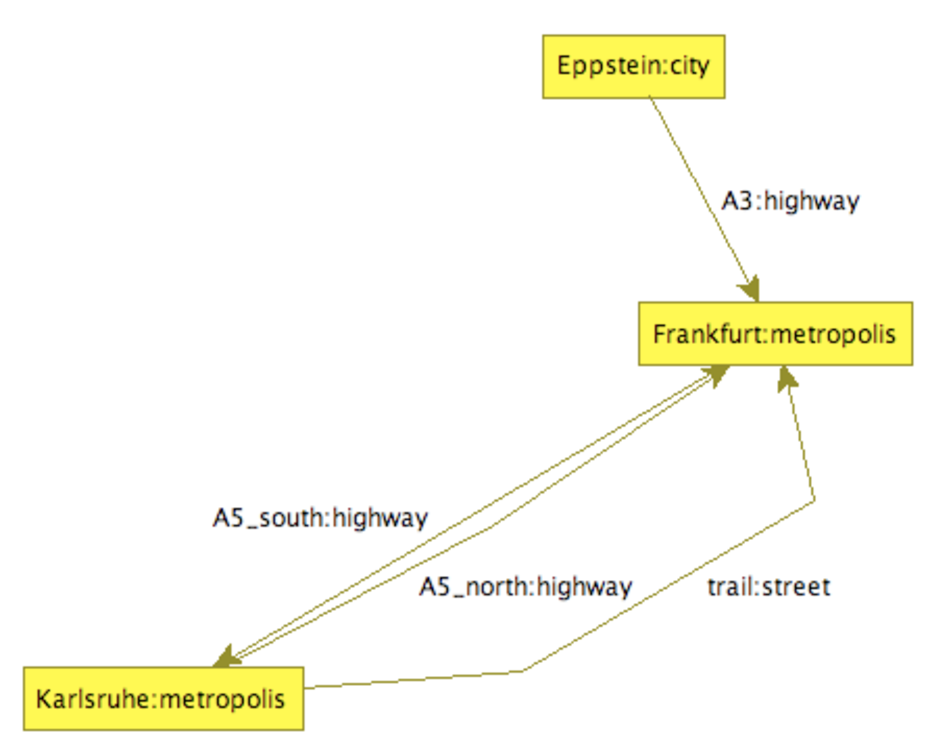
\includegraphics[width=8.5cm]{fig/map}}
\end{center}

This graph is valid but not strict valid.
\begin{grshell} 
> validate
The graph is valid.
> validate strict
The graph is NOT valid:
  CAE: city "Eppstein" -- highway "A3" --> metropolis "Frankfurt" not specified
  CAE: metropolis "Karlsruhe" -- street "trail" --> metropolis "Frankfurt" not specified
>
\end{grshell}
\end{example}

\begin{rail}
  'validate' ('exitonfailure')? 'xgrs' GRS
\end{rail}\ixkeyw{validate}\ixkeyw{grs}
Validates\indexmain{validate} if the current working graph satisfies the \indexed{graph rewrite sequence} given.
Before the graph rewrite sequence is executed, the instance graph gets cloned;
the sequence operates on the clone, allowing you to change the graph as you want to, without influence on the host graph.
Validation fails iff the xgrs fails.
This gives a rather costly but extremely flexible and powerful mechanism to specify graph constraints.
The GrShell is exited with an error code if \texttt{exitonfailure} is specified and the validation fails.


\subsection{Visited Flag Commands}

\begin{rail}
'Variable' '=' 'allocvisitflag'
\end{rail}\ixkeyw{allocvisitflag}\label{allocvisitflag}
Allocates space for a visited flag in the elements of the graph and returns the id of the visited flag (integer number), starting at 0.
Afterwards, the visited flag of the id can be read and written within the rules by the \texttt{visited}-expression and the \texttt{visited}-assignment,
as well as by the \texttt{isvisited} and \texttt{setvisited} shell commands.
The first visited flags are stored in some excess bytes of the graph elements and are thus essentially for free, but if this implementation defined space is used up completely, the information is stored in dictionaries.

\begin{rail}
'freevisitflag' 'Variable'
\end{rail}\ixkeyw{freevisitflag}
Frees the space previously allocated for the visited flag; afterwards you must not access it anymore. 
The value stored in the variable must be of integer type, stemming from a previous allocation.

\begin{rail} 
'setvisited' GraphElement 'flagId' 'BooleanValue'
\end{rail}\ixkeyw{setvisited}
Sets the visited status of the graph element of the flag id the given boolean value; visited flags are normally written by rules of the rule language.

\begin{rail}
'isvisited' GraphElement 'flagId'
\end{rail}\ixkeyw{isvisited}
Returns the visited status of the graph element of the flag id; visited flags are normally read by tests and rules of the rule language.


\subsection{Graph Input and Output Commands}
\label{outputcmds}

\begin{rail}
  'save' 'graph' Filename
\end{rail}\ixkeyw{save}\ixkeyw{graph}
Dumps\indexmain{dumping graph} the current graph as \GrShell\ script\indexmain{graph rewrite script} into \emph{Filename}.
The created script includes
\begin{itemize}
  \item selecting the backend
  \item creating a new graph with all nodes and edges (including their persistent names)
  \item restoring the variables
  \item restoring the visualisation styles
\end{itemize}
but not necessarily using the same commands you typed in during construction. 
Such a script can be loaded and executed by the \texttt{include} command (see Section~\ref{commcommands}).

\begin{rail}
  'export' Filename.grs (withvariables)?
\end{rail}\ixkeyw{export}
Exports an instance graph in GRS format, which is a reduced \GrShell\ script (it can get imported and exported on API level\ref{sub:imexport} without using the \GrShell\).
It contains the \texttt{new graph} command, followed by \texttt{new node} commands, followed by \texttt{new edge} commands.
If \texttt{withvariables} is specified, the variables are exported, too.
The export is only complete with the model of the graph given in the \texttt{.gm} file.
Exporting fails if the graph model contains attributes of \texttt{object}-type.
The \texttt{save} command is for saving a \GrShell\ session including visualization styles, the goal of the \texttt{export} command is graph rewrite system interoperability.

\begin{rail}
  'export' Filename.gxl
\end{rail}\ixkeyw{export}
Exports an instance graph and a graph model in GXL format \ref{}, which is somewhat of a standard format for graphs of graph rewrite systems, but suffers from the well-known XML problems -- it is barely human-readable and bloated.
Exporting fails if the graph model contains attributes of \texttt{set<S>}-,\texttt{map<S,T>}-, or \texttt{object}-type.

\begin{rail}
  'import' Filename.grs
\end{rail}\ixkeyw{import}
Imports the specified graph instance in GRS format (the \emph{reduced} \GrShell\ script, a saved graph can only be imported by \texttt{include} (but an exported graph can be imported by \texttt{include}, too)).
The referenced graph model must be available as \texttt{.gm}-file.

\begin{rail}
  'import' Filename.gxl (ModelOverride)?
\end{rail}\ixkeyw{import}
Imports the specified graph instance and model in GXL format.
If a model override of the form \texttt{Filename.gm} is specified, the given model will be used instead of the model in the GXL file.
The \texttt{.gxl}-graph must be compatible to the \texttt{.gm}-model.

\begin{note}
Normally you are not only interested in importing a GXL graph (and viewing it), but you want to execute actions on it.
The problem is that the actions are model dependent.
So, in order to apply actions, you must use a model override, which works this way:
\begin{enumerate}
\item \texttt{new graph "YourName.grg"}\\
This creates the model library lgsp-YourNameModel.dll
and the actions library lgsp-YourNameActions.dll
(which depends on the model library generated from the \texttt{"using YourName;"}).
\item \texttt{import InstanceGraphOnly.gxl YourName.gm}\\
This imports the instance graph from the .gxl but uses the model specified
in YourName.gm (it must fit to the model in the .gxl in order to work).
\item \texttt{select actions lgsp-YourNameActions.dll}\\
This loads the actions from the actions library in addition to the already
loaded model and instance graph (cf. \ref{grsthings}).
\item Now you are ready to use the actions.
\end{enumerate}
\end{note}


\subsection{Graph Manipulation Commands}
\label{mani}
Graph manipulation commands alter existing graphs; they allow to create and delete graph elements and change attributes. 
These are tasks which should be carried by the rules of the rule language -- the commands are mainly used as elementary instructions in graph input and output.

\begin{rail}
  'new' (() | Text) (() | ':' NodeType (() | Constructor))
\end{rail}\ixkeyw{new}
Creates a new node within the current graph.
Optionally a variable \emph{Text} is assigned to the new node.
If \emph{NodeType} is supplied, the new node will be of type \emph{NodeType} and attributes can be initialized by a constructor.
Otherwise the node will be of the base node class type \emph{Node}.
\begin{note}
The \GrShell\ can reassign \indexed{variable}s. 
This is in contrast to the rule language (chapter~\ref{chaprulelang}), where we use \emph{names}\indexmain{name}.
\end{note}

\begin{rail}
  'new' Node '-' (()|Text) \\ (() | ':' EdgeType (() | Constructor)) '->' Node
\end{rail}\ixkeyw{new}
Creates a new edge within the current graph between the specified nodes, directed towards the second \emph{Node}.
Optionally a variable \emph{Text} is assigned to the new edge.
If \emph{EdgeType} is supplied, the new edge will be of type \emph{EdgeType} and attributes can be initialized by a constructor.
Otherwise the edge will be of the base edge class type \emph{Edge}.

\begin{rail}
  Constructor : '(' (() | (dollar '=' Text (() | ',' Attributes) | Attributes)) ')';
  Attributes : AttributeName '=' (Text | Number) + ',' ;
\end{rail}\indexmain{\texttt{\$}}\ixnterm{Constructor}\ixnterm{Attributes}
A \indexed{constructor} is used to initialize a new graph element (see \texttt{new \dots} below).
A comma separated list of \indexed{attribute} declarations is supplied to the constructor.
Available attribute names are specified by the graph model of the current working graph.
All the undeclared attributes will be initialized with \indexed{default value}s, depending on their type (int $\leftarrow$ \texttt{0}, enum $\leftarrow$ unspecified; boolean $\leftarrow$ \texttt{false}; float, double $\leftarrow$ \texttt{0.0}; string $\leftarrow$ \texttt{""}).\\
The \texttt{\$} is a special attribute name: a unique identifier of the new graph element.
This identifier is also called \newterm{persistent name} (see Example~\ref{persistentex}).
This name can be specified by a constructor only.
TODO: set/map constructor

\begin{rail}
  'delete' 'node' Node
\end{rail}\ixkeyw{delete}\ixkeyw{node}
Deletes the node \emph{Node} from the current graph.
Incident edges will be deleted as well.

\begin{rail}
  'delete' 'edge' Edge
\end{rail}\ixkeyw{delete}\ixkeyw{edge}
Deletes the edge \emph{Edge} from the current graph.

\begin{rail}
  GraphElement '.' AttributeName '=' (Text | Number) ;
\end{rail}
Set the \indexed{attribute} \emph{AttributeName} of the graph element \emph{GraphElement} to the value of \emph{Text} or \emph{Number}.

  
\subsection{Graph and Model Query Commands}

todo: n.a, e.a shows the content of the attribute
todo: change this to show n.a, show e.a for consistency?

\begin{rail}
  'show' (() | 'num') ('nodes' (() | (() | 'only') NodeType) | 'edges' (() | (() | 'only') EdgeType))
\end{rail}\ixkeyw{show}\ixkeyw{num}\ixkeyw{nodes}\ixkeyw{edges}\ixkeyw{only}
Gets the \indexed{persistent name}s and the types of all the nodes/edges of the current graph. 
If a node type or edge type is supplied, only elements compatible to this type are considered. 
The \texttt{only} keyword excludes subtypes. Nodes/edges without persistent names are shown with a pseudo-name.
If the command is specified with \texttt{num}, only the number of nodes/edges will be displayed.

\begin{rail}
  'show' ('node' | 'edge') 'types'
\end{rail}\ixkeyw{show}\ixkeyw{node}\ixkeyw{edge}
Gets the node/edge types of the current graph model.

\begin{rail}
'show' ('node' ('super' | 'sub') 'types' NodeType | 'edge' ('super' | 'sub') 'types' EdgeType)
\end{rail}\ixkeyw{show}\ixkeyw{node}\ixkeyw{edge}\ixkeyw{super}\ixkeyw{sub}\indexmain{inheritance}
Gets the inherited/descendant types of \emph{NodeType}/\emph{EdgeType}.

\begin{rail}
  'show' ('node' 'attributes' (() | (() | 'only') NodeType) | 'edge' 'attributes' (() | (() | 'only') EdgeType))
\end{rail}\ixkeyw{show}\ixkeyw{node}\ixkeyw{edge}\ixkeyw{only}
Gets the available node/edge \indexed{attribute} types.
If \emph{NodeType}/\emph{EdgeType} is supplied, only attributes defined in \emph{NodeType}/\emph{EdgeType} are diplayed.
The \texttt{only} keyword excludes inherited attributes.\\
\begin{note}
The \texttt{show nodes/edges attributes\dots} command covers types and \emph{inherited} types.
This is in contrast to the other \texttt{show\dots} commands where types and \emph{sub}types are specified or the direction in the type hierarchy is specified explicitly, respectively.
\end{note}

\begin{rail}
 'show' ('node' Node | 'edge' Edge)
\end{rail}\ixkeyw{show}\ixkeyw{node}\ixkeyw{edge}
Gets the attribute types and values of a specific graph element.

\begin{rail}
 'show' 'var' Var
\end{rail}\ixkeyw{show}\ixkeyw{variable}
Displays the type and value of the specified variable.

\begin{rail}
  'show' GraphElement '.' AttributeName
\end{rail}\ixkeyw{show}\ixkeyw{attribute}
Displays the value of the specified attribute.

\begin{rail}
  'node' 'type' Node 'is' Node | 'edge' 'type' Edge 'is' Edge
\end{rail}\ixkeyw{node}\ixkeyw{edge}\ixkeyw{type}\ixkeyw{is}
Gets the information whether the first element is \indexed{type-compatible}\indexmainsee{compatible types}{type-compatible} to the second element.


\subsection{Graph Visualization Commands}

\begin{rail}
  'show' 'graph' ExecutableName (() | Text)
\end{rail}\ixkeyw{show}\ixkeyw{graph}
Dumps the current graph in \indexed{VCG} format into a temporary file.
The temporary VCG file will be passed to the program \emph{ExecutableName} as first parameter;
further parameters, such as program options, can be specified by \emph{Text}.
If you use \yComp\footnote{See Section~\ref{tools:ycomp}.}\indexmain{yComp} as executable (\texttt{show graph ycomp}), this may look like
\begin{center}
  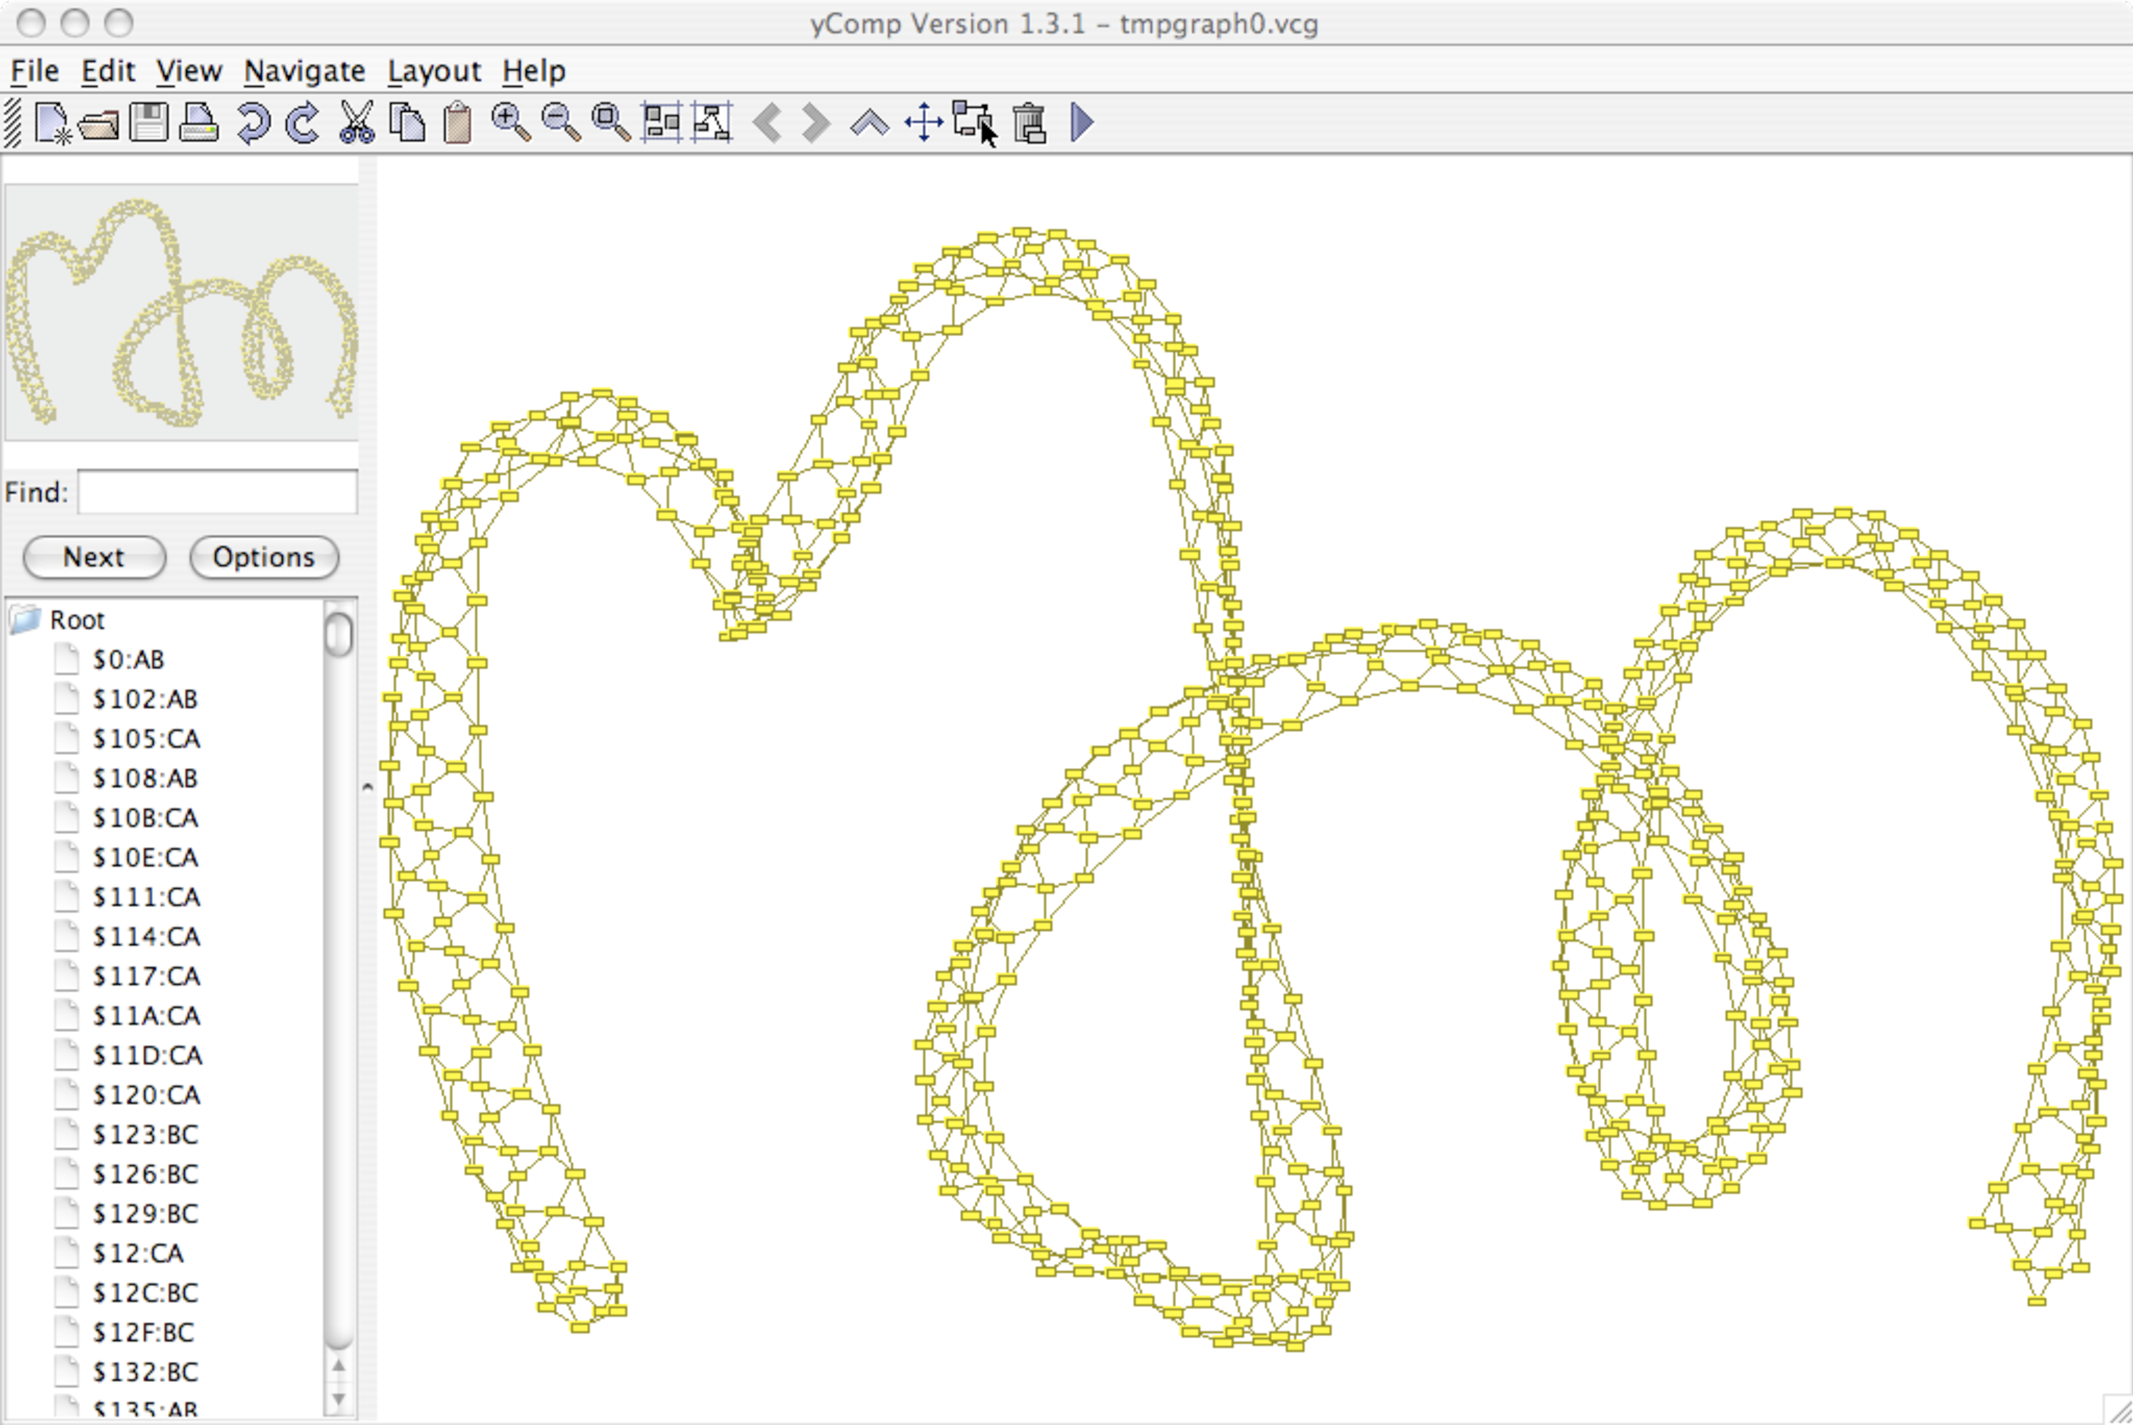
\includegraphics[width=0.75\linewidth]{fig/showgraph}
\end{center}  
The temporary file will be deleted, when the application \emph{Filename} is terminated if \GrShell\ is still running at this time.

\begin{rail}
  'dump' 'graph' Filename
\end{rail}\ixkeyw{dump}\ixkeyw{graph}
Dumps the current graph in \indexed{VCG} format into the file \emph{Filename}.\\

The following commands control the style of the VCG output. This affects \texttt{dump graph}, \texttt{show graph}, and \texttt{enable debug}. 
\begin{rail}
  'dump' 'set' 'node' (() | 'only') NodeType \\ (('color' | 'textcolor' | 'bordercolor') Color | 'shape' Text | 'labels' ('on' | 'off' | Text)) ;
\end{rail}\ixkeyw{dump}\ixkeyw{set}\ixkeyw{node}\ixkeyw{only}\ixkeyw{color}\ixkeyw{textcolor}\ixkeyw{bordercolor}\ixkeyw{shape}\ixkeyw{labels}
Sets the \indexed{color}, text color, border color, the shape or the label of the nodes of type \emph{NodeType} and all of its subtypes.
The keyword \texttt{only} excludes the subtypes. The available colors are specified at the begin of this chapter. 
The following shapes are supported: \texttt{box}, \texttt{triangle}, \texttt{circle}, \texttt{ellipse}, \texttt{rhom}, \texttt{hexagon}, \texttt{trapeze}, \texttt{uptrapeze}, \texttt{lparallelogram}, \texttt{rparallelogram}.
Those are shape names of \yComp\ (for a VCG definition see~\cite{vcg}).
The default labeling is set to \texttt{on} with \texttt{Name:Type}, it can be overwritten by an specified label string (e.g. the source code line originating the node in a program graph) or switched off.

\begin{rail}
  'dump' 'set' 'edge' (() | 'only') EdgeType \\ (('color' | 'textcolor') Color | 'labels' ('on' | 'off' | Text));
\end{rail}\ixkeyw{dump}\ixkeyw{set}\ixkeyw{edge}\ixkeyw{only}\ixkeyw{color}\ixkeyw{textcolor}\ixkeyw{labels}
Sets the color, text color or label of the edges of type \emph{EdgeType} and all of its subtypes.
The keyword \texttt{only} excludes the subtypes. The available colors are specified at the begin of this chapter.
The default labeling is set to \texttt{on} with \texttt{Name:Type}, it can be overwritten by an specified label string or switched off.

\begin{rail}
  'dump' 'add' 'node' ('only')? NodeType 'exclude' ;
\end{rail}\ixkeyw{dump}\ixkeyw{add}\ixkeyw{node}\ixkeyw{only}\ixkeyw{exclude}
Excludes nodes of type \emph{NodeType} and all of its subtypes as well as their incident edges from output.
The keyword \texttt{only} excludes the subtypes from exlusion, i.e.\ subtypes of \emph{NodeType} are dumped.

\begin{rail}
  'dump' 'add' 'node' ('only')? NodeType 'group' (GroupConstraints)? ;
GroupConstraints:
  'by' ('hidden')? GroupMode (IncAdjTypeConstraints)? ;
IncAdjTypeConstraints:
  ('only')? EdgeType ('with' ('only')? NodeType)? ;
\end{rail}\ixkeyw{dump}\ixkeyw{add}\ixkeyw{node}\ixkeyw{group}
Declares \emph{NodeType} and subtypes of \emph{NodeType} as \indexed{group node} type.
All the differently typed nodes that point to a node of type \emph{NodeType} 
(i.e.\ there is a directed edge between such nodes) will be grouped and visibly enclosed by the \emph{NodeType}-node.
\texttt{GroupMode} is one of \texttt{no},\texttt{incoming},\texttt{outgoing},\texttt{any}; \texttt{hidden} causes hiding of the edges by which grouping happens.
The \texttt{EdgeType} constrains the type of the edges which cause grouping, the \texttt{with} clause additionally constains the type of the adjacent node; 
\texttt{only} excludes subtypes.

The following example shows \emph{metropolis} ungrouped and grouped:
\begin{center}
  \fbox{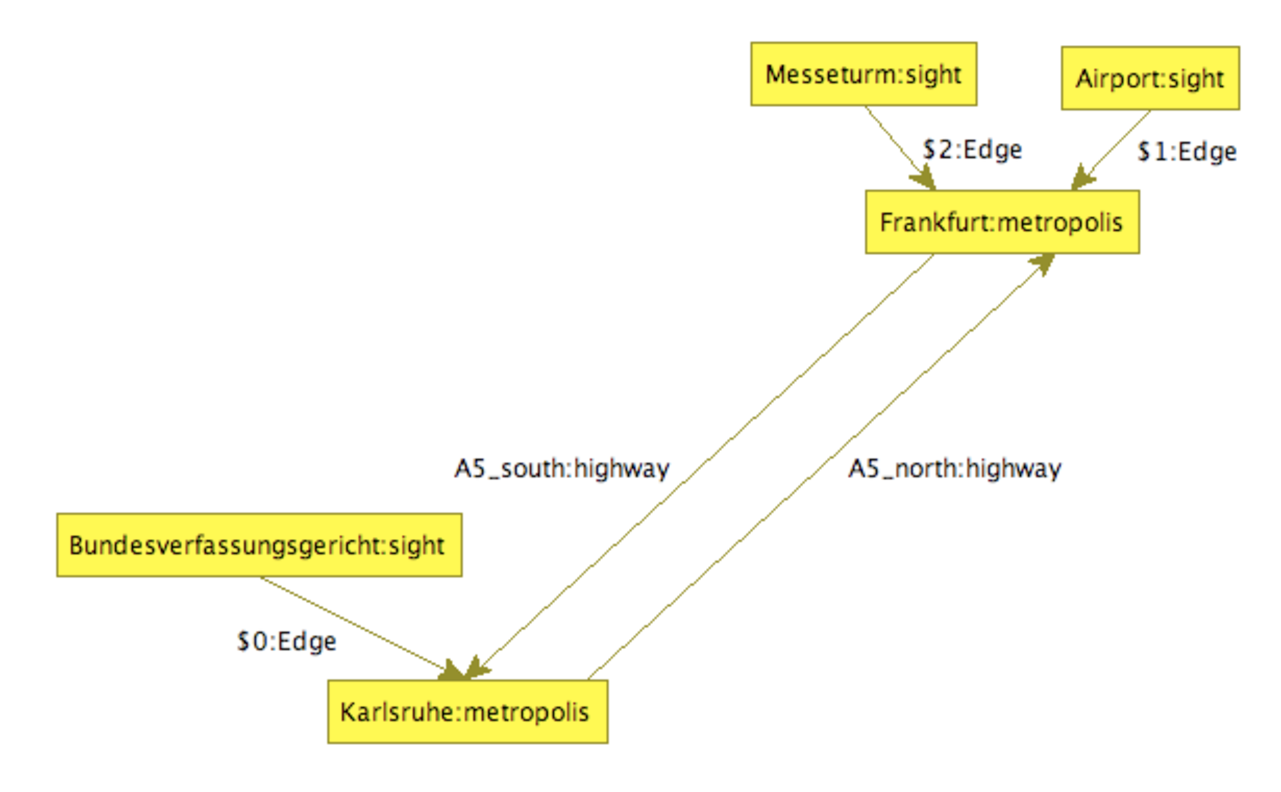
\includegraphics[width=0.45\linewidth]{fig/group2-1}}  \hfill \fbox{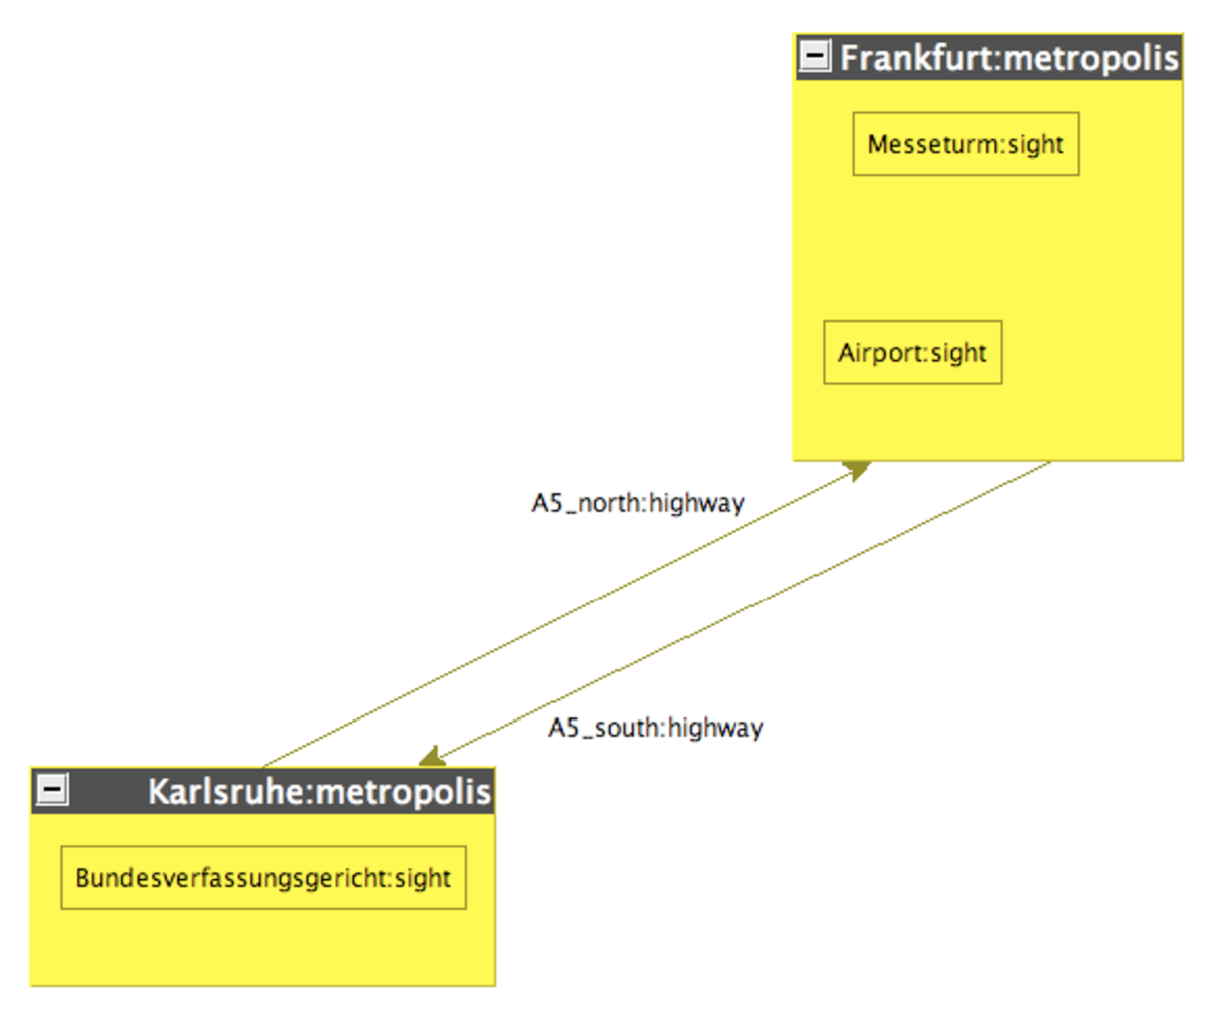
\includegraphics[width=0.45\linewidth]{fig/group2-2}}\\
  {\small right side: dumped with \texttt{dump add node metropolis group}}
\end{center}

\begin{rail}
  'dump' 'add' (() | 'only') ('node' NodeType | 'edge' EdgeType) \\ ('infotag' | 'shortinfotag') AttributeName
\end{rail}\ixkeyw{dump}\ixkeyw{add}\ixkeyw{only}\ixkeyw{node}\ixkeyw{edge}\ixkeyw{infotag}
Declares the \indexed{attribute} \emph{AttributeName} to be an ``\indexed{info tag}'' or ``\indexed{short info tag}''.
Info tags are displayed like additional node/edge \indexed{label}s, in format \texttt{Name=Value}, or \texttt{Value} only for short info tags. 
The keyword \texttt{only} excludes the subtypes of \emph{NodeType} resp.\ \emph{EdgeType}. 
In the following example \emph{river} and \emph{jam} are info tags:
\begin{center}
  \fbox{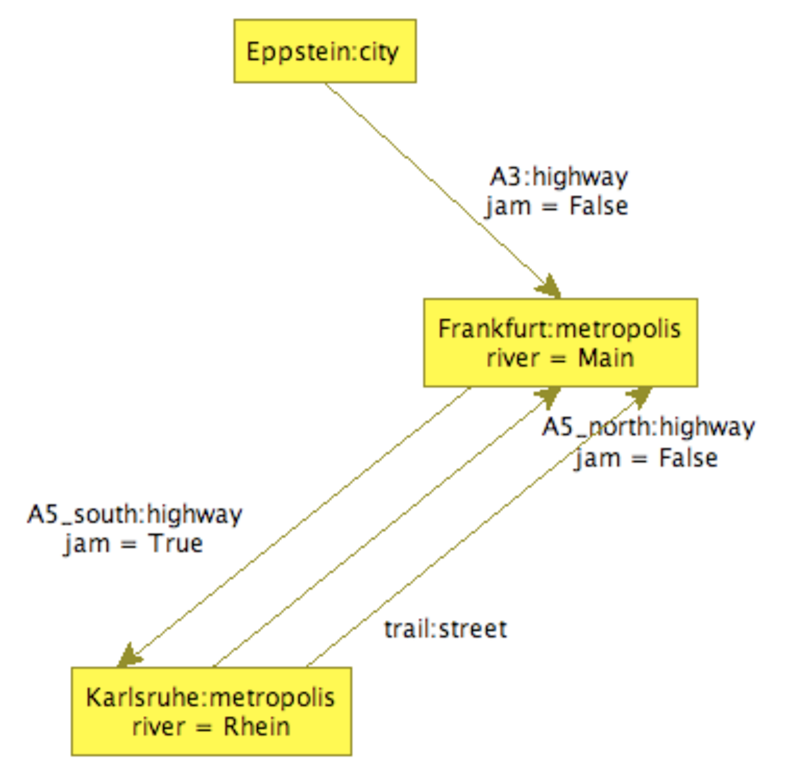
\includegraphics[width=0.5\linewidth]{fig/infotag}}
\end{center}

\begin{rail}
  'dump' 'reset'
\end{rail}\ixkeyw{dump}\ixkeyw{reset}
Resets all style options (\texttt{dump set}\dots) to their default values.


\begin{note}
Small graphs allow for fast visual understanding, but with an increasing number of nodes and edges they quickly loose this property.
The group commands are of outstanding importance to keep readability with increasing graph sizes
(e.g. for program graphs it allows to lump together expressions of a method inside the method node and attributes of the class inside the class node).
Additional helpers in keeping the graph readable are: 
the capability to exclude elements from dumping (the less hay in the stack the easier to find the needle),
the different colors and shapes to quickly find the elements of interest,
as well as the labels/infotags/shortinfotags to display the most important information directly. 
Choose the layout algorithm and the options delivering the best results for your needs, organic and compiler graph 
(an extension of hierarchic with automatic edge cutting -- marking cut edges by fat dots, showing the edge only on mouse over and allowing to jump to the other end on a mouse click)
should be tried first.
\end{note}


\subsection{Action Commands (XGRS)}\indexmain{action command}\indexmainsee{action}{graph rewrite sequence}
\label{grsthings}
An \emph{action} denotes a graph rewrite rule.

\begin{rail}
  'select' 'actions' Filename
\end{rail}\ixkeyw{select}\ixkeyw{actions}
Selects a \indexed{rule set}.
\emph{Filename} can either be a .NET assembly (e.g.\ ``rules.dll'') or a source file (``rules.cs'').
Only one rule set can be loaded simultaneously.

\begin{rail}
  'show' 'actions'
\end{rail}\ixkeyw{show}\ixkeyw{actions}
Lists all the rules of the loaded rule set, their parameters, and their return values.
Rules can return a set of graph elements.

\begin{rail}
  'custom' 'actions' (() | SpacedParameters)
\end{rail}\ixkeyw{custom}\ixkeyw{actions}
Executes an action specific to the current \indexed{backend}. 
If \emph{SpacedParameters} is omitted, a list of available commands will be displayed (for the LGSPBackend see Section~\ref{custom}).

\makeatletter
\begin{rail}
  GraphRewriteSequence: 'xgrs' SimpleRewriteSequence ;
\end{rail}\ixkeyw{grs}\indexmain{graph rewrite sequence}\indexmainsee{GRS}{graph rewrite sequence}\ixnterm{GraphRewriteSequence}
This executes the graph rewrite sequence \emph{SimpleRewriteSequence}.
See section \ref{sct:xgrs} for graph rewrite sequences.
Additionally to the variable assignment in rule-embedded graph rewrite sequences, you are also able to assign \emph{persistent names} to parameters via  \texttt{Variable = \@(Text)}.

Graph elements returned by rules can be assigned to variables\indexmain{variable} using \texttt{(Para\-meters) = \emph{Action}}\indexmain{parameter}. 
The desired variable identifiers have to be listed in \emph{Parameters}. 
Graph elements required by rules must be provided using \texttt{Action (Para\-meters)}, where \emph{Parameters} is a list of variable identifiers. 
For \indexed{undefined variables} see Section~\ref{ruledecls}, \emph{Parameters}.

% don't explain set/map commands, as they will be replaced by graph rewrite sequence terms
% they are given in the changelog, so if someone needs them now they are there
% but not fully officially documented, so that they can be dropped as soon as the sequences are extended


\section{Graphical Debugger}
\label{sct:debugger}
The \GrShell\ together with \yComp\ build \GrG's graphical debugger.

\subsection{Debugging Related Commands}

\begin{rail}
  'debug' ( 'enable' | 'disable' )
\end{rail}\ixkeyw{debug}\ixkeyw{enable}\ixkeyw{disable}
Enables and disables the \indexed{debug mode}.
The debug mode shows the current working graph in a \yComp\ window.
All changes to the working graph are tracked by \yComp\ immediately.  

\begin{rail}
  'debug' 'set' 'layout' ( (Text)? | 'option' Name String ) ;
\end{rail}\ixkeyw{debug}\ixkeyw{set}\ixkeyw{layout}
Sets the default graph \indexed{layout algorithm} to \emph{Text}.
If \emph{Text} is omitted, a list of available layout algorithms is displayed.
See Section~\ref{tools:ycomp} on \yComp\ layouters.
The \texttt{option} version allows to specify layout options by name value pairs.
The available layout options can be listed by the following command.

\begin{rail}
  'debug' 'get' 'layout' 'options';
\end{rail}\ixkeyw{debug}\ixkeyw{layout}
Prints a list of the available layout options of the layout algorithm.

\begin{rail}
  'debug' 'layout';
\end{rail}\ixkeyw{debug}\ixkeyw{layout}
Forces re-layout of the graph shown in yComp (same as pressing the play button within yComp).

\begin{rail}
  GraphRewriteSequence: 'debug' 'xgrs' SimpleRewriteSequence ;
\end{rail}\ixkeyw{debug}\ixkeyw{grs}\indexmain{graph rewrite sequence}\indexmainsee{GRS}{graph rewrite sequence}\ixnterm{GraphRewriteSequence}
This executes the graph rewrite sequence \emph{SimpleRewriteSequence} in the debugger\indexmain{debugger}.
Same as \texttt{xgrs SimpleRewriteSequence} in the previous section, but allows tracing the rewriting process step-by-step. 

\begin{rail}
'debug' 'apply' Rule
\end{rail}\ixkeyw{debug}\ixkeyw{apply}
The \texttt{debug apply} command allows to interactively select parameters for the execution of the rule \texttt{Rule}.
The parameters to select are specified by the wildcard elements \texttt{?}, they are given by double clicking at elements in the graph viewer yComp.

\begin{example}
\begin{grshelllet}
debug apply r(?, x, ?)
\end{grshelllet}
will prompt the user for input of the first and the third parameter, while the second one is taken from variable x.
\end{example}


\subsection{Using the Debugger}

During execution \yComp\footnote{Make sure, that the path to your \texttt{\indexed{yComp.jar}} package is set correctly in the \texttt{ycomp} shell script within \GrG's \texttt{/bin} directory.}
\indexmain{yComp} will display every single step. 
The debugger\indexmain{debugger} can be controlled by \GrShell. 
Remember that the \texttt{\%} modifier before a rule works as break point in a graph rewrite sequence.
The debug commands are shown in Table~\ref{tabdebug}. A run is shown in the following example \ref{ex:debug}.
\begin{table}[htbp]
  \begin{tabularx}{\linewidth}{|lX|} \hline
  \texttt{s}(tep) & Execute the next rewrite rule (match and rewrite)\\
  \texttt{d}(etailed step) & Execute a rewrite rule in a three-step procedure: matching, highlighting elements to be changed, doing rewriting \\
  \texttt{n}(ext) & Ascend one level up within the \indexed{Kantorowitsch tree} of the current rewrite sequence (see Example~\ref{ex:debug})\\
  (step) \texttt{o}(ut) & Continue execution until the end of the current loop. If the execution is not in a loop at this moment, the complete sequence will be executed\\
  (toggle) \texttt{b}(reakpoint) & Toggle a breakpoint at a rewrite rule, a true, or a false\\
  \texttt{r}(un) & Continue execution\\
  \texttt{a}(bort) & Cancel the execution immediately\\ \hline 
  \end{tabularx}
  \caption{\GrShell\ debug commands}
  \label{tabdebug}
\end{table}
%\begin{figure}[htbp]
%  \centering
%  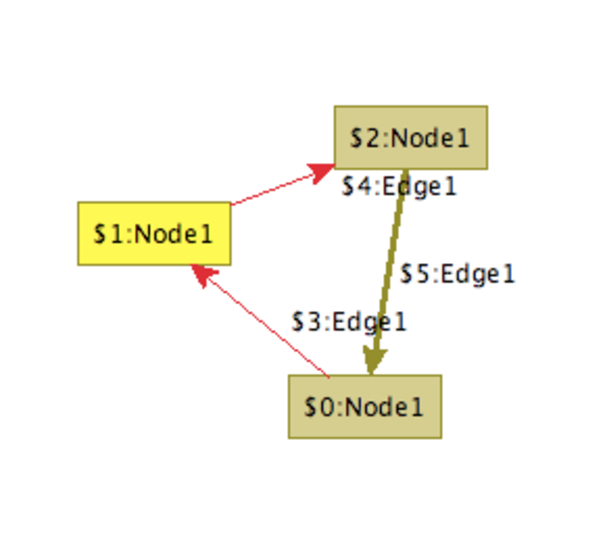
\includegraphics[width=0.25\linewidth]{fig/debug1}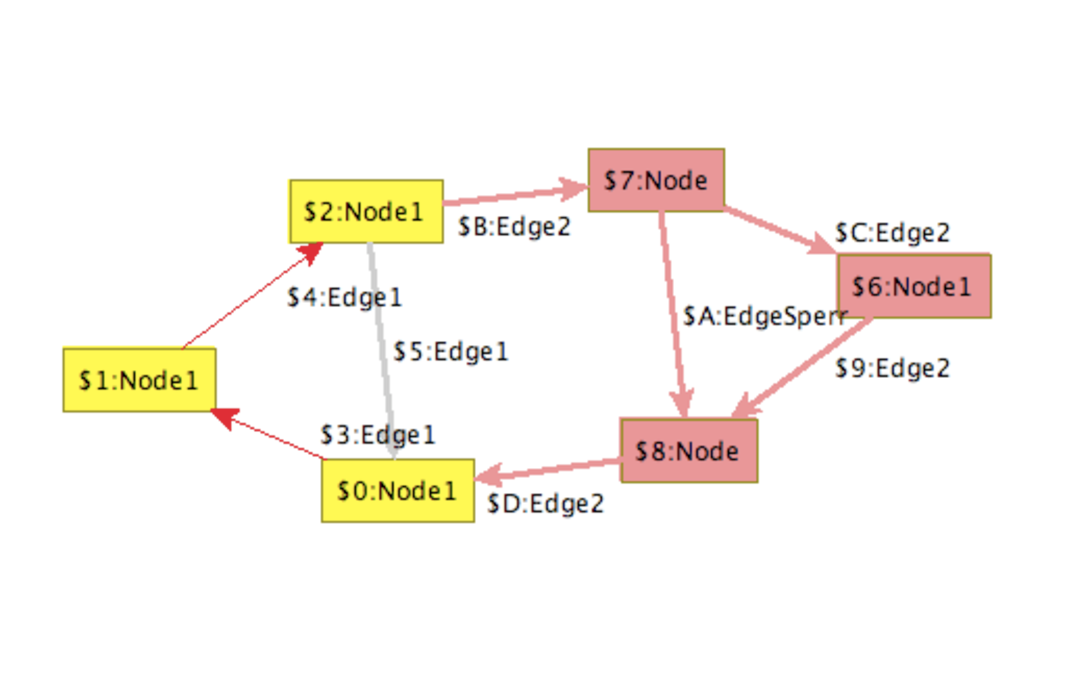
\includegraphics[width=0.4\linewidth]{fig/debug2}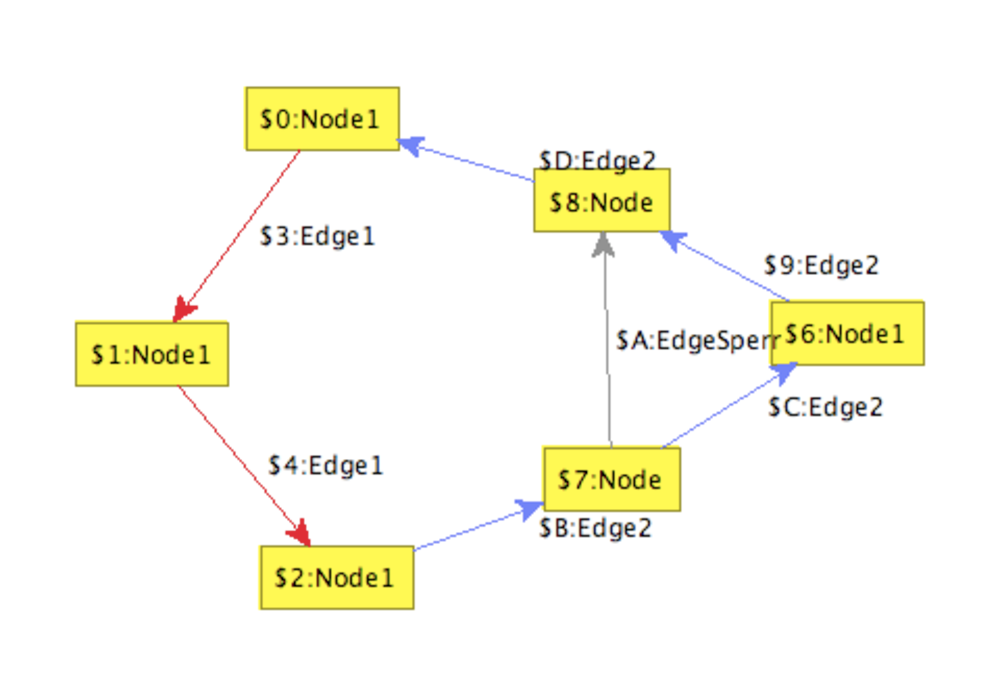
\includegraphics[width=0.4\linewidth]{fig/debug3}
%  \caption{Delayed step rule application.}
%  \label{figdebug}
%\end{figure}

\begin{figure}[htbp]
\begin{example}\label{ex:debug}  
We demonstrate the debug commands with a slightly adjusted script for the Koch snowflake from \GrG's examples (see also Section~\ref{fractals}). The graph rewriting sequence is
\begin{grshell}
debug xgrs (makeFlake1* & (beautify & doNothing)* & makeFlake2* & beautify*)[1]
\end{grshell}
\yComp\ will be opened with an initial graph (resulting from \texttt{grs init}):
\begin{center}
  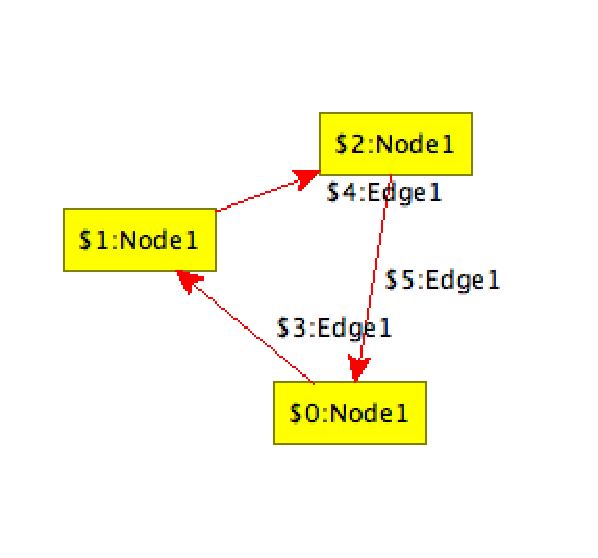
\includegraphics[width=0.3\linewidth]{fig/debug0tra}
\end{center}
We type \texttt{d}(etailed step) to apply \texttt{makeFlake1} step by step resulting in the following graphs:
\begin{center}
  \parbox{0.2\linewidth}{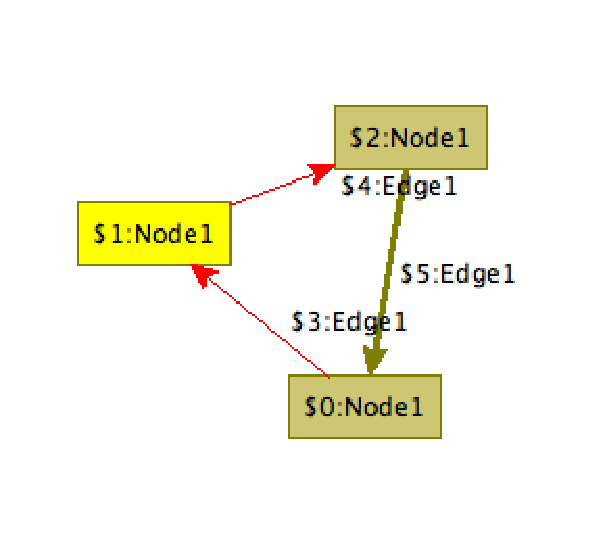
\includegraphics[width=\linewidth]{fig/debug1tra}}\parbox{0.375\linewidth}{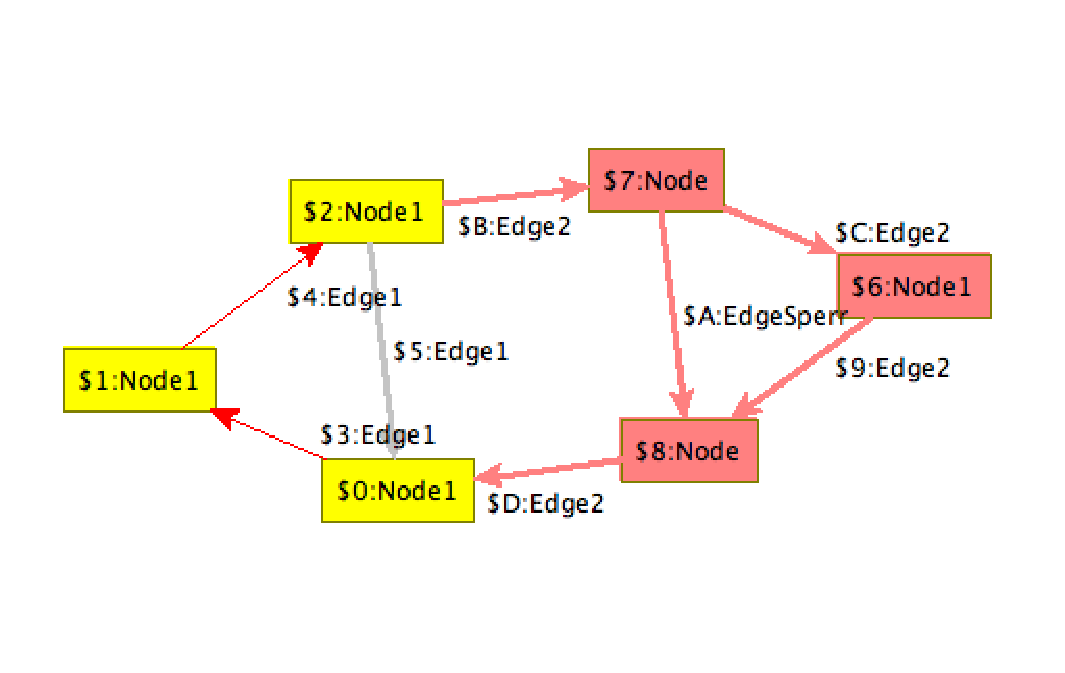
\includegraphics[width=\linewidth]{fig/debug2tra}}\parbox{0.375\linewidth}{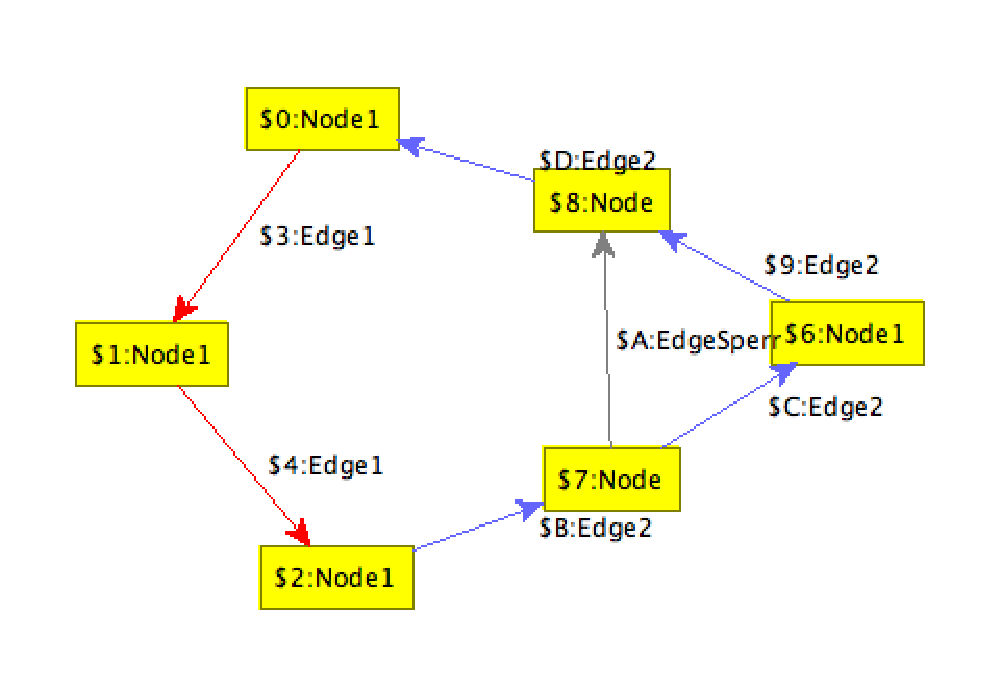
\includegraphics[width=\linewidth]{fig/debug3tra}}
\end{center}
The following table shows the ``break points'' of further debug commands, entered one after another:
\begin{center}
  \begin{tabular}{|l|l|} \hline
    \textbf{Command} & \textbf{Active rule} \\ \hline
    \texttt{s} & \texttt{makeFlake1} \\
    \texttt{o} & \texttt{beautify} \\
    \texttt{s} & \texttt{doNothing} \\
    \texttt{s} & \texttt{beautify} \\ 
    \texttt{n} & \texttt{beautify} \\ 
    \texttt{o} & \texttt{makeFlake2} \\
    \texttt{r} & --- \\ \hline
  \end{tabular}
\end{center}
\end{example}   
\end{figure}


\section{Backend Commands}
\label{backend}

\GrG\ is built to support multiple backends implementing the model and action interfaces of libGr.
This is roughly comparable to the different storage engines MySQL offers.
Currently only one backend is available, the libGr search plan backend, or short LGSPBackend.

\subsection{Backend selection and custom commands}

\begin{rail}
  'select' 'backend' Filename ( ( ) | ':' Parameters )
\end{rail}\ixkeyw{select}\ixkeyw{backend}
Selects a \indexed{backend} that handles graph and rule representation.
\emph{Filename} has to be a .NET assembly (e.g.\ \texttt{lgspBackend.dll}\indexmain{LGSPBackend}).
Comma-separated \indexed{parameter}s can be supplied optionally; if so, the backend must support these parameters.
By default the LGSPBackend is used.

\begin{rail}
  'show' 'backend'
\end{rail}\nopagebreak\ixkeyw{show}\ixkeyw{backend}
List all the parameters supported by the currently selected backend.
The parameters can be provided to the \texttt{select backend} command.

\begin{rail}
  'custom' 'graph' ( ( ) | SpacedParameters )
\end{rail}\ixkeyw{custom}\ixkeyw{graph}
Executes a command specific to the current backend.
If \emph{SpacedParameters} is omitted, a list of available commands will be displayed (for the LGSP backend see Sections~\ref{custom}).


\subsection{LGSPBackend Custom Commands}
\label{custom}

The \indexed{LGSPBackend} supports the following custom commands:

\begin{rail}
  'custom' 'graph' analyzegraph
\end{rail}\ixkeyw{custom}\ixkeyw{graph}
Analyzes\indexmain{analyzing graph} the current working graph.
The analysis data provides vital information for efficient \indexed{search plan}s.
Analysis data is available as long as \GrShell\ is running, i.e.\ when the working graph changes, the analysis data is still available but maybe obsolete.

\begin{rail}
  'custom' 'actions' gensearchplan (Action+)
\end{rail}\ixkeyw{custom}\ixkeyw{actions}
Creates a search plan for each rewrite rule \emph{Action} using a heuristic method and the analyzes data (if the graph has been analyzed by \texttt{custom graph analyze\_graph}).
Otherwise a \indexed{default search plan} is used.
For efficiency reasons it is recommended to do analyzing and search plan creation during the rewriting procedure.
Therefore the host graph should be in a stage ``similar'' to the final result.
Indeed there might be some trial-and-error steps necessary to get an efficient search plan.
A search plan is available as long as the current rule set remains loaded. 
Specify multiple rewrite rules instead of using multiple commands for each rule to improve the search plan generation performance.

\begin{rail}
  'custom' 'actions' setmaxmatches Number
\end{rail}\ixkeyw{custom}\ixkeyw{actions}
Sets the maximum amount of possible pattern matches to \emph{Number}.
This command affects the expression \texttt{[\emph{Rule}]}.
If \emph{Number} is less or equal to zero, the constraint is reset.



\chapter{Examples}
\label{anexample}

%%%%%%%%%%%%%%%%%%%%%%%%%%%%%%%%%%%%%%%%%%%%%%%%%%%%%%%%%%%%%%%%%%%%%%%%%%%%%%%%%%%%%%%%%%%%%%%%
\section{Fractals}\indexmain{example}
\label{fractals}
The \GrG\ package ships with samples for fractal generation. We will construct the \indexed{Sierpinski triangle} and the \indexed{Koch snowflake}. They are created by consecutive rule applications starting with the initial host graphs
\begin{center}
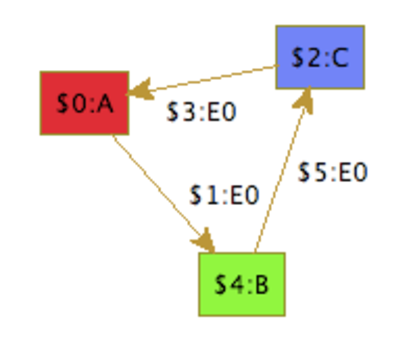
\includegraphics[width=4cm]{fig/startsir}\quad\quad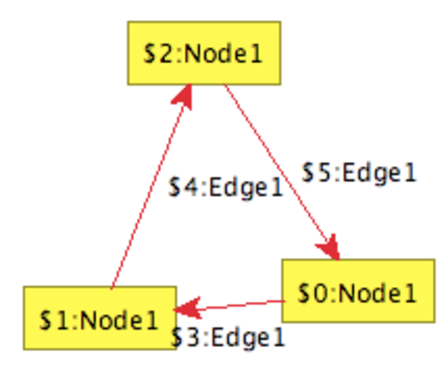
\includegraphics[width=4cm]{fig/startkoch}
\end{center}
for the Sierpinski triangle resp.\ the Koch snowflake.
First of all we have to compile the model and rule set files. So execute in \GrG's \texttt{bin} directory
\begin{verbatim}
GrGen.exe ..\specs\sierpinski.grg
GrGen.exe ..\specs\snowflake.grg
\end{verbatim}
or
\begin{verbatim}
mono GrGen.exe ../specs/sierpinski.grg
mono GrGen.exe ../specs/snowflake.grg
\end{verbatim}
respectively. If you are on a Unix-like system you have to adjust the path separators of the \GrShell\ scripts. Just edit the first three lines of \texttt{/test/Sierpinski.grs} and \texttt{/test/Snowflake.grs}. And as we have the file \texttt{Sierpinski.grs} already opened, we can increase the number of iterations to get even more beautiful graphs\footnote{Be careful: The running time increases exponentially in the number of iterations.}. Just follow the comments. Be careful when increasing the number of iterations of Koch's snowflake---\yComp's \indexed{layout algorithm} might need some time and attempts to layout it nicely.
We execute the Sierpinski script by
\begin{verbatim}
GrShell.exe ..\test\Sierpinski.grs
\end{verbatim}
or
\begin{verbatim}
mono GrShell.exe ../test/Sierpinski.grs
\end{verbatim}
respectively. Because both of the scripts are using the debug mode, we complete execution by typing \texttt{r}(un). See Section~\ref{grsthings} for further information. The resulting graphs should look like Figures~\ref{figsierp} and~\ref{figsnowflake}.
\begin{figure}[htbp]
  \centering
  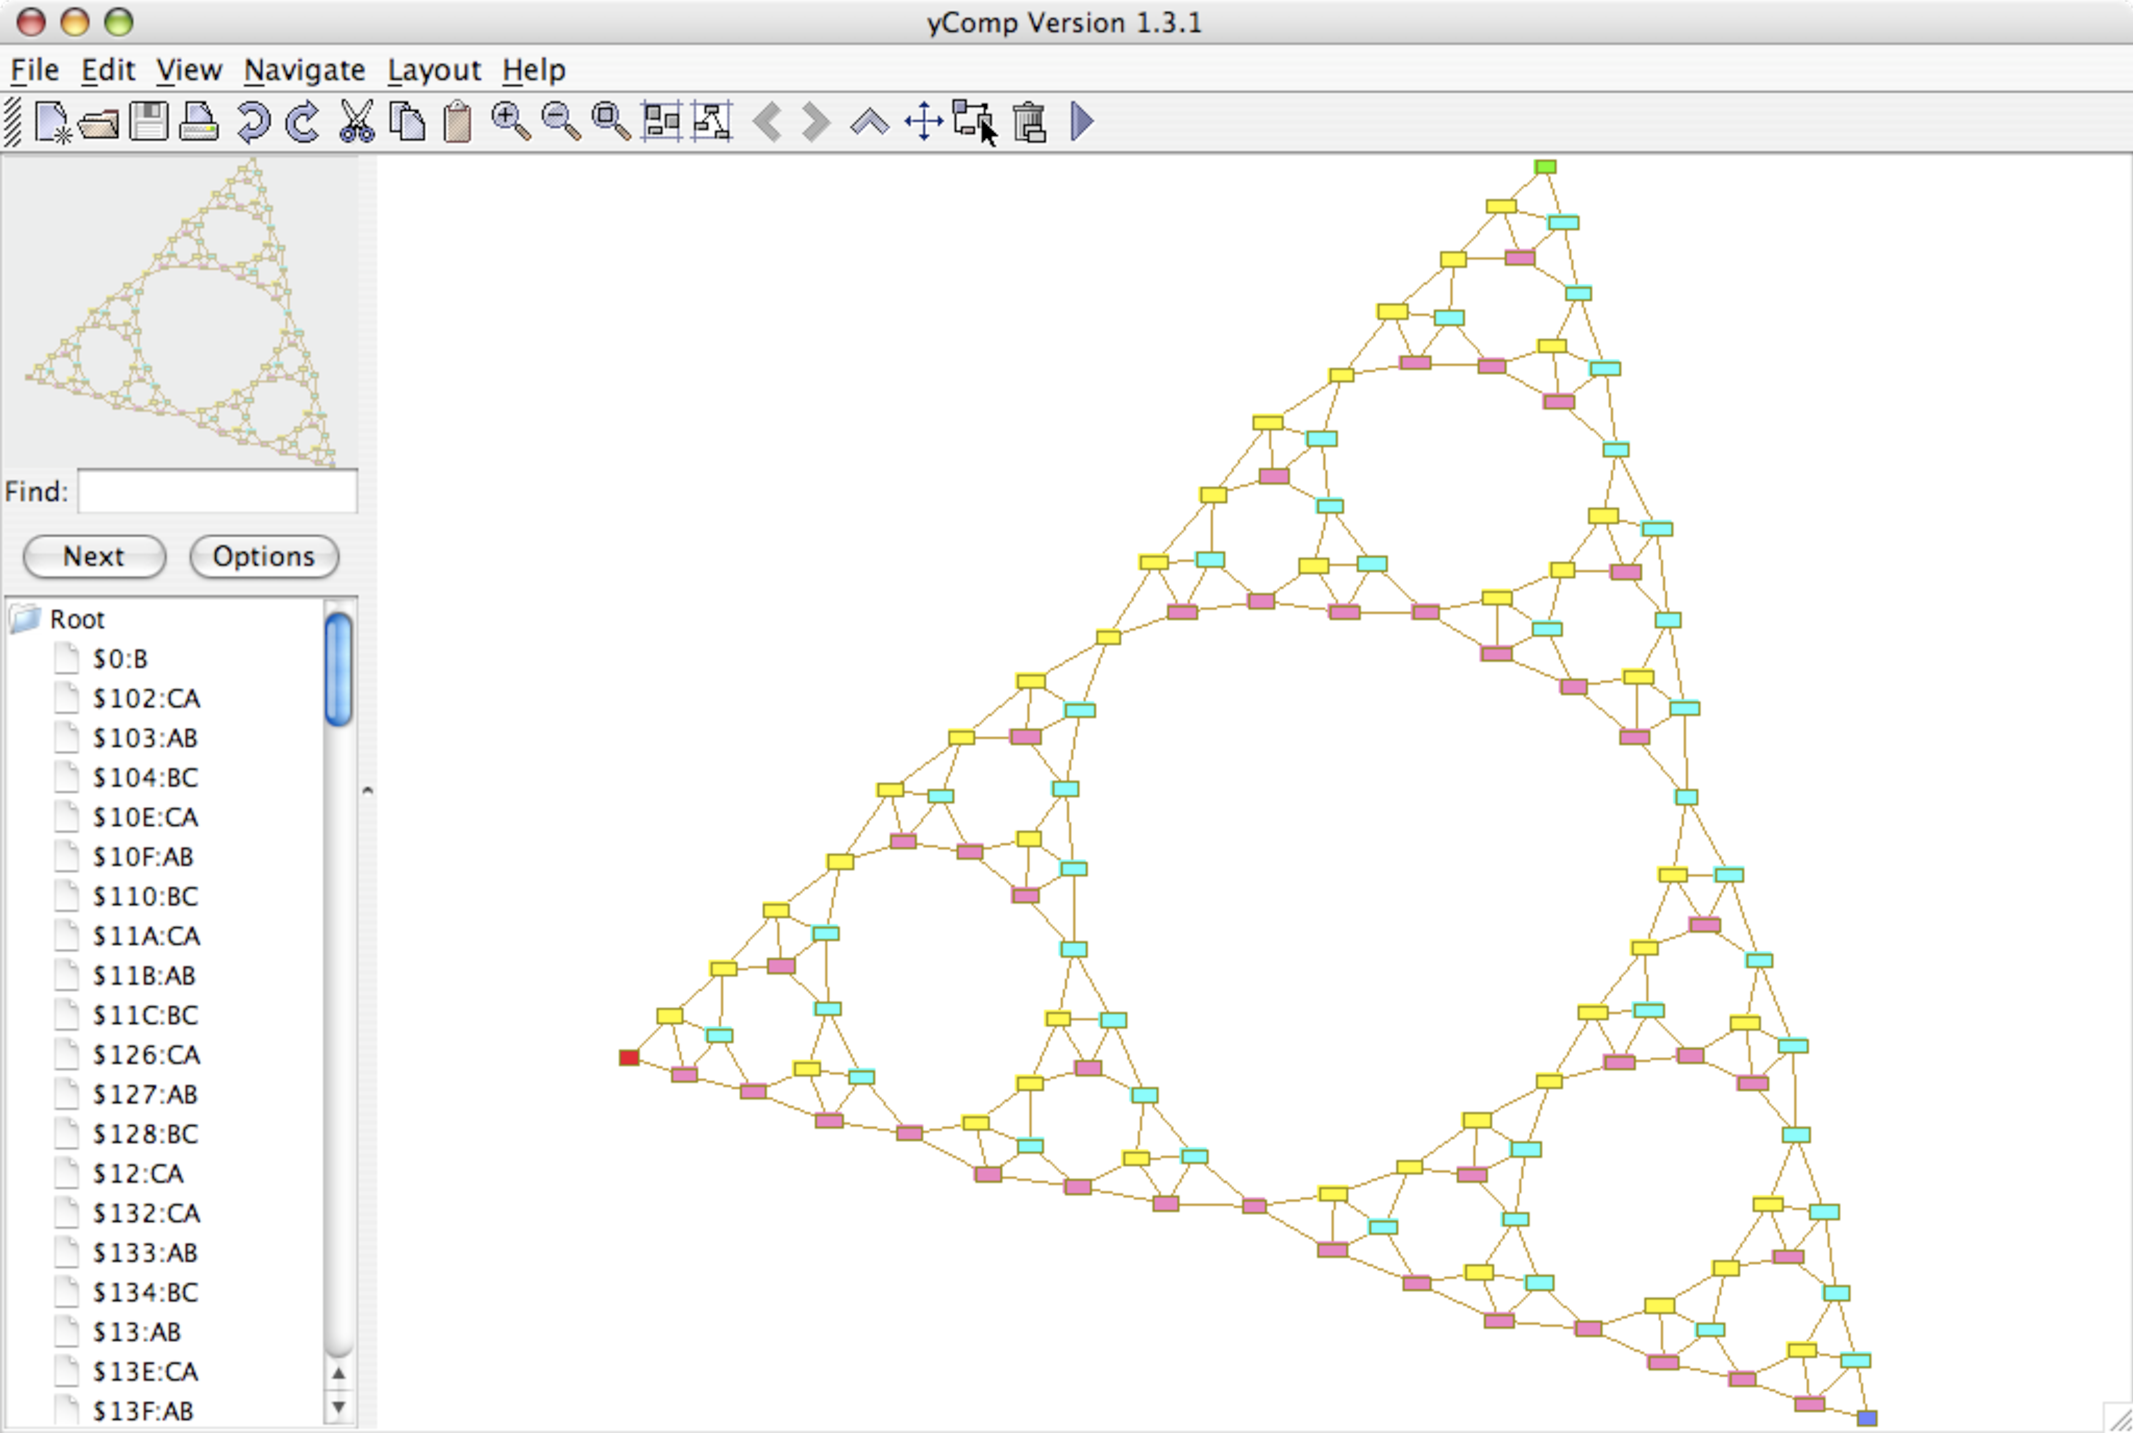
\includegraphics[width=\textwidth]{fig/sierpinski}
  \caption{Sierpinski triangle}
  \label{figsierp}
\end{figure}
\begin{figure}[htbp]
  \centering
  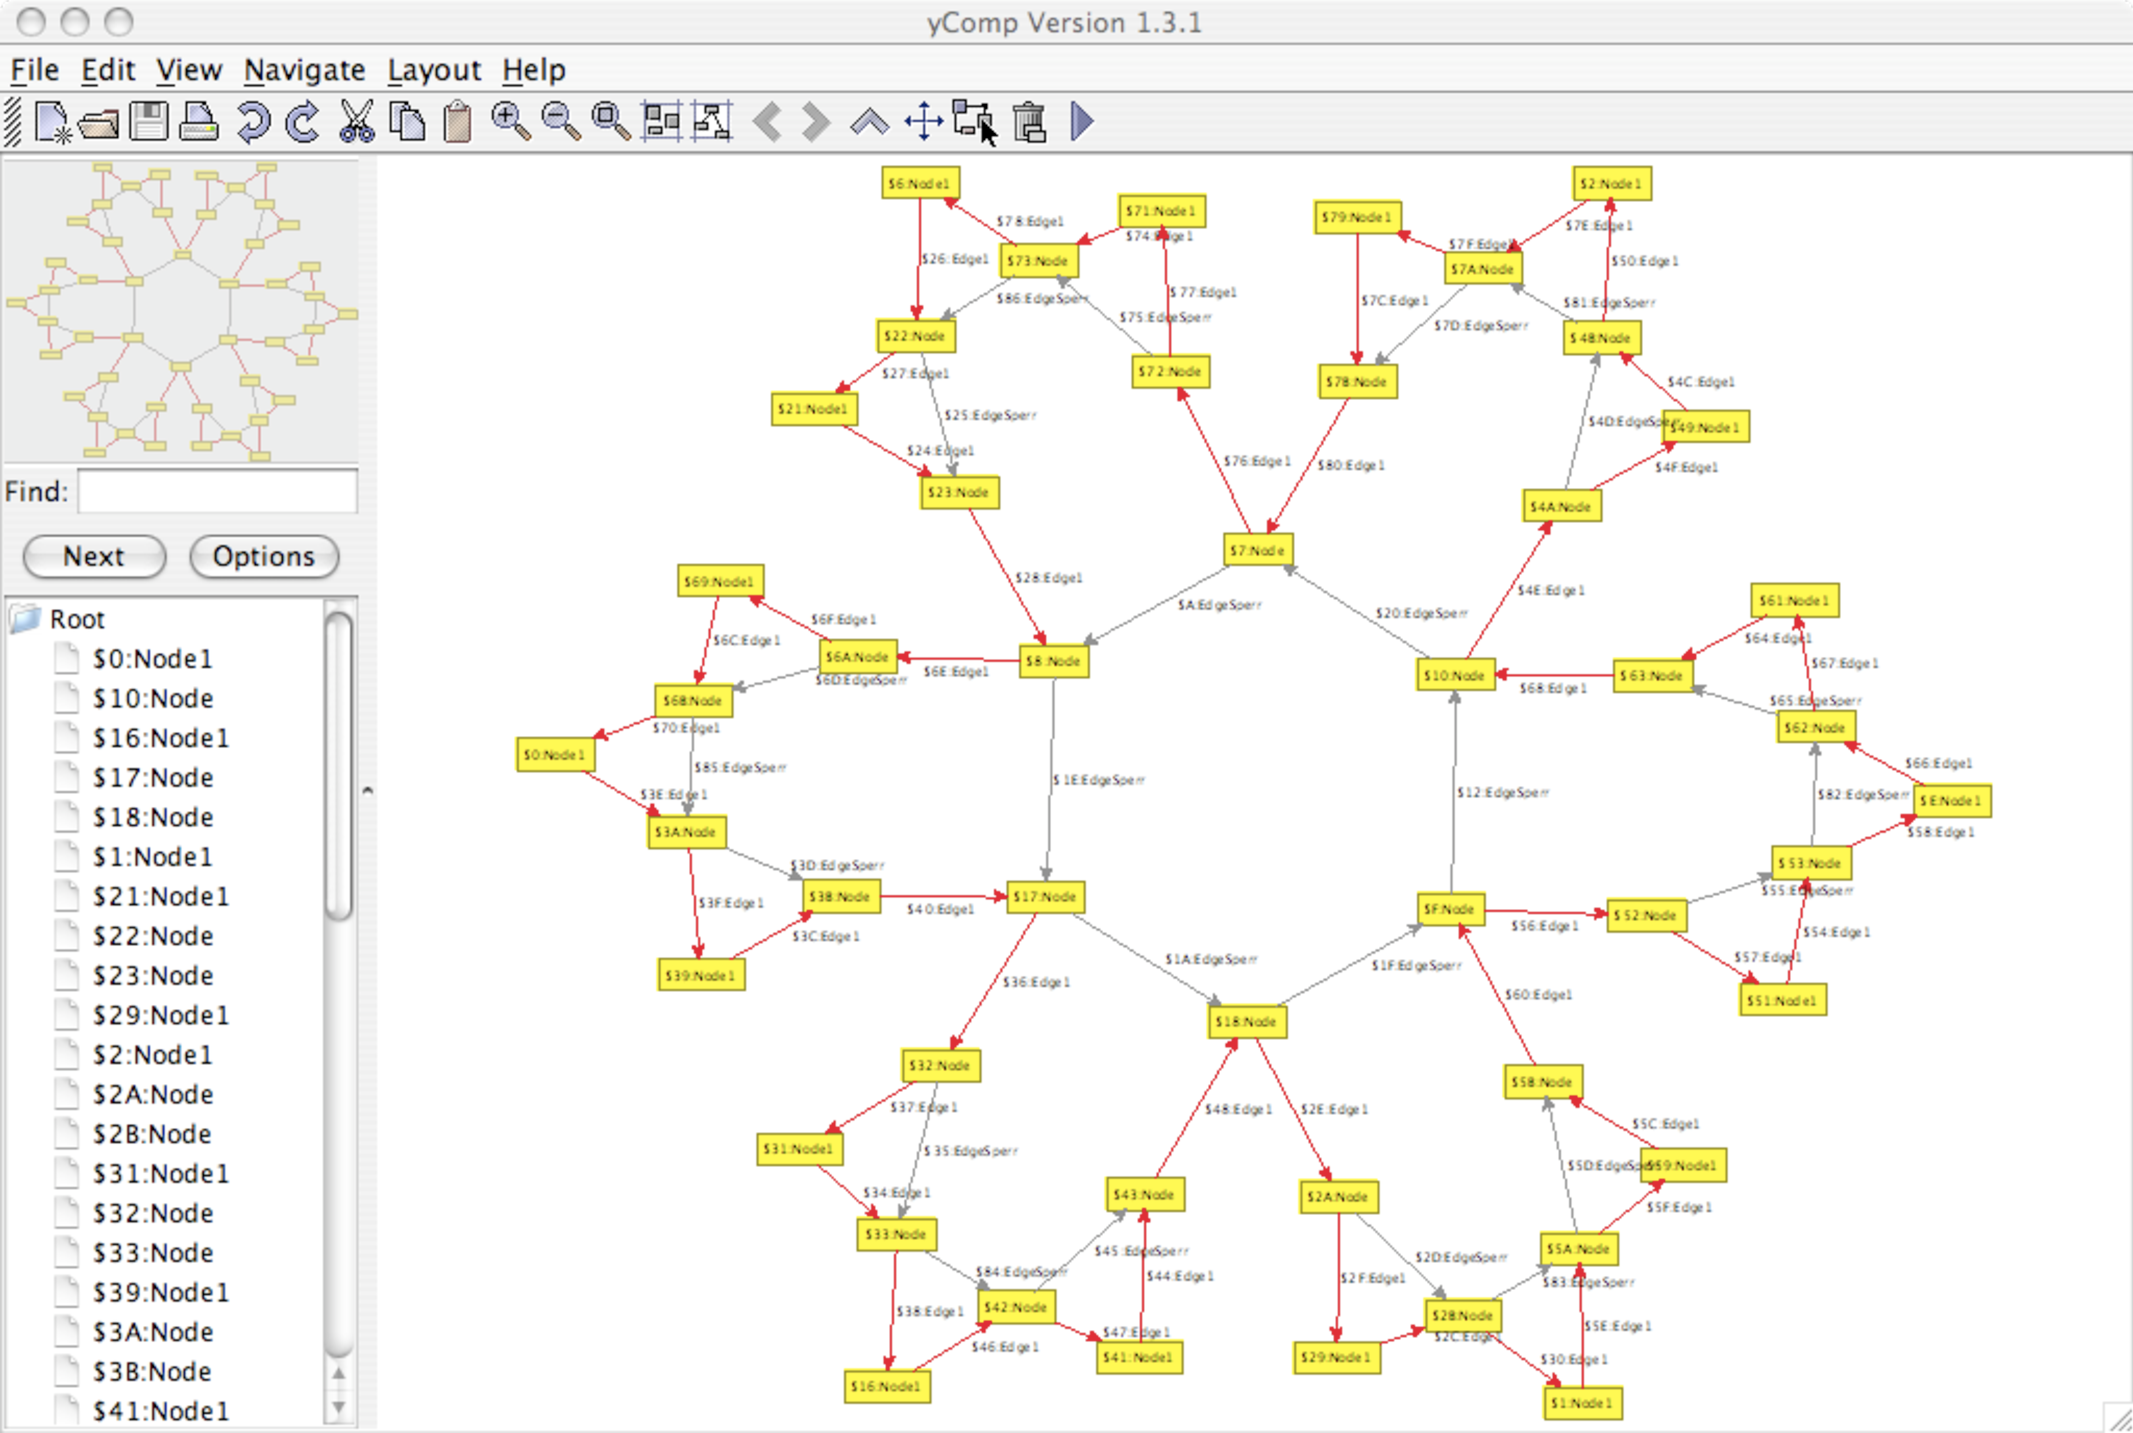
\includegraphics[width=\textwidth]{fig/snowflake}
  \caption{Koch snowflake}
  \label{figsnowflake}
\end{figure}
\vfill\pagebreak


%%%%%%%%%%%%%%%%%%%%%%%%%%%%%%%%%%%%%%%%%%%%%%%%%%%%%%%%%%%%%%%%%%%%%%%%%%%%%%%%%%%%%%%%%%%%%%%%
\section{Busy Beaver}\indexmain{example}
We want \GrG\ to work as hard as a \indexed{busy beaver}~\cite{Kro:07,Dew:84}. Our busy beaver is a Turing machine that has got five states plus a ``halt''-state; it writes 1,471 bars onto the tape and terminates~\cite{MB:00}. So first of all we design a Turing machine as graph model. Besides, this example shows that \GrG\ is \indexed{Turing complete}.

We use the graph model and the rewrite rules to define a general Turing machine. Our approach is to basically draw the machine as a graph. The busy beaver logic is implemented by rule applications in \GrShell.

%-----------------------------------------------------------------------------------------------
\subsection{Graph Model}
The tape will be a chain of \texttt{TapePosition} nodes connected by right edges. A cell value is modeled by a reflexive \texttt{value} edge, attached to a \texttt{TapePosition} node. The leftmost and the rightmost cells (\texttt{TapePosition}) do not have an incoming and outgoing edge respectively. Therefore we have the node constraint $[0:1]$.
\begin{grgen}[firstnumber=last]
node class TapePosition;
edge class right
  connect TapePosition[0:1] --> TapePosition[0:1];

edge class value
  connect TapePosition[1] --> TapePosition[1];
edge class zero  extends value;
edge class one   extends value;
edge class empty extends value;

\end{grgen}
Furthermore we need states and transitions.
The machine's current configuration is modeled with a \texttt{RWHead} edge pointing to a \texttt{TapePosition} node.
\texttt{State} nodes are connected with \texttt{WriteValue} nodes via \texttt{value} edges, a \texttt{moveLeft}/\texttt{moveRight}/\texttt{dontMove} edge leads from a \texttt{WriteValue} node to the next state (cf.~the picture on page \pageref{fig:bbstart}).
\begin{grgen}[firstnumber=last]
node class State;

edge class RWHead;

node class WriteValue;
node class WriteZero extends WriteValue;
node class WriteOne extends WriteValue;
node class WriteEmpty extends WriteValue;

edge class moveLeft;
edge class moveRight;
edge class dontMove;
\end{grgen}

%-----------------------------------------------------------------------------------------------
\subsection{Rule Set}
Now the rule set: We begin the rule set file \texttt{Turing.grg} with
\begin{grgen}[firstnumber=1]
using TuringModel;

\end{grgen}
We need rewrite rules for the following steps of the Turing machine:
\begin{enumerate}
  \item Read the value of the current tape cell and select an outgoing edge of the current state.
  \item Write a new value into the current cell, according to the sub type of the \texttt{WriteValue} node.
  \item Move the read-write-head along the tape and select a new state as current state.
\end{enumerate}
As you can see a transition of the Turing machine is split into two graph rewrite steps: Writing the new value onto the tape and performing the state transition. We need eleven rules: Three rules for each step (for ``zero'', ``one'', and ``empty'') and two rules for extending the tape to the left and the right, respectively.
\begin{grgen}[firstnumber=last]
rule readZeroRule {
	s:State -h:RWHead-> tp:TapePosition -:zero-> tp;
	s -:zero-> wv:WriteValue;
	modify {
		delete(h);
		wv -:RWHead-> tp;
	}
}

\end{grgen}
We take the current state \texttt{s} and the current cell \texttt{tp} which is implicitly given by the unique \texttt{RWHead} edge and check whether the cell value is zero. Furthermore we check if the state has a transition for zero. The replacement part deletes the \texttt{RWHead} edge between \texttt{s} and \texttt{tp} and adds it between \texttt{wv} and \texttt{tp}. The remaining rules are analogous:
\begin{grgen}[firstnumber=last]
rule readOneRule {
	s:State -h:RWHead-> tp:TapePosition -:one-> tp;
	s -:one-> wv:WriteValue;
	modify {
		delete(h);
		wv -:RWHead-> tp;
	}
}

rule readEmptyRule {
	s:State -h:RWHead-> tp:TapePosition -:empty-> tp;
	s -:empty-> wv:WriteValue;
	modify {
		delete(h);
		wv -:RWHead-> tp;
	}
}

rule writeZeroRule {
	wv:WriteZero -rw:RWHead-> tp:TapePosition -:value-> tp;
	replace {
		wv -rw-> tp -:zero-> tp;
	}
}

rule writeOneRule {
	wv:WriteOne -rw:RWHead-> tp:TapePosition -:value-> tp;
	replace {
		wv -rw-> tp -:one-> tp;
	}
}

rule writeEmptyRule {
	wv:WriteEmpty -rw:RWHead-> tp:TapePosition -:value-> tp;
	replace {
		wv -rw-> tp -:empty-> tp;
	}
}

rule moveLeftRule {
	wv:WriteValue -:moveLeft-> s:State;
	wv -h:RWHead-> tp:TapePosition <-r:right- ltp:TapePosition;
	modify {
		delete(h);
		s -:RWHead-> ltp;
	}
}

rule moveRightRule {
	wv:WriteValue -:moveRight-> s:State;
	wv -h:RWHead-> tp:TapePosition -r:right-> rtp:TapePosition;
	modify {
		delete(h);
		s -:RWHead-> rtp;
	}
}

rule dontMoveRule {
	wv:WriteValue -:dontMove-> s:State;
	wv -h:RWHead-> tp:TapePosition;
	modify {
		delete(h);
		s -:RWHead-> tp;
	}
}

rule ensureMoveLeftValidRule {
	wv:WriteValue -:moveLeft-> :State;
	wv -:RWHead-> tp:TapePosition;
	negative {
		tp <-:right-;
	}
	modify {
		tp <-:right- ltp:TapePosition -:empty-> ltp;
	}
}

rule ensureMoveRightValidRule {
	wv:WriteValue -:moveRight-> :State;
	wv -:RWHead-> tp:TapePosition;
	negative {
		tp -:right->;
	}
	modify {
		tp -:right-> rtp:TapePosition -:empty-> rtp;
	}
}
\end{grgen}
Have a look at the negative conditions within the \texttt{ensureMove\dots} rules. They ensure that the current cell is indeed at the end of the tape: An edge to a right/left neighboring cell must not exist. Now don't forget to compile your model and the rule set with \texttt{GrGen.exe} (see Section~\ref{fractals}).

%-----------------------------------------------------------------------------------------------
\subsection{Rule Execution with \GrShell}

Finally we construct the busy beaver and let it work with \GrShell. The following script starts with building the Turing machine that is modeling the six states with their transitions in our Turing machine model:
\begin{grshell}[firstnumber=1]
select backend "../bin/lgspBackend.dll"
new graph "../lib/lgsp-TuringModel.dll" "Busy Beaver"
select actions "../lib/lgsp-TuringActions.dll"

# Initialize tape
new tp:TapePosition($="Startposition")
new tp -:empty-> tp

# States
new sA:State($="A")
new sB:State($="B")
new sC:State($="C")
new sD:State($="D")
new sE:State($="E")
new sH:State($ = "Halt")

new sA -:RWHead-> tp

# Transitions: three lines per state and input symbol for
#   - updating cell value
#   - moving read-write-head
# respectively

new sA_0: WriteOne
new sA -:empty-> sA_0
new sA_0 -:moveLeft-> sB

new sA_1: WriteOne
new sA -:one-> sA_1
new sA_1 -:moveLeft-> sD

new sB_0: WriteOne
new sB -:empty-> sB_0
new sB_0 -:moveRight-> sC

new sB_1: WriteEmpty
new sB -:one-> sB_1
new sB_1 -:moveRight-> sE

new sC_0: WriteEmpty
new sC -:empty-> sC_0
new sC_0 -:moveLeft-> sA

new sC_1: WriteEmpty
new sC -:one-> sC_1
new sC_1 -:moveRight-> sB

new sD_0: WriteOne
new sD -:empty-> sD_0
new sD_0 -:moveLeft->sE

new sD_1: WriteOne
new sD -:one-> sD_1
new sD_1 -:moveLeft-> sH

new sE_0: WriteOne
new sE -:empty-> sE_0
new sE_0 -:moveRight-> sC

new sE_1: WriteOne
new sE -:one-> sE_1
new sE_1 -:moveLeft-> sC

\end{grshell}
\quad\\Our busy beaver looks like this:\label{fig:bbstart}
\begin{center}
  \fbox{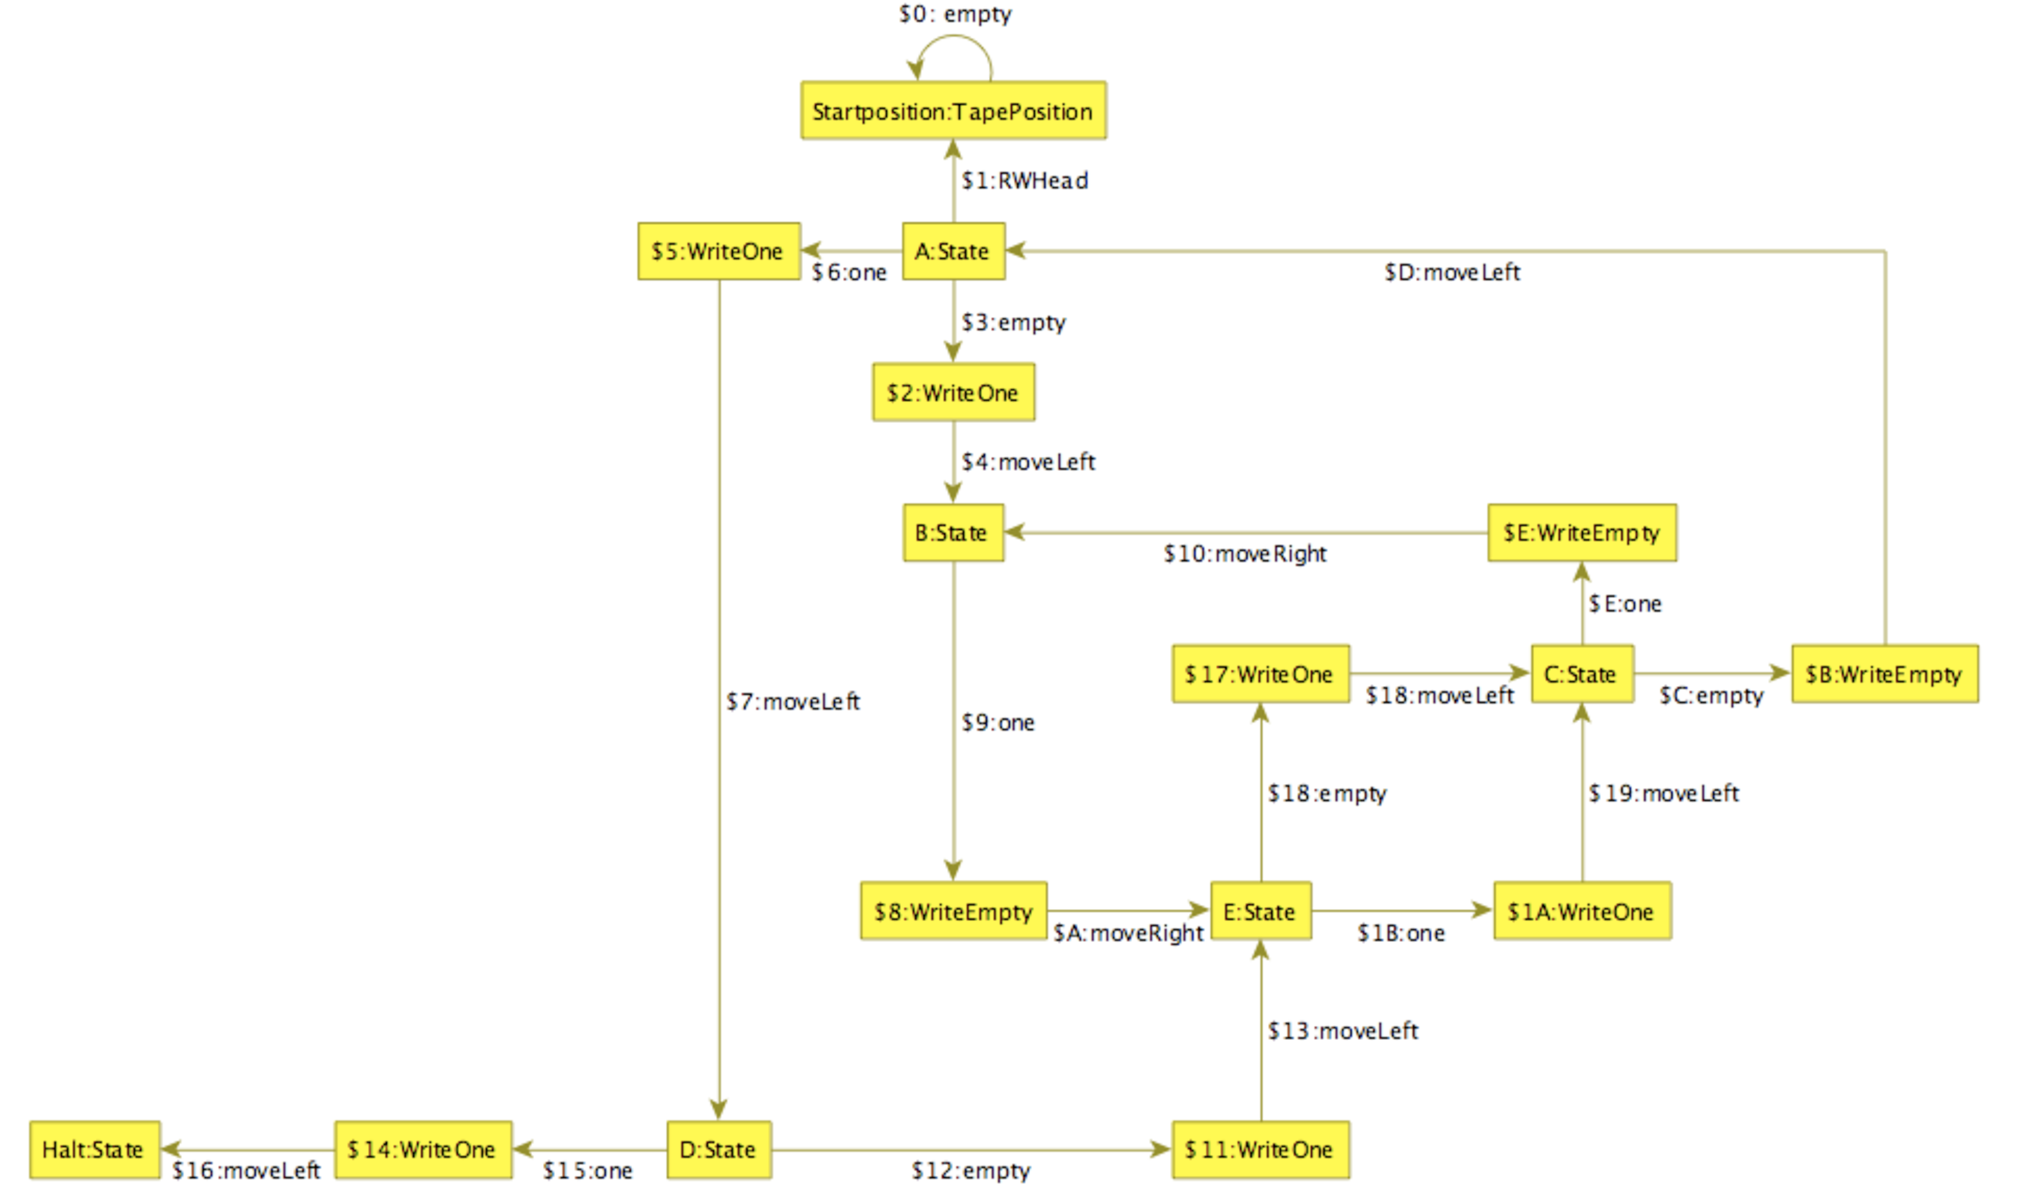
\includegraphics[width=\linewidth-2\fboxsep-2\fboxrule]{fig/bbstart}}
\end{center}

We have an initial host graph now. The graph rewrite sequence is quite straight forward and generic to the Turing graph model. Note that for each state the ``\texttt{\dots Empty\dots} | \texttt{\dots One\dots}'' selection is unambiguous.
%\pagebreak %HACK
\begin{grshell}[firstnumber=last]
  xgrs ((readOneRule | readEmptyRule) & (writeOneRule | writeEmptyRule) & (ensureMoveLeftValidRule | ensureMoveRightValidRule) & (moveLeftRule | moveRightRule))[32]

\end{grshell}
\quad\\We interrupt the machine after 32 iterations and look at the result so far:
\begin{center}
  \fbox{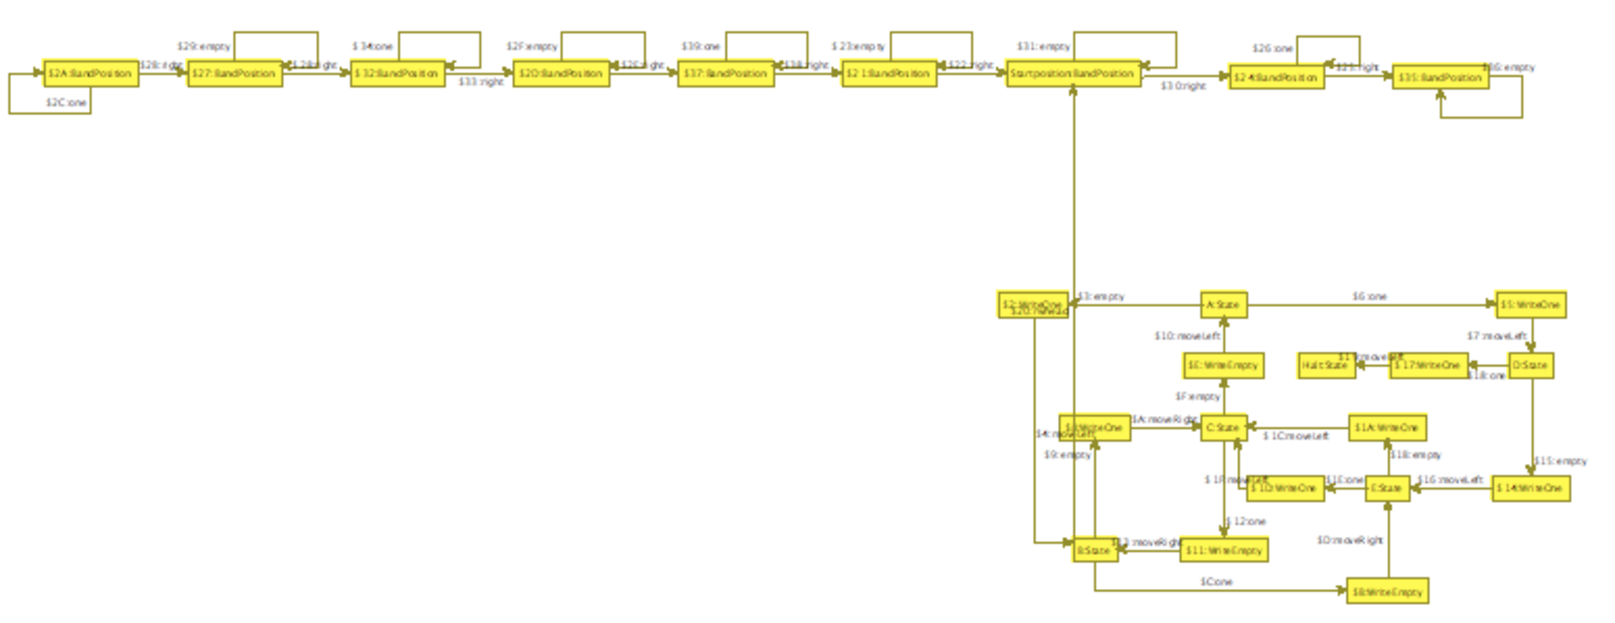
\includegraphics[width=\linewidth-2\fboxsep-2\fboxrule]{fig/bbmiddle}}
\end{center}
In order to improve the performance we generate better \indexed{search plan}s. This is a crucial step for execution time: With the initial search plans the beaver runs for 1 minute and 30 seconds. With improved search plans after the first 32 steps he takes about 8.5 seconds\footnote{On a Pentium 4, 3.2Ghz, with 2GiB RAM.}.
\begin{grshell}[firstnumber=last]
custom graph analyze_graph
custom actions gen_searchplan readOneRule readEmptyRule writeOneRule writeEmptyRule ensureMoveLeftValidRule ensureMoveRightValidRule moveLeftRule moveRightRule

\end{grshell}

Let the beaver run:
\begin{grshell}[firstnumber=last]
  xgrs ((readOneRule | readEmptyRule) & (writeOneRule | writeEmptyRule) & (ensureMoveLeftValidRule | ensureMoveRightValidRule) & (moveLeftRule | moveRightRule))*
\end{grshell}




\chapter{Application Programming Interface}\indexmainsee{application programming interface}{API} \indexmain{API}
\label{cha:api}

This chapter describes the Application Programming Interface of \GrG, i.e. of the system runtime - the LibGr - and of the assemblies generated from the model and rule specifications.
We'll have a look at
\begin{itemize}
\item the interface to the graph and model
\item the interface to the rules and matches
\item the interface of the graph processing environment
\item the porter module for importing and exporting of graphs and miscellaneous stuff
\item implementing external class and function declarations
\item implementing external match filter and external sequence declarations
\item events fired when the graph is changed
\item events fired during action execution
\end{itemize}

\noindent From the input file \texttt{Foo.grg} \texttt{grgen.exe} generates the output files \texttt{FooModel.cs} for the model and \texttt{FooActions.cs} for the actions,
\begin{itemize}
\item defining the exact interface, 
\item implementing the exact interface with generated code and code from the lgsp backend, i.e. entities from \texttt{de.unika.ipd.grGen.lgsp} available from lgspBackend.dll, 
\item and implementing the generic interface from \texttt{de.unika.ipd.grGen.libGr} using the entities mentioned in both points above.
\end{itemize}

\noindent This generative approach bears a great deal of the responsibility for the high execution speed of GrGen.NET, but it comes at the price of flexibility: you can't extend the rule set at runtime with new rules.
What you can do at runtime on the other hand is to generate a new rule set file, apply the compiler, and dynamically link the resulting assemblies/dlls.

When working with the API, you could reference the generated binary dlls in your project, in the same way as you have to reference the \texttt{libGr.dll} and \texttt{lgspBackend.dll}.
For easier debugging though, especially when you are integrating the generated code with own extensions (as described in chapter \ref{chapextensions}), it is recommended to directly include the source code generated (which is thrown away normally after it was compiled into the assemblies lgsp-FooModel.dll and lgsp-FooActions.dll).
For this, use the \texttt{-keep} option when you call \texttt{grgen.exe}, and include the model and the actions file (excluding the intermediate actions file) directly as C\# source code files.

The matcher code generated contains the initial, static search plans.
When you analyze the graph at runtime and generate new matchers, see section \ref{custom} for more on this, you can request the dumping of the source code of the improved matchers.
The custom commands are available at API level via the \texttt{Custom} operation of the \texttt{IGraph} interface for the graph commands and the \texttt{Custom} operation of the \texttt{BaseActions} class for the actions commands, just handing in the same parameters as otherwise specified on the command line.
If the intended workflow of ``i) loading a typical graph or doing a warm-up run creating a typical graph, ii) analyzing that graph, iii) compiling new matchers which are better suited to the graph'' is not easily achievable, or you want to start with the optimized matchers straight from the beginning, you may copy and paste the dumped dynamic matchers of an example run to the existing static code. 
But this is only a last resort, as the price is that your manual editing is overwritten again with the static search plans at the next time you call \texttt{grgen}.


%%%%%%%%%%%%%%%%%%%%%%%%%%%%%%%%%%%%%%%%%%%%%%%%%%%%%%%%%%%%%%%%%%%%%%%%%%%%%%%%%%%%%%%%%%%%%%%%
\section{Interface to the Host Graph}

The generated file \texttt{FooModel.cs} opens the namespace \texttt{de.unika.ipd.grGen.Model\_Foo} containing all the generated entities.
It contains for every node or edge class \texttt{Bar} an interface \texttt{IBar}, which offers C\# properties giving access to the attributes, and is inheriting in the same way as specified in the model file.
This builds the exact interface of the model, it is implemented by a sealed class \texttt{Bar} with generated code and with code from the lgsp backend.
Furtheron the namespace contains a model class \texttt{FooGraphModel} implementing the interface \texttt{de.unika.ipd.grGen.libGr.IGraphModel},
which supports iteration over the entities defined in the model using further, generic(i.e. inexact) interfaces from libGr.
Finally, the namespace contains a class \texttt{FooGraph} which defines an \texttt{LGSPGraph} of a model equivalent to \texttt{FooGraphModel}; 
it contains convenience functions to easily create nodes and edges of exact type in the graph.
In addition, a class \texttt{FooNamedGraph} is available, which defines an \texttt{LGSPNamedGraph} of a model equivalent to \texttt{FooGraphModel}; 
the named graph offers persistent names \ref{persistentex} for all its graph elements, otherwise it is identical to an \texttt{LGSPGraph}.
The naming requires about the same memory as an unnamed graph, but under normal circumstances the named graph is the recommended one to use (and is the one which will be used if employed by the shell).

\begin{note}
If you want to use the type-safe interface, use the interface \texttt{IBar}, and the \texttt{CreateNodeBar}-methods of \texttt{FooGraph} or the \texttt{CreateNode}-method of \texttt{Bar}.
If you want to use the generic interface, your entry point is the \texttt{IGraphModel}, with \texttt{INodeModel.GetType("Bar")} returning a \texttt{NodeType}, used in \texttt{IGraph.AddNode(NodeType)} returning an \texttt{INode}.
\end{note}


%%%%%%%%%%%%%%%%%%%%%%%%%%%%%%%%%%%%%%%%%%%%%%%%%%%%%%%%%%%%%%%%%%%%%%%%%%%%%%%%%%%%%%%%%%%%%%%%
\section{Interface to the Rules}

The generated file \texttt{FooActions.cs} opens the \texttt{namespace de.unika.ipd.grGen.Action\_Foo} containing all the generated entities.
It contains for every rule or test \texttt{bar}
\begin{itemize}
\item a class \texttt{Rule\_bar} inheriting from \texttt{de.unika.ipd.grGen.lgsp.LGSPRulePattern}, which contains
the exact match interface \texttt{IMatch\_bar} which defines how a match of the rule looks like,
extending the generic rule-unspecific \texttt{IMatch} interface.
Have a look at section \ref{sub:extflt} for an extended introduction to the matches interfaces. 
Furtheron there are (but meant only for internal use): a match class \texttt{Match\_bar} implementing the exact and inexact interface,
a description of the pattern to match, and the modify methods doing the rewriting.
\item an exact action interface \texttt{IAction\_bar} which contains the methods:
  \begin{itemize}
  \item \texttt{Match}, to match the pattern in the host graph,
     with in-parameters corresponding to the in-parameters of the rule (name and type),
	 returning matches of the exact type \texttt{Rule\_bar.IMatch\_bar}.
  \item \texttt{Modify}, to modify a given match according to the rewrite specification,
     with out-parameters corresponding to the out-parameters of the rule.
  \item \texttt{Apply}, to match and modify the found match,
     with in-parameters corresponding to the in-parameters of the rule,
     and with ref-parameters corresponding to the out-parameters of the rule.
  \end{itemize}
  Furtheron there is (but meant only for internal use) the class \texttt{Action\_bar} implementing the exact action interface as well as the generic \texttt{IAction} interface from libGr;
  it contains the generated matcher code searching for the patterns.
\end{itemize}

Moreover the namespace contains an action class \texttt{FooActions}
implementing the abstract class \texttt{de.unika.ipd.grGen.libGr.BaseActions} (in fact \texttt{de.unika.ipd.grGen.lgsp.LGSPActions}),
which supports iteration over the entities defined in the actions using further, generic(i.e. inexact) interfaces from libGr.
Additionally, at runtime it contains the instances of the actions singletons,
as member \texttt{bar} of the exact type \texttt{IAction\_bar}.
\begin{note}
If you want to use the type-safe interface, your entry point is the member \texttt{bar} of type \texttt{IAction\_bar} from \texttt{FooActions} (or \texttt{Action\_bar.Instance}).
Actions are used with named parameters of exact types.
If you want to use the generic interface, your entry point is the method \texttt{GetAction("bar")} of the interface \texttt{BaseActions} implemented by \texttt{FooActions} returning an \texttt{IAction}.
Actions are used with \texttt{object}-arrays for parameter passing.
\end{note}

\begin{note}
The old generic interface of string names and entities of node-,edge-, and object-type is implemented with the new interface of exactly typed, named entities.
Thus you will receive runtime exceptions when doing operations which are not type-safe with the generic interface, in contrast to \GrG\ $<$ v2.5.
If you need the flexibility of the old input parameters semantics of silently failing rule application on a wrong type,
you must declare it explicitly with the syntax \verb#r(x:ExactType<InexactType>)#;
then the rule parameter in the exact interface will be of type \texttt{InexactType}.
\end{note}

\begin{example}\label{ex:api1}
Normally you want to use the type-safe interface of the generated code as it is much more convenient.
Only if your application must get along with models and actions unknown before it is compiled you have to fall back to the generic interface.
An extensive example showing how to cope with the latter is shipped with \GrG\ in form of the GrShell.
Here we'll show a short example on how to use \GrG\ with the type-safe API; 
further examples are given in the examples-api folder of the \GrG-distribution.

We'll start with including the namespaces of the libGr and the lgsp backend shipped with \GrG\,
plus the namespaces of our actions and models, generated from \texttt{Foo.grg}.
\begin{verbatim}
using de.unika.ipd.grGen.libGr;
using de.unika.ipd.grGen.lgsp;
using de.unika.ipd.grGen.Action_Foo;
using de.unika.ipd.grGen.Model_Foo;
\end{verbatim}

Then we create a graph with model bound at generation time and create actions to operate on this graph.
Afterwards we create a single node of type \texttt{Bar} in the graph and save it to the variable \texttt{b}.
Finally we apply the action \texttt{bar(Bar x) : (Bar)} to the graph with \texttt{b} as input receiving the output as well.
The rule is taken from the actions via the member named as the action.
\begin{verbatim}
FooGraph graph = new FooGraph();
FooActions actions = new FooActions(graph);
Bar b = graph.CreateNodeBar();
actions.bar.Apply(graph, b, ref b); // input of type Bar, output of type Bar
\end{verbatim}

We could create a named graph instead offering persistent names for its graph elements:
\begin{verbatim}
FooNamedGraph graph = new FooNamedGraph();
\end{verbatim}
\end{example}

\begin{example}
This is an example doing mostly the same as the previous example \ref{ex:api1}, in a slightly more complicated way allowing for more control.
Here we create the model separate from the graph, then the graph with a model not bound at generation time.
We create the actions to apply on the graph, and a single node of type \texttt{Bar} in the graph, which we assign again to a variable \texttt{b}.
Then we get the action from the actions and save it to an action variable \texttt{bar};
afterwards we use the action for finding all available matches of \texttt{bar} with input \texttt{b} -- which is different from the first version -- and remember the found matches in the matches variable with its exact type.
Finally we take the first match from the matches and execute the rewrite with it.
We could have inspected the nodes and edges of the match or their attributes before (using element names prefixed with \texttt{node\_/edge\_} or attribute names to get exactly typed entities). 
\begin{verbatim}
IGraphModel model = new FooGraphModel();
LGSPGraph graph = new LGSPGraph(model);
FooActions actions = new FooActions(graph);
Bar b = Bar.CreateNode(graph);
IAction_bar bar = Action_bar.Instance;
IMatchesExact<Rule_bar.IMatch_bar> matches = bar.Match(graph, 0, b);
bar.Modify(graph, matches.First);
\end{verbatim}

We could create a named graph instead offering persistent names for its graph elements:
\begin{verbatim}
LGSPGraph graph = new LGSPNamedGraph(model);
\end{verbatim}
\end{example}

%%%%%%%%%%%%%%%%%%%%%%%%%%%%%%%%%%%%%%%%%%%%%%%%%%%%%%%%%%%%%%%%%%%%%%%%%%%%%%%%%%%%%%%%%%%%%%%%
\section{Interface of the Graph Processing Environment}

The interface \texttt{IGraphProcessingEnvironment} implemented by the \texttt{LGSPGraphProcessing\-Environment} class offers all the additional functionality of \GrG~exceeding what is offered by the graph and the actions.
It is constructed as \texttt{LGSPGraphProcessingEnvironment} given the graph and the actions.
It offers execution of the sequences and variable handling, combining actions into transformations
(the former regarding control flow, the latter regarding data flow).

\begin{example}\label{ex:procenv}
For all but the simplest transformations you'll end up constructing a graph processing environment from the graph and the actions constructed until now, executing a graph rewrite sequence on the graph processing environment:
\begin{verbatim}
LGSPGraphProcessingEnvironment procEnv = 
    new LGSPGraphProcessingEnvironment(graph, actions);
procEnv.ApplyGraphRewriteSequence("<(::x)=foo && (::y)=bar(::x) | bla(::y)>");
\end{verbatim}
\end{example}

In addition to sequences and variables handling, the graph processing environment offers driver or helper objects for transaction management, deferred sequence execution, graph change recording, and emitting.
The most important of these is the transaction manager which is utilized when \GrG~ is used for crawling through a search space or for enumerating a state space, see section \ref{sec:extctrl}.
The operations mentioned there are implemented by calling the function given in example \ref{ex:transman}.

\begin{example}\label{ex:transman}
\begin{verbatim}
LGSPGraphProcessingEnvironment procEnv = ...;
ITransactionManager tm = procEnv.TransactionManager;
public interface ITransactionManager
{
    int Start();
    void Pause();
    void Resume();
    void Commit(int transactionID);
    void Rollback(int transactionID);
}
\end{verbatim}
\end{example}

The \texttt{Start} starts a transaction and returns its id; it may be called multiple times returning different ids for the then nested transactions (i.e. a failing outer one rolls back the changes of an inner transaction which succeeded).
Changes to the graph are recorded thereafter into an undo log, unless a \texttt{Pause} was called not yet followed by a \texttt{Resume}.
When the changes of interest were carried out the transaction identified by its id is either \texttt{Commit}ed, which causes the changes recorded since the corresponding \texttt{Start} to stay in the graph, or rolled back by calling \texttt{Rollback}, in that case all the changes recorded since the corresponding \texttt{Start} are undone.

%%%%%%%%%%%%%%%%%%%%%%%%%%%%%%%%%%%%%%%%%%%%%%%%%%%%%%%%%%%%%%%%%%%%%%%%%%%%%%%%%%%%%%%%%%%%%%%%
\section{Import/Export and Miscellaneous Stuff}\label{sub:imexport}\indexmain{import}\indexmain{export}

GrGen natively supports the following formats:
\begin{description}
  \item[GRS/GRSI] Reduced GrShell script files (graph only, model from \texttt{.gm}; a very limited version of the normal \texttt{.grs}. The recommended standard format.)
  \item[GXL] Graph eXchange Language (\texttt{.gxl}-files, see \url{http://www.gupro.de/GXL/})
  \item[ECORE/XMI] Ecore(\texttt{.ecore}) model files and XMI(\texttt{.xmi}) graph file. Import only, export must be programmed with \texttt{emit}-statements. In an intermediate step, a \texttt{.gm} file is generated for the model.
    \item[GRG] Writes a GrGen rule file containing one rule with an empty pattern and a large rewrite part. Export only \footnote{Original German Pisswasser, for export only :)}, not for normal use.
\end{description}

While both GRS and GXL importers expect one file
(the GXL importer allows to specify a model override, see GrShell import, Note \ref{shellgxlimport}),
the EMF/ECORE importer expects first one or more \texttt{.ecore} files
and following optionally a \texttt{.xmi} files and/or a \texttt{.grg} file (cf. Note \ref{shellecoreexport}). 
To use additional custom graph models you should supply an own \texttt{.grg}
file which may be based on the automatically generated \texttt{.grg} file, if none was
supplied (see the Program-Comprehension example in \texttt{examples/ProgramComprehension-GraBaTs09}).

To import a graph model and/or a graph instance you can use \texttt{Porter.Import()} from the libGr API (the GrShell command \texttt{import} is mapped to it)
The file format is determined by the file extensions.
To export a graph instance you can use \texttt{Porter.Export()} from the libGr API (the GrShell command \texttt{export} is mapped to it).
For an example of how to use the importer/exporter on API level see \texttt{examples-api/JavaProgramGraphsExample/JavaProgramGraphs\-Example.cs}

The GRS(I) importer returns an \texttt{INamedGraph};
if you don't need the persistent names, get rid of them by casting to the \texttt{LGSPNamedGraph} implementing the interface, (copy-)constructing a \texttt{LGSPGraph} from it, and forgetting any references to the named graph.
Please be aware that naming is rather expensive:
A \texttt{LGSPNamedGraph} supplying the name to element and element to name mappings normally uses up about twice the amount of memory of the \texttt{LGSPGraph} defining the graph alone (but is worth is most often).

\subsection*{External Emitting and Parsing}\label{sub:apiextemitparse}
If \texttt{emit class;} (see \ref{sub:extemitparse}) is specified in the model file \texttt{Foo}, \GrG~generates a file \texttt{FooModelExternalFunctions.cs} located besides the model and rule files,
containing the following functions.

\begin{csharplet}
/// <summary>
/// Called during .grs import, at exactly the position in the text reader where the attribute begins.
/// For attribute type object or a user defined type, which is treated as object.
/// The implementation must parse from there on the attribute type requested.
/// It must not parse beyond the serialized representation of the attribute, 
/// i.e. Peek() must return the first character not belonging to the attribute type any more.
/// Returns the parsed object.
/// </summary>
object Parse(TextReader reader, AttributeType attrType, IGraph graph);

/// <summary>
/// Called during .grs export, the implementation must return a string representation for the attribute.
/// For attribute type object or a user defined type, which is treated as object.
/// The serialized string must be parseable by Parse.
/// </summary>
string Serialize(object attribute, AttributeType attrType, IGraph graph);

/// <summary>
/// Called during debugging or emit writing, the implementation must return a string representation for the attribute.
/// For attribute type object or a user defined type, which is treated as object.
/// The attribute type may be null.
/// The string is meant for consumption by humans, it does not need to be parseable.
/// </summary>
string Emit(object attribute, AttributeType attrType, IGraph graph);
\end{csharplet}

\texttt{Parse} is called when an attribute of an external or object type is to be imported from a grs file, \texttt{Serialize} is called when an attribute of an external or object type is to be exported to a grs file, and \texttt{Emit} is called when a value of external or object type is to be emitted, or displayed in the debugger, including yComp.
(The functions are called from GrShell, too, insofar as possible -- the shell parses a single or double quoted text or a word or a number at an attribute position and hands that over then to the user defined parser.)
They forward the calls to \texttt{ParseImpl}, \texttt{SerializeImpl}, and \texttt{EmitImpl} functions, that need to be implemented in a file named \texttt{FooModelExternal\-FunctionsImpl.cs} located in the folder of the \texttt{FooModelExternalFunctions.cs} file.
Implementing them is \emph{your} task, in exchange you get a tight integration of your own datatypes into \GrG.
You may have a look at \texttt{tests/ExternalAttributeEvaluation} or  \texttt{examples\-api/ExternalAttributeEvaluationExample} for an example.


\subsection*{External Copying and Comparing}\label{sub:apiextcopycompare}
If \texttt{copy class;} or \texttt{== class;} or \texttt{< class;} (see \ref{sub:extcopycompare}) are specified in the model file \texttt{Foo},
\GrG~generates a file \texttt{FooModelExternalFunctions.cs} located besides the model and rule files,
containing a partial class \texttt{AttributeTypeObjectCopierComparer} expecting that the \texttt{Copy} or the \texttt{IsEqual} or the \texttt{IsLower} functions are implemented in the same partial class in \texttt{FooModelExternalFunctionsImpl.cs}.
For every external type defined a further pair of functions with that type used in the input parameters is expected.

\begin{csharplet}
// Called when a graph element is cloned/copied.
// For attribute type object.
// If "copy class" is not specified, objects are copied by copying the reference, i.e. they are identical afterwards.
// All other attribute types are copied by-value (so changing one later on has no effect on the other).
public static object Copy(object);

// Called during comparison of graph elements from graph isomorphy comparison, or attribute comparison.
// For attribute type object.
// If "== class" is not specified, objects are equal if they are identical,
// i.e. by-reference-equality (same pointer); all other attribute types are compared by-value.
public static bool IsEqual(object, object);

// Called during attribute comparison.
// For attribute type object.
// If "< class" is not specified, objects can't be compared for ordering, only for equality.
public static bool IsLower(object, object);
\end{csharplet}

\texttt{Copy} is called when one of the copy operations offered in the rule language or the computation statements is executed on a node or edge that bears attributes of object or user defined type.
\texttt{IsEqual} is called when two graphs are compared for isomorphy and the graph elements contain attributes of object or user-defined external types, or if attributes of object or user defined type are compared with one of the equality operators.
\texttt{IsLower} is called when attributes of object or user defined type are compared with one of the relational operators.
A comparison for \texttt{u<=v} is mapped to an expression \verb#IsLower(u,v) || IsEqual(u,v)#, this is why a \verb#< class;# specification requires a preceding \verb#== class;# specification.

Implementing those functions is \emph{your} task, in exchange you get a tight integration of your own datatypes into \GrG.
You may have a look at \texttt{tests/ExternalAttributeEvaluation} or  \texttt{examples\-api/ExternalAttributeEvaluationExample} for an example.

\subsection*{Further Examples}
There are further examples available in the \texttt{examples-api} folder of the \GrG-distribution:
\begin{itemize} 
\item How to use the graph rewrite sequences offered by the libGr on API level is shown in\\
\texttt{examples-api/BusyBeaverExample/BusyBeaverExample.cs}.\\
But normally you want to use your favourite .NET programming language for control together with the type-safe interface when working on API level.
\item How to use the old and new interface for accessing a match on API level is shown in\\
\texttt{examples-api/ProgramGraphsExample/ProgramGraphsExample.cs}.
\item How to use the visited\label{apiallocvisitflag} flags on API level is shown in\\
\texttt{examples-api/VisitedExample/VisitedExample.cs}.
\item How to analyze the graph and generate (hopefully) better performing matchers based on this information is shown in\\
\texttt{examples-api/BusyBeaverExample/BusyBeaverExample.cs}.
\item How to compile a \texttt{.grg}-specification at runtime and dump a graph for visualization in \texttt{.vcg} format on the API level is shown in\\
\texttt{examples-api/HelloMutex/HelloMutex.cs}.
\item How to access the annotations at API level is shown in\\
\texttt{examples-api/MutexDirectExample/MutexDirectExample.cs}.
\item How to communicate with yComp on the API level (from your own code) is shown in\\
\texttt{examples-api/YCompExample/YCompExample.cs} (it may be outdated, you better take a look at \texttt{GrShell/YCompClient.cs} for the real version).
\end{itemize}

\begin{warning}
While C\# allows input arguments values to be of a subtype of the declared interface parameter type (OO), 
it requires that the argument variables for the \texttt{out} parameters are of exactly the type declared (non-OO).
Although a variable of a supertype would be fully sufficient -- the variable is only assigned.
So for \texttt{node class Bla extends Bar;} and action \texttt{bar(Bar x) : (Bla)} from the rules file rules \texttt{Foo.grg}
we can't use a desired target variable of type \texttt{Bar} as \texttt{out}-argument,
but are forced to introduce a temporary variable of type \texttt{Bla}
and assign this variable to the desired target variable after the call.
\begin{csharplet}
using de.unika.ipd.grGen.libGr;
using de.unika.ipd.grGen.lgsp;
using de.unika.ipd.grGen.Action_Foo;
using de.unika.ipd.grGen.Model_Foo;
FooGraph graph = new FooGraph();
FooActions actions = new FooActions(graph);
Bar b = graph.CreateNodeBar();
IMatchesExact<Rule_bar.IMatch_bar> matches = actions.bar.Match(graph, 1, b);
//actions.bar.Modify(graph, matches.First, out b); // wont work, needed:
Bla bla = null; 
actions.bar.Modify(graph, matches.First, out bla);
b = bla;
\end{csharplet}
\end{warning}


%%%%%%%%%%%%%%%%%%%%%%%%%%%%%%%%%%%%%%%%%%%%%%%%%%%%%%%%%%%%%%%%%%%%%%%%%%%%%%%%%%%%%%%%%%%%%%%%
\section{External Class, Function and Procedure Implementation}\label{sub:extclsfctimpl}\indexmain{external class implementation}\indexmain{external function implementation}\indexmain{external procedure implementation}

For a model file \texttt{Foo} which contains external functions (cf. \ref{sub:extfct}) and/or classes (cf. \ref{sub:extcls}), \GrG~generates a file \texttt{FooModelExternalFunctions.cs} located besides the model and rule files, which contains
\begin{itemize}
	\item within the model namespace public partial classes named as given in the external class declaration,
inheriting from each other as stated in the external class declarations.
	\item within the \texttt{de.unika.ipd.grGen.expression} namespace a public partial class named \texttt{ExternalFunctions} with a body of comments giving the expected function and procedure prototypes.
\end{itemize}

\noindent The partial classes are empty, you must implement them in a file named \texttt{FooModelExternal\-FunctionsImpl.cs} located in the folder of the \texttt{FooModelExternalFunctions.cs} file by
\begin{itemize}
	\item fleshing out the partial classes skeletons with attributes containing data of interest and maybe helper methods
	\item fleshing out the \texttt{ExternalFunctions} partial class skeleton with the functions you declared in the external function declarations, obeying the function signatures as specified; here you can access the now know attributes or methods of the external classes, or do complicated custom computations or graph querying with the values you receive from a function call.
	\item fleshing out the \texttt{ExternalProcedures} partial class skeleton with the procedures you declared in the external procedure declarations, obeying the procedure signatures as specified; here you can access the now know attributes or methods of the external classes, or do complicated custom computations or graph manipulations with the values you receive from a procedure call.
\end{itemize}

\noindent Don't forget that the source code file \texttt{FooModelExternalFunctionsImpl.cs} is an integral part of your \GrG~graph transformation project, in contrast to the other C\# files generated (and overwritten) for you.
In \texttt{examples/ExternalAttributeEvaluationExample} and \texttt{examples-api/ExternalAttributeEvaluationExample}
you find a fabricated example showing how to use the external classes and functions.

When you use third-party assemblies in your source code you must inform GrGen.NET about them so references to them are included into the assembly generated; this can be done with the \texttt{-r} parameter when calling \texttt{grgen.exe} directly (cf. \ref{grgenoptions}) or with the \texttt{new} command configurations available in GrShell (cf. \ref{graphcommands}). Using the \texttt{keepdebug} configuration of the \texttt{new} command is recommended as it allows for easier debugging.


%%%%%%%%%%%%%%%%%%%%%%%%%%%%%%%%%%%%%%%%%%%%%%%%%%%%%%%%%%%%%%%%%%%%%%%%%%%%%%%%%%%%%%%%%%%%%%%%
\section{External Filter and Sequence Implementation}\label{sub:extfltseqimpl}\indexmain{external match filter implementation}\indexmain{external sequence implementation}

For an actions file \texttt{Bar} which contains match filter declarations (cf. \ref{sub:extflt}) and/or external sequence declarations (\ref{sub:extseq}), \GrG~generates a file \texttt{BarActionsExternalFunctions.cs} located besides the model and rule files, which contains within the action namespace 
\begin{itemize}
	\item a public partial class named \texttt{MatchFilters} with a body of comments giving the expected function prototypes, and for the \texttt{auto} filters even the implementation.
	\item public partial classes, named \texttt{Sequence\_foo} for a sequence \texttt{foo}, with a body containing a comment specifying the expected function prototype of the sequence application function.
\end{itemize}

\noindent The partial classes are empty, you must implement them in a file named \texttt{BarActionsExternal\-FunctionsImpl.cs} located in the folder of the \texttt{BarActionsExternalFunctions.cs} file by
\begin{itemize}
	\item fleshing out the \texttt{MatchFilters} partial class skeleton with the match filter functions you declared, obeying the function signatures as specified; you might want to convert the received matches object to an \texttt{IList} in case you want to reorder the list and reinject it into the matches object afterwards.
	\item fleshing out the partial classes skeletons of the external sequence with the \texttt{ApplyXGRS\_foo} methods needed.
\end{itemize}

\noindent Don't forget that the source code file \texttt{BarActionsExternalFunctionsImpl.cs} is an integral part of your \GrG~graph transformation project, in contrast to the other C\# files generated (and overwritten) for you.
In \texttt{examples/ExternalFiltersAndSequencesExample} and \texttt{examples-api/ExternalFiltersAndSequencesExample}
you find a fabricated example showing how to use the external classes and functions.

When you use third-party assemblies in your source code you must inform GrGen.NET about them so references to them are included into the assembly generated; this can be done with the \texttt{-r} parameter when calling \texttt{grgen.exe} directly (cf. \ref{grgenoptions}) or with the \texttt{new} command configurations available in GrShell (cf. \ref{graphcommands}). Using the \texttt{keepdebug} configuration of the \texttt{new} command is recommended as it allows for easier debugging.

\begin{note}\label{note:inspect}
\LibGr\ allows for splitting a rule application into two steps:
Find all the subgraphs of the host graph that match the pattern first, then rewrite one of these matches. 
By returning a collection of all matches, the \LibGr\ retains the complete graph rewrite process under control.
As a \LibGr\ user have a look at the following methods of the \texttt{IAction} interface:
\begin{csharplet}
IMatches Match(IGraph graph, int maxMatches, object[] parameters);
object[] Modify(IGraph graph, IMatch match);
\end{csharplet}

In C\#, this might look like:
\begin{csharplet}
IMatches myMatches = myAction.Match(myGraph, -1, null); /* -1: get all the matches */
for(int i=0; i<myMatches.NumMatches; ++i)
{
	if(inspectCarefully(myMatches.GetMatch(i))
	{
		myAction.Modify(myGraph, myMatches.GetMatch(i));
		break;
  	}
}
\end{csharplet}

The external match filters are hooking in between the \texttt{Match} and \texttt{Modify} functions, they allow you to do this kind of inspection without being forced to resort to fully external control.
The most interesting filter can be automatically generated for you, the \texttt{auto} filter for filtering symmetric matches of automorphic patterns, see \ref{sub:extflt} for more on this.
\end{note}


%%%%%%%%%%%%%%%%%%%%%%%%%%%%%%%%%%%%%%%%%%%%%%%%%%%%%%%%%%%%%%%%%%%%%%%%%%%%%%%%%%%%%%%%%%%%%%%%
\section{Graph Events}\label{sec:graphevent}

Before or after the host graph is changed, events are fired, notifying listeners about the changes.
The GrShell debugger, the transaction handler, and the graph change recorder implement their functionality by listening and reacting to these events.
A programmer may add own event handlers to insert custom-made, event-based functionality;
or may even implement an event-driven rule execution engine on top of it.
The events are fired automatically by the \texttt{LGSPGraph} implementing the \texttt{IGraph},
or by the rules which get applied.
If you operate on API level or with e.g. external sequences, it's your responsibility to fire the events for attribute changes before changing an attribute.
Otherwise the changes won't be visible in the debugger, they won't be rolled back at the end of a transactions or during backtracking, and they won't be recorded in case of change recording.
If you listen to or fire the rule application events (cf. \ref{sec:actionevent}), you may be interested in the added names event, too, which tells about the names of the elements which will get added immediately thereafter (this is used in the debugger to display the names of the elements as defined in the rule modify part).

The events available which are fired automatically are:
\begin{csharplet}
// Fired after a node has been added
event NodeAddedHandler OnNodeAdded;

// Fired after an edge has been added
event EdgeAddedHandler OnEdgeAdded;

// Fired before a node is deleted
event RemovingNodeHandler OnRemovingNode;

// Fired before an edge is deleted
event RemovingEdgeHandler OnRemovingEdge;

// Fired before all edges of a node are deleted
event RemovingEdgesHandler OnRemovingEdges;

// Fired before the whole graph is cleared
event ClearingGraphHandler OnClearingGraph;

// Fired before the type of a node is changed.
event RetypingNodeHandler OnRetypingNode;

// Fired before the type of an edge is changed.
event RetypingEdgeHandler OnRetypingEdge;

// Fired before an edge is redirected (causing removal then adding again).
event RedirectingEdgeHandler OnRedirectingEdge;
\end{csharplet}

The events available which are fired automatically by code generated by GrGen for the actions, but which need to be fired by you in case you change the graph and want e.g. an accurate debugger display.

\begin{csharplet}
// Fired before an attribute of a node is changed.
event ChangingNodeAttributeHandler OnChangingNodeAttribute;

// Fired before an attribute of an edge is changed.
event ChangingEdgeAttributeHandler OnChangingEdgeAttribute;

// Fires an OnChangingNodeAttribute event.
// To be called before changing an attribute of a node,
// with exact information about the change to occur.
void ChangingNodeAttribute(INode node, AttributeType attrType,
    AttributeChangeType changeType, Object newValue, Object keyValue);

// Fires an OnChangingEdgeAttribute event.
// To be called before changing an attribute of a node,
// with exact information about the change to occur.
void ChangingEdgeAttribute(IEdge edge, AttributeType attrType,
    AttributeChangeType changeType, Object newValue, Object keyValue);        

// Fired before each rewrite step (also rewrite steps of subpatterns) to indicate 
// the names of the nodes added in this rewrite step in order of addition.
event SettingAddedElementNamesHandler OnSettingAddedNodeNames;

// Fired before each rewrite step (also rewrite steps of subpatterns) to indicate 
// the names of the edges added in this rewrite step in order of addition.
event SettingAddedElementNamesHandler OnSettingAddedEdgeNames;
\end{csharplet}

The events available which are fired automatically on visited flag changes are:

\begin{csharplet}
/// Fired after a visited flag was allocated.
event VisitedAllocHandler OnVisitedAlloc;

/// Fired after a visited flag was freed.
event VisitedFreeHandler OnVisitedFree;

/// Fired before a visited flag is set.
event SettingVisitedHandler OnSettingVisited;
\end{csharplet}

%%%%%%%%%%%%%%%%%%%%%%%%%%%%%%%%%%%%%%%%%%%%%%%%%%%%%%%%%%%%%%%%%%%%%%%%%%%%%%%%%%%%%%%%%%%%%%%%
\section{Action Events}\label{sec:actionevent}

When actions are executed, events are fired, notifying listeners about the changes.
The GrShell debugger implements its functionality by listening and reacting to these events.
A programmer may add own event handlers to insert custom-made, event-based functionality.
The events are fired automatically by the code generated by GrGen for the rules or sequences.
If you operate on API level or with e.g. external sequences, it's your responsibility to fire the events in case you want to simulate rules or sequences.

The rule based events declared by the \texttt{IActionExecutionEnvironment} are:

\begin{csharplet}
// Fired after all requested matches of a rule have been matched.
event AfterMatchHandler OnMatched;

// Fired before the rewrite step of a rule, when at least one match has been found.
event BeforeFinishHandler OnFinishing;

// Fired before the next match is rewritten. It is not fired before rewriting the first match.
event RewriteNextMatchHandler OnRewritingNextMatch;

// Fired after the rewrite step of a rule.
// Note, that the given matches object may contain invalid entries,
// as parts of the match may have been deleted!
event AfterFinishHandler OnFinished;
\end{csharplet}

The sequence based events declared by the \texttt{IGraphProcessingEnvironment} extending the \texttt{IActionExecutionEnvironment} are:
         
\begin{csharplet}
// Fired when a sequence is entered.
event EnterSequenceHandler OnEntereringSequence;

// Fired when a sequence is left.
event ExitSequenceHandler OnExitingSequence;

// Fired when a sequence iteration is ended.
event EndOfIterationHandler OnEndOfIteration;
\end{csharplet}

A special kind of sequence based events are the graph change events, fired when processing enters a subgraph or leaves a subgraph (fired when the subgraph usage stack is altered):

\begin{csharplet}
/// Fired when graph processing (rule and sequence execution) is switched to a (sub)graph.
/// (Not fired when the main graph is replaced by another main graph, or initialized.)
event SwitchToSubgraphHandler OnSwitchingToSubgraph;

/// Fired when graph processing is returning back after a switch.
/// (To the main graph, or a subgraph previously switched to.)
event ReturnFromSubgraphHandler OnReturnedFromSubgraph;
\end{csharplet}


%\chapter{Building \GrG}\indexmain{building}
\label{chapbuild}

This chapter describes how to build \GrG\.
You may get the most recent version of \GrG\ via anonymous subversion from\\
\texttt{https://pp.info.uni-karlsruhe.de/svn/grgen-public/trunk/grgen}

Building Java frontend
Building C\# backend
generate parsers
VS2005 solution

Frontend tests
Backend tests


\appendix
\chapter{Deprecated Syntax}
\label{sct:deprecated}

This appendix describes deprecated \GrG\ constructs of versions prior to 1.4.
The following constructs may or may not work with the current \GrG\ release.
Support for such constructs will eventually be terminated.

\section{Graph Model and Rule Set Language}
The graph model and the rule set were previously introduced by keywords:
\begin{rail}
  GraphModel: 'model' Ident ';' etc;
  RuleSet: 'actions' Ident etc;
\end{rail}\ixkeyw{model}\ixkeyw{actions}
These keywords are not used any more.
The name of a graph model resp.\ a rule set is determinated by its file name.

In previous \GrG\ versions the pattern was a syntactical block within a rule:
\begin{rail}
  RuleDeclaration: ('rule' | 'test') ActionSignature lbrace 'pattern' lbrace etc rbrace etc;
\end{rail}\ixkeyw{pattern}
The current version does not use the \texttt{pattern} keyword but expects the pattern statements to be placed as direct members of the rule block (see sections \ref{ruledecls}, \ref{patternpart}).
The \texttt{pattern} keyword will be used in \GrG\ version 2.0 for a different purpose.

\section{Graph Rewrite Sequences (GRS)}
The non-extended graph rewrite sequence was part of the \GrShell.
The extended graph rewrite sequences (XGRS) are available within the \GrShell\ as well as within the rule set language (see section \ref{sct:xgrs}).

\makeatletter
\begin{rail}
  GraphRewriteSequence: (() | 'debug') 'grs' SimpleRewriteSequence ;
\end{rail}\ixkeyw{debug}\ixkeyw{grs}\indexmain{graph rewrite sequence}\indexmainsee{GRS}{graph rewrite sequence}\ixnterm{GraphRewriteSequence}
This executes the graph rewrite sequence \emph{SimpleRewriteSequence}.
\begin{rail}
  SimpleRewriteSequence: (SimpleTerm (() | ('*' | lbrace Number rbrace))) + ((() | dollar) (';' | '|' | ampersand));
  SimpleTerm: (() | '!') ('[' Rule ']' | Rule) |
    Text '=' (Text | '@' '(' Text ')') |
    'def' '(' Parameters ')' |
    'true' |
    'false' |
    '(' SimpleRewriteSequence ')' ;
  Rule: (() | '(' Parameters ')' '=') Action (() | '(' Parameters ')') ;
\end{rail}\ixnterm{SimpleRewriteSequence}\ixnterm{SimpleTerm}
\makeatother
\mbox{\quad}\\
Table~\ref{grsruletab} lists graph rewrite expressions at a glance. The operators hold the following \indexed{order of precedence}, starting with the lowest priority: 
\[ \text{\texttt{;}} \;\;\;\;\;\;\; \text{\texttt{|}} \;\;\;\;\;\;\;  \text{\texttt{\&}}\] 

\makeatletter
\begin{table}[htbp]
\begin{minipage}{\linewidth} \renewcommand{\footnoterule}{} 
\begin{tabularx}{\linewidth}{|lX|}
\hline
\texttt{s ; t}		& \textbf{Concatenation.} First execute \texttt{s} afterwards execute \texttt{t}. The sequence \texttt{s ; t} is \emph{successfully} executed iff \texttt{s} or \texttt{t} is successfully executed.\\
\texttt{s | t}		& \textbf{XOR.} First execute \texttt{s}. Only if \texttt{s} fails (i.e. can not be executed successfully) then execute \texttt{t}. The sequence \texttt{s | t} is successfully executed iff \texttt{s} or \texttt{t} is successfully executed.\\
\texttt{s \& t}	& \textbf{Transactional AND.} First execute \texttt{s}, afterwards execute \texttt{t}. If \texttt{s} or \texttt{t} fails, the action will be terminated and a rollback to the state before \texttt{s \& t} is performed.\\
\texttt{\$<op>}	& Flag the operator \texttt{<op>} as commutative. Usually operands are executed/evaluated from left to right with respect to bracketing (left-\indexed{associative}). But the sequences \texttt{s}, \texttt{t}, \texttt{u} in \texttt{s \$<op> t \$<op> u} are executed/evaluated in arbitrary order. \\
\texttt{s *}		& Execute \texttt{s} repeatedly as long as its execution does not fail.\\
\texttt{s \{n\}}	& Execute \texttt{s} repeatedly as long as its execution does not fail but \texttt{n} times at most.\\
\texttt{!}		& Dump found matches into VCG formatted files (for a VCG definition see~\cite{vcg}). Every match produces three files within the current directory:
\begin{enumerate}
  \item The complete graph that has the matched graph elements marked
  \item The complete graph with additional information about matching details
  \item A subgraph containing only the matched graph elements
\end{enumerate}\\
\texttt{\emph{Rule}} & Rewrite the first found pattern match produced by the action \emph{Rule}.\\
\texttt{[\emph{Rule}]} & Rewrite every pattern match produced by the action \emph{Rule}. \textbf{Note:} This operator is mainly added for benchmark purposes. Its semantics is not equal to \texttt{Rule*}. Instead this operator collects all the matches first before starting rewritings. In particular one needs to avoid deleting a graph element that is bound by another match. \\
\texttt{v = w}	& Assign the variable \texttt{w} to \texttt{v}. If \texttt{w} is undefined, \texttt{v} will be undefined, too.\\
\texttt{v = @(x)}	& Assign the graph element identified by \texttt{x} to the variable \texttt{v}. If \texttt{x} is not defined, \texttt{v} will be undefined, too.\\
\texttt{def(\emph{Parameters})} & Is \emph{successful} if all the graph elements in \emph{Parameters} exist, i.e.\ if all the variables are defined.\\
\texttt{true}	& A constant acting as a successful match.\\
\texttt{false}	& A constant acting as a failed match.\\ \hline
\end{tabularx}\indexmain{\texttt{;}}\indexmain{\texttt{\&\&}@\texttt{"|}}
\indexmain{\texttt{\&}}\indexmain{\texttt{\$<op>}}\indexmain{\texttt{*}}\indexmain{\texttt{"!}}
\ixkeyw{def}
\end{minipage}\\
\\ 
{\small Let \texttt{s}, \texttt{t}, \texttt{u} be graph rewrite sequences, \texttt{v}, \texttt{w} variable identifiers, \texttt{x} an identifier of a graph element, \texttt{<op>} $\in \{\texttt{;}, \texttt{|}, \texttt{\&}\}$ and \texttt{n} $\in \N_0$.}
\caption{Graph rewrite expressions}
\label{grsruletab}
\end{table}
\makeatother



\bibliographystyle{alpha}
\bibliography{diss}

\printindex

\end{document}
 


